\documentclass[12pt, a4paper]{report}
\usepackage{times} % Times New Roman font
\usepackage[utf8]{inputenc}
\usepackage[T1]{fontenc}
\usepackage[english]{babel}
\usepackage{enumitem}
\usepackage{setspace}
\usepackage{geometry}
\usepackage{graphicx}
\usepackage{amsmath}
\usepackage{cite}
\usepackage{hyperref}
\usepackage{booktabs} 
\usepackage{mathrsfs}
\usepackage{listings}
\usepackage{xcolor}
\usepackage{caption}
\usepackage{float}
\usepackage{changepage}
\usepackage{appendix}
\usepackage{subcaption}
\usepackage{mdframed}
\usepackage{tcolorbox}
\geometry{top=3.0cm, bottom=2.5cm, left=3cm, right=3cm}
\setlength{\headheight}{15pt}
\setlength{\parindent}{0pt}
\onehalfspacing
\usepackage{emptypage}
\usepackage{multirow}
\definecolor{codegreen}{rgb}{0,0.6,0}
\definecolor{codegray}{rgb}{0.5,0.5,0.5}
\definecolor{codepurple}{rgb}{0.58,0,0.82}
\definecolor{backcolour}{rgb}{0.95,0.95,0.92}

% Define code style
\lstdefinestyle{mystyle}{
    basicstyle=\sffamily\\footnotesize,
    backgroundcolor=\color{backcolour},
    commentstyle=\color{codegreen},
    keywordstyle=\color{blue},
    numberstyle=\tiny\color{codegray},
    stringstyle=\color{codepurple},
    basicstyle=\ttfamily\small,
    breakatwhitespace=false,
    breaklines=true,
    captionpos=b,
    keepspaces=true,
    numbersep=5pt,
    showspaces=false,
    showstringspaces=false,
    showtabs=false,
    tabsize=2
}

% Apply the style
\lstset{style=mystyle}
\begin{document}

\newgeometry{top=0cm, bottom=0cm, left=0cm, right=0cm} % 

\begin{titlepage}
    \begin{center}
        \vspace*{\fill} 
        \begin{minipage}{\textwidth}
            \centering
            
\includegraphics[width=4cm]{Images/TUM LOGO.png} % 
            \hspace{2cm}
            
\includegraphics[width=4cm]{Images/TWT_Logo_2c.jpg} % TWT Image
            \vspace*{1cm}
            \begin{minipage}{0.6\textwidth}
                \centering
                \LARGE{TECHNISCHE UNIVERSITÄT MÜNCHEN}\\
                \Large {Chair of Structural Analysis} \\
                \large {Prof. Dr. Kai Uwe Bletzinger}\\
                \vspace{0.5cm}
                \large \textbf{Masterarbeit} \\
                \vspace{0.5cm}
                \vspace{0.2cm}
                \hrule % Horizontale Linie
                \vspace{0.2cm}
                \definecolor{navyblue}{RGB}{0,0,128}
                \Huge \textbf{\textcolor{navyblue}{Isogeometric Analysis of Thin Metal Sheets: Implementation in a MATLAB App}} \\
                \vspace{0.2cm}
                \hrule % Horizontale Linie
                \vspace{0.5cm}
                \large \textbf{\textcolor{navyblue}{Owais Saleem}} \\
                \normalsize In collaboration with \\
                \Large{TWT Science and Innovation} \\
                \vspace*{2cm}
            \end{minipage}
        \end{minipage}
    \end{center}

    \begin{minipage}{0.8\textwidth}
        \begin{tabular}{@{}l c}
            \normalsize{\textbf{~~~~~~~~~~~~~~~Thesis Supervisors:}} & \normalsize{Dr. Andreas Apostolatos (TUM)} \\
                                             & \normalsize{Dr. Michael Herrnberger (TWT)} \\
                                             & \normalsize{Dr. Pascal Weingaertner (TWT)}\\
                                             &\\
            \normalsize{\textbf{~~~~~~~~~~~~~~~Submission Date:}}   & \normalsize{$14^{\text{th}}~\text{May}~2024$}
        \end{tabular}
    \end{minipage}
        \vspace*{\fill} 
\end{titlepage}

\restoregeometry 
\pagenumbering{roman}
\chapter*{Abstract}
Isogeometric Analysis is a discretization procedure that aims to bridge the gap between design and analysis. These two otherwise distinct fields are handled separately. It involves analyzing the structural elements directly from their CAD representations without the need of a much expensive model conversion. Numerous works have been accomplished in IGA and efficient codes and algorithms have been written to perform this mesh-less analysis. However, the user is always required to input the underlying NURBS details of the geometry which is quite complex. That is the biggest bottleneck which restricts the user to some standard simple CAD geometries. This thesis aims not only to remove that bottleneck by allowing the user to choose any CAD geometry but also provides an open and extensible platform. It is realised by creating a MATLAB App that serves as the unique platform for performing IGA while at the same time being extensible to further functionalities like shape optimization. 
\vspace{12pt}
\newline 
Since MATLAB doesn't have built-in facilities to read IGES files, the NURBS information from IGES files is extracted through PythonOCC, an open-source Python wrapper for the OpenCascade 3D modeling kernel written in C++. The Python script is called from the App and the data is transferred from Python to MATLAB using a $'.mat file'$. This scope of this thesis is limited to the Isogeometric Analysis of plates (trimmed and multi-patch). However, for the sake of completion, the analysis of the Timoshenko beam and Kircchhoff Love shell is also performed in the App. 
\addcontentsline{toc}{chapter}{Abstract}


\newpage

\chapter*{Acknowledgements}
\addcontentsline{toc}{chapter}{Acknowledgements}
This master's thesis was written from mid-November 2023 to mid-May 2024 at TUM's Chair of Structural Analysis in collaboration with TWT Science \& Innvation GmbH.\newline
First and foremost, I would like to express my gratitude to Prof. Dr.-Ing. Kai-Uwe Bletzinger for the brilliant research, open and welcoming atmosphere at his Chair which has not only inspired my research enthusiasm for this work but has also filled me with a great sense of overall satisfaction in my master's studies. \par
I am incredibly grateful to my supervisor Dr. Andreas Apostolatos for guiding me throughout this thesis, for his many insightful discussions on the topic, for always patiently answering my doubts, for being easily accessible and most importantly for never letting me feel that I was all alone and just on my own.\par
As I was simultaneously working as a student at TWT during this work, I am thankful to my wonderful manager at TWT Dr. Bernhard Dierolf for taking the initial steps towards the collaboration of TWT with TUM on this thesis. I was extremely fortunate to have two more gentlemen at TWT as my supervisors, Dr. Michael Herrnberger and Dr. Pascal Weingärtner. I wholeheartedly appreciate their support for this work, for providing the much needed flexiblity during my work at TWT and for their consistent encouragement and trust in my work.\par
I must make a special mention of my best friend in Kashmir and other friends in Munich, who always took time to cheer me up and brought smile on my usually frowned and serious face. Thank you for making me feel loved and cared for. \par
At last, I owe my every small and big achievement, all my education and saying my whole life will not be an exaggeration, to my beloved parents whose unimaginable struggles have made all this possible. I say it to my parents and siblings, I carry you with me, always and forever.\newline
Owais Saleem\newline
Munich, May 2024





\tableofcontents
\newpage
\pagenumbering{arabic}

\chapter{Introduction} \label{chap: intro}

\section{Motivation}
 The development of CAD (to design and visualize geometries) and analysis techniques like the Finite Element Method began separately. Both the fields developed independently and it became a standard in the established industry that CAD geometries to be analysed had to be modified (meshing) which is a time consuming and expensive process(Figure 1). This became and still is  a major bottle-neck in unifying design and analysis i.e., implementing a design through analysis concept. The idea was proposed in the groundbreaking research by Thomas JR Hughes in the paper "Isogeometric Analysis: CAD, Finite Elements, NURBS, Exact Geometry, and Mesh Refinement"\cite{HUGHES20054135}, this influential concept of Isogeometric Analysis suggests that one can analyze CAD geometry without the need to modify the CAD geometry or its parameterizations. \par
 One key motivation of this thesis was to develop an App to perform isogeometric analysis of CAD geometries because of three main reasons:
\begin{enumerate}
    \item \textbf{Importing CAD geometries:}\newline
    Traditionally, for performing isogeometric analysis on a plate, shell or any CAD geometry, the geometry is created by manually inputting all the NURBS details like the control points, weights, knot vectors and the polynomial degrees. As an example, if one wished to create a simple circle with control polygon bounds [-1 1] (as in figure \ref{fig:simple_cir}) the following details need to be given as input:
        \begin{table}[htbp]
        \centering
            \begin{tabular}{|c|c|}
                \hline
                \textbf{Knot Vector} & [0 0 0 1 1 2 2 3 3 4 4 4] \\
                \hline
                \textbf{Degree} & 2 \\
                \hline
                \textbf{Weights} & [1 $\frac{1}{\sqrt{2}}$ 1 $\frac{1}{\sqrt{2}}$ 1 $\frac{1}{\sqrt{2}}$ 1 $\frac{1}{\sqrt{2}}$ 1 ] \\
                \hline
                \textbf{Control Points} & $
                                            \begin{bmatrix}
                                                0 & 1 & 1 & 1 & 0 & -1 & -1 & -1 & 0 \\
                                                1 & 1 & 0 & -1 & -1 & -1 & 0 & 1 & 1 \\
                                            \end{bmatrix}
                                        $ \\
                \hline
            \end{tabular}
        \caption{NURBS details of a circle}
        \label{tab:NURBS_DATA}
        \end{table}
    One can now get an idea of how complex the data structure would be for let us say a trimmed multi-patch shells. This problem has been effectively eliminated by giving the user of the app absolute flexibility in choosing any CAD geometry in a neutral format (*iges). With the application of PythonOCC, the data structure (as in table \ref{tab:NURBS_DATA}) is automatically imported in MATLAB.

    \item \textbf{Easy to Use:}\newline
    Unlike a professional analysis software, which is highly complex and difficult to use in the beginning, the MATLAB App designed provides a simple and highly interactive GUI. This makes it very convenient to use just like any ordinary app. Almost all the functionalities on the interface are self-explanatory. So any student of mechanics and FEM, can immediately realize the immense convenience and simplification it provides the user with. But naturally, this app cannot substitute even remotely a professional software with comprehensive capabilities. 
    \item \textbf{Open for understanding and further development:}\newline
    Not only can the analysis of a wide range of different structural elements (beams and plates already implemented) be analysed, but the code is open for anyone to see and improve especially for researchers and students. Also, many new applications can be very easily realized like shape optimization of shells etc.
    
\end{enumerate}

\section{Outline}
Following structure is adopted for the documentation of this thesis:
\begin{enumerate}
    \item Chapter \ref{chap: IGA_Fundamentals} discusses in depth fundamentals of B-Splines and NURBS, continuity and weights. The concept of isogeometric elements, refinement, weak and IGA formulation as well as integration of IGA elements is illustrated.
    \item The application of PythonOCC in reading and retrieving of essential NURBS details from vendor-neutral CAD files is explained in chapter \ref{chap:PythonOCC}. Some practical examples are shown as well.
    \item The whole framework is implemented as an App. The functioning of the App, its GUI, and the structure is explained in chapter \ref{chap: App}. This chapter is particulary important for those who would like to extend it in future for other applications.
    \item Trimming operation of CAD geometries is discussed in chapter \ref{chap: Trimmed IGA} along with methods to perform IGA of trimmed geometries. Towards the end, a classical problem of plate with a circular hole is discussed.
    \item The coupling of patches along with different procedures is explained in detail in chapter \ref{chap: Multipatch IGA}. Details of penalty method are further elaborated as that is the method implemented in this thesis.
    \item Finally, the results of benchmark problems solved in the App are discussed along with a comparison made with standard FEM simulation of the same problems. The benchmark solutions were obtained from GiD with Kratos, Abaqus and Ansys.
\end{enumerate}

\chapter{Fundamentals of IGA} \label{chap: IGA_Fundamentals}
\section{Basis Functions:~~B-Splines}

Unlike Lagrange polynomials which interpolate the points, B-Spline shape functions are piecewise polynomials that only approximate the points (i.e., the control points) except the first and the last control points which are usually interpolated. The parametric space of a B-Spline is divided into intervals called knots and this division is
represented by the knot vector. B-Splines are computed by Cox-deBoor recursion formula.

It starts with polynomial $p=0$ :
\begin{center}
\begin{align}
N_{i,0}(\xi) &=
\begin{cases}
    1 & \text{if } \xi_i < \xi < \xi_{i+1} \\
    0 & \text{otherwise}
\end{cases}
\end{align}
\begin{align}
\text{For } p \geq 1: \quad
N_{i,p}(\xi) &= \frac{\xi - \xi_i}{\xi_{i+p} - \xi_i} N_{i,p-1}(\xi) + \frac{\xi_{i+p+1} - \xi}{\xi_{i+p+1} - \xi_{i+1}} N_{i+1,p-1}(\xi)
\end{align}
\end{center}
Some basic properties of B-Splines are:
\begin{enumerate}
    \item $N_{i,p}(\xi) \neq 0$ only in interval $[\xi_i, \xi_{i+p+1}]$ <\textbf{Local Support}>
    \item $\sum_{i=1}^{n} N_{i,p}(\xi) = 1$ <\textbf{Partition of Unity}>
    \item $N_{i,p}(\xi) \geq 0$ <\textbf{Non-negativity}>
    \item $\sum_{i=1}^{n} \alpha_i N_{i,p}(\xi) = 0 \Leftrightarrow \alpha_i = 0, \quad i = 1, 2, \ldots, n$ <\textbf{Linear Independence}>
\end{enumerate}
B-Spline curves are then generated by the linear combination of the basis functions with corresponding control points (see figures \ref{fig:curve1} and \ref{fig:curve2}).
\begin{align}
C(\xi) &= \sum_{i=1}^{n} N_{i,p}(\xi)P_i
\end{align}
\begin{figure}[htbp]
\centering
\begin{subfigure}{0.8\textwidth}
  \centering
  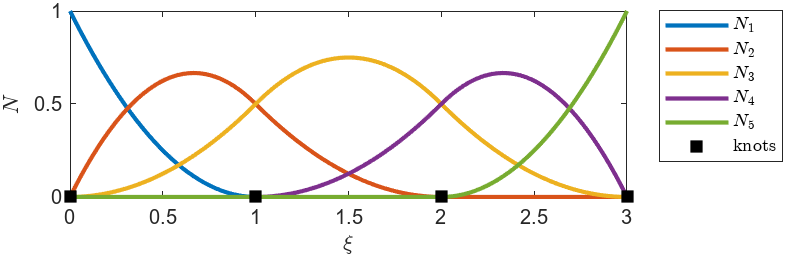
\includegraphics[width=0.8\linewidth]{Images/NURBS_1.jpg}
  \caption{B-Splines }
\end{subfigure}\\[1ex] % Add some vertical space between subfigures
\begin{subfigure}{0.8\textwidth}
  \centering
  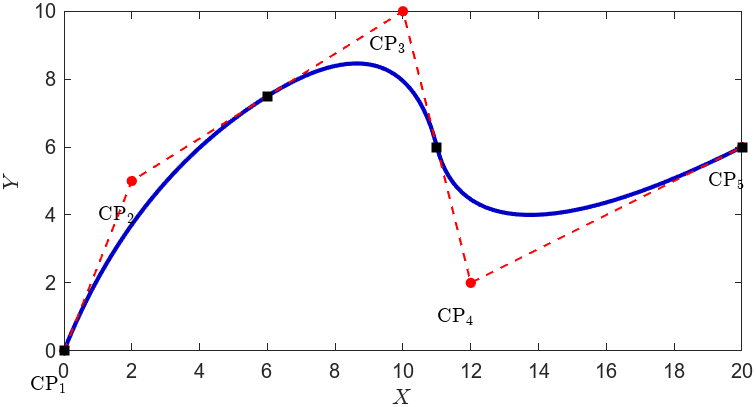
\includegraphics[width=0.8\linewidth]{Images/nCurve_1.png}
  \caption{B-Spline Curve}
\end{subfigure}
\caption{ $\xi=[0, 0, 0, 1, 2, 3, 3, 3]$ and $w=[1,1,1,1,1]$ }
\label{fig:curve1}
\end{figure}
\subsection{Continuity} \label{sec:continuity}
The only difference between the two figures lies the their knot vectors. It must be noted that the continuity at any parametric point is $C^{p-k}$, where $p$ is the polynomial degree and $k$ is the repetition of the knot value. In figure \ref{fig:curve2}, the knot 1 is repeated 2 times and the polynomial order is also 2. Hence the continuity reduces to $C^{2-2}=C^0$, and  the control point $CP_2$ is interpolated and a kink is seen in the curve.
\par 
The continuity between the knots of the knot vector is $C^{\infty}$.

\begin{figure}[H]
\centering
\begin{subfigure}{0.8\textwidth}
  \centering
  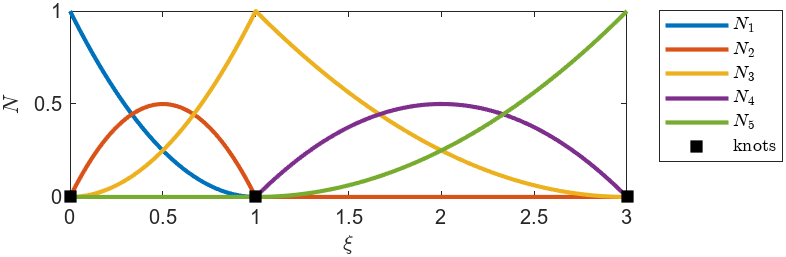
\includegraphics[width=0.8\linewidth]{Images/NURBS_2.jpg}
  \caption{B-Splines }
\end{subfigure}\\[1ex] % Add some vertical space between subfigures
\begin{subfigure}{0.8\textwidth}
  \centering
  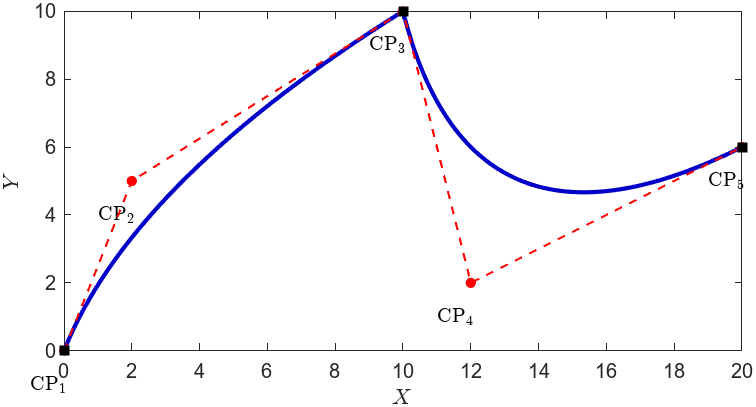
\includegraphics[width=0.8\linewidth]{Images/nCurve_2.png}
  \caption{B-Spline Curve}
\end{subfigure}
\caption{ $\xi=[0, 0, 0, 1, 1, 3, 3, 3]$ and $w=[1,1,1,1,1]$ }
\label{fig:curve2}
\end{figure}

\section{Basis Functions:~~NURBS}
\par
B-Splines cannot generate all conic section geometries like a circle (see figure \ref{fig:bspl_comp}). Then comes the need for NURBS which are a generalization of B-Splines. The name stands for Non-Uniform Rational B-Splines. Each basis function corresponding to a control point has a weight that defines the influence of that control point. The weights of all the B-Spline basis functions is 1.
The NURBS curve generation formula is given respectively as follows:
\begin{align}
C_N(\xi) &= \sum_{i=1}^{n} R_{i,p}(\xi)P_i\\
\text{where the NURBS basis function}~~ R_{i,p} &=  \frac{N_{i,p}(\xi)w_i}{\sum_{i=1}^{n} N_{i,p}(\xi)w_i}
\end{align}

\subsection{Effect of Weights}
As seen in figure \ref{fig:curve3}, the weight corresponding to $CP_3$ is decreased from 1 to 0.3. Its influence on the curve can be seen decreasing (compare to figure \ref{fig:curve1}). Weights can be greater than 1, which dominates the effect of the corresponding control point relative to a B-spline control point.
\begin{figure}[H]
\centering
\begin{subfigure}{0.4\textwidth}
  \centering
  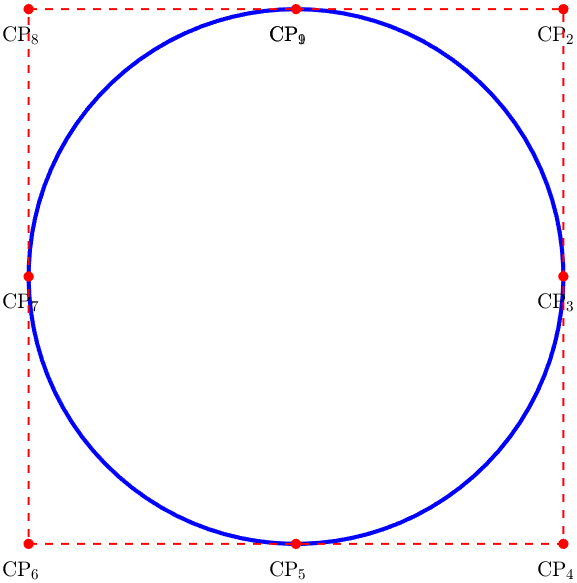
\includegraphics[width=\linewidth]{Images/cir1.png}
  \caption{Using NURBS}
  \label{fig:simple_cir}
\end{subfigure}\hfill
\begin{subfigure}{0.4\textwidth}
  \centering
  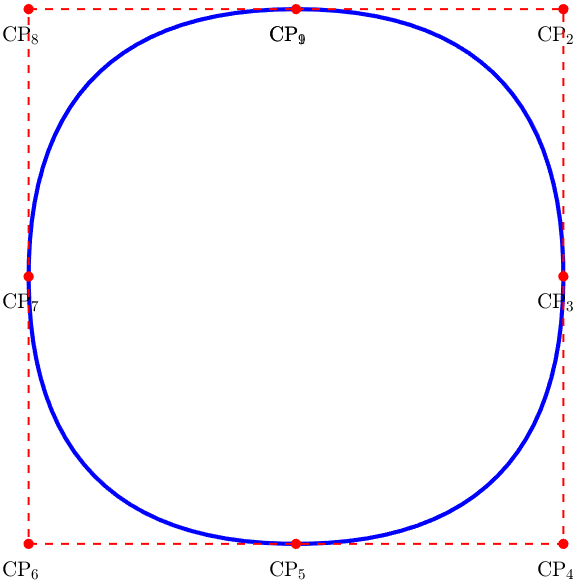
\includegraphics[width=\linewidth]{Images/cir2.png}
  \caption{Using B-Splines}
\end{subfigure}
\caption{Comparison of a circles generated using NURBS and B-Splines }
\label{fig:bspl_comp}
\end{figure}

\begin{figure}[H]
\centering
\begin{subfigure}{0.8\textwidth}
  \centering
  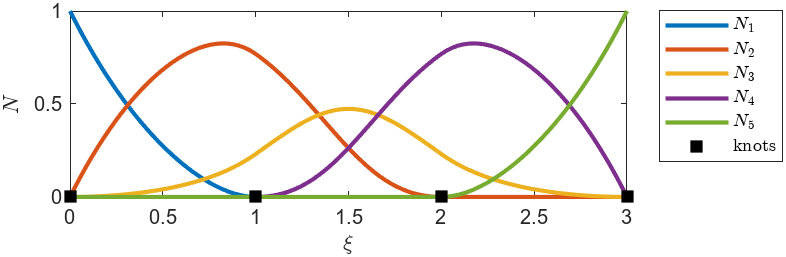
\includegraphics[width=0.8\linewidth]{Images/NURBS_3.jpg}
  \caption{NURBS Basis Functions }
\end{subfigure}\\[1ex] % Add some vertical space between subfigures
\begin{subfigure}{0.8\textwidth}
  \centering
  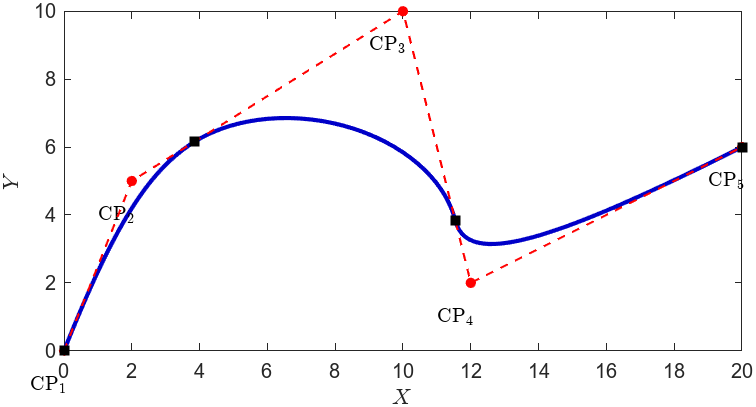
\includegraphics[width=0.8\linewidth]{Images/nCurve_3.png}
  \caption{NURBS Curve}
\end{subfigure}
\caption{ $\xi=[0, 0, 0, 1, 2, 3, 3, 3]$ and $w=[1,1,0.3,1,1]$ }
\label{fig:curve3}
\end{figure}

The extension of curves to surface(B-Spline or NURBS) is simple and straightforward. A surface has two parametric directions $[\xi,\eta]$ unlike curves which only has one. Hence a surface has two knot vectors and two polynomial degrees [p,q].

\begin{align}
S_N(\xi, \eta) &=\frac{\sum_{k=1}^{n} \sum_{l=1}^{m} N_{k,p}(\xi)M_{l,q}(\eta)w_{k,l} P_{i,j}}{\sum_{i=1}^{n} \sum_{j=1}^{m} N_{i,p}(\xi)M_{j,q}(\eta)w_{i,j} } 
\end{align}
A NURBS surface like the one shown in figure \ref{fig:nurb_surf} has diverse control point weights with values 1, $\frac{1}{\sqrt{2}}$ and also $\frac{1}{2}$. Thus surfaces like these cannot be generated as B-spline surfaces. 
\begin{figure}[H]
\centering
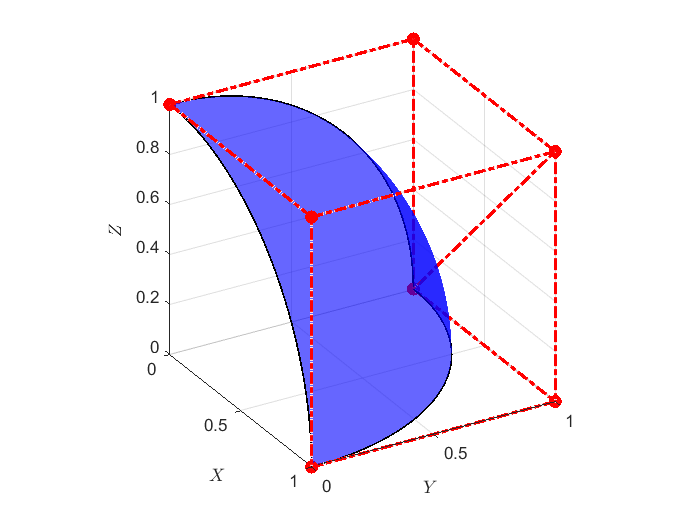
\includegraphics[width=0.8\linewidth]{Images/nurbs_surf.png}
\caption{$\frac{1}{8^{th}}$ of a shpere generated as a NURBS surface}
\label{fig:nurb_surf}
\end{figure}



\section{Isogeometric Analysis (IGA)}
 Apart from the inefficient meshing process, there are a few more limitations of FEA. For instance, the continuity between the mesh elements in traditional FEA is $C^0$. This poses a unique problem in analyzing certain physical problems like the Euler-Bernoulli beam or Kirchhoff-Love shell, which demand a higher continuity between elements. 
 \par
 Since we use the same basis functions of the CAD domain(i.e., NURBS), there is considerable freedom in choosing the continuity between the elements as long as the geometrical continuity is fulfilled.
 Finally comes the refinement. Although the h-refinement in IGA is not purely local because of the cross-product nature of NURBS surfaces, however the concept is fairy simple. And one good feature about IGA is that the same geometry can be represented by any increment of polynomial degree of basis functions or by any addition of elements in either direction. Table \ref{tab:1} shows the comparison between IGA and FEA.


\begin{table}[h!]
\begin{center}
\begin{tabular}{|c|c|}
    \hline
    \textcolor{blue}{Isogeometric Analysis} & \textcolor{blue}{Finite Element Analysis} \\ 
    \hline
    \text{No meshing required} & \text{Meshing required}  \\
    \hline
    \text{Uses NURBS basis functions} & \text{Uses Lagrange Polynomials} \\
    \hline
    \text{Any continuity between elements} & \text{Usually not higher than $C^0$ continuity} \\
    \hline
    \text{Refinement preserves original geometry} & \text{Refinement distorts geometry} \\
    \hline
    \text{Still mostly in research and development} & \text{Standard in industry} \\
    \hline
\end{tabular}
\caption{Comparison between IGA and FEA}
\label{tab:1}
\end{center}
\end{table}
 
\subsection{Concept of an element in IGA} \label{sec: iga_el}
Elements in conventional FEM refer to the actual mesh part created on the surface geometry.It can be triangular, quadrilateral etc. Since no mesh is created IGA on the geometry, the concept of element arises from the knot vectors. Knot spans in both the parametric directions form the domain of the elements for a surface and like wise each knot span of the knot vector corresponds to an element for a curve. Consider figure \ref{fig:curve1}, the knot vector of the curve is [0,0,0,1,2,3,3,3]. Thus the knot spans are [0,1], [1,2] and [2,3] and hence the curve has three elements as can be seen as curve sections between the black dots (knots).
\begin{figure}[H]
\centering
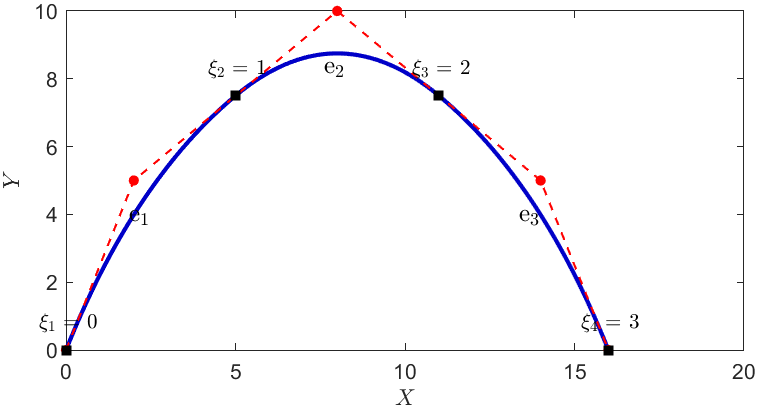
\includegraphics[width=0.8\linewidth]{Images/iga_element_curve.png}
\caption{Elemets of a curve based on the knot vector [0,0,0,1,2,3,3,3]}
\label{fig:crv_element}
\end{figure}
The same concept is extended for surfaces as well. The elements there correspond to the domains $\left( [\xi_i,\xi_{i+1}],[\eta_j,\eta_{j+1}]\right )$ 

\subsection{Refinement} \label{sec: iga_refinement}
The NURBS geometry is usually refined before performing IGA. The element concentration can be made dense (knot insertion)and/or the polynomial order can be increased (order elevation). These refinements preserve the geometry unlike FEM refinement which distorts the geometry.
\par It must be noted that throughout the refinement, the relation between polynomial degree, number of knots and the number of control points is not violated.
\begin{equation} \label{eq: mnp}
    m=n+p+1
\end{equation}
where $m$ is the number of knots in the knot vector, $n$ is the number of control points and $p$ is the polynomial degree.
We will see the effect of knot insertion and degree elevation indenpendently on the curve shown in figure \ref{fig:initial_refinement}
\begin{figure}[H]
\centering
\begin{subfigure}{.5\textwidth}
  \centering
  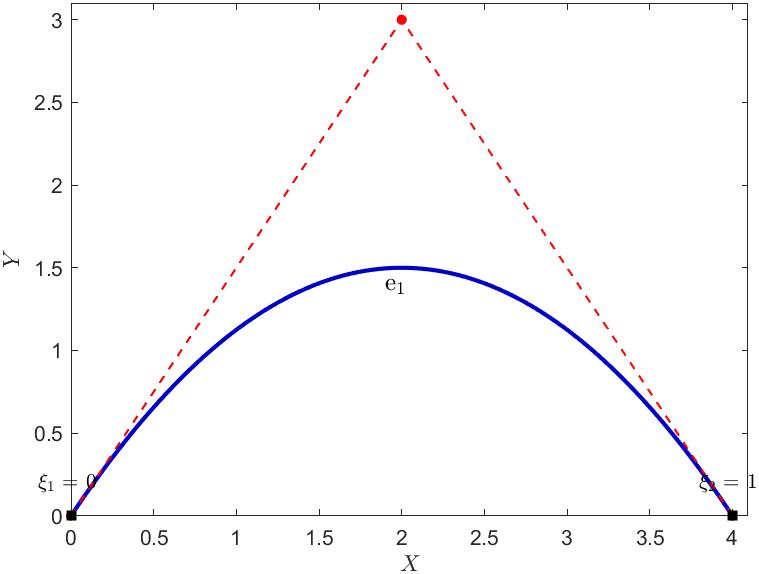
\includegraphics[width=1\linewidth]{Images/initial_curve.png}
  \caption{NURBS Curve}
  \label{fig:in_curve}
\end{subfigure}%
\begin{subfigure}{.6\textwidth}
  \centering
  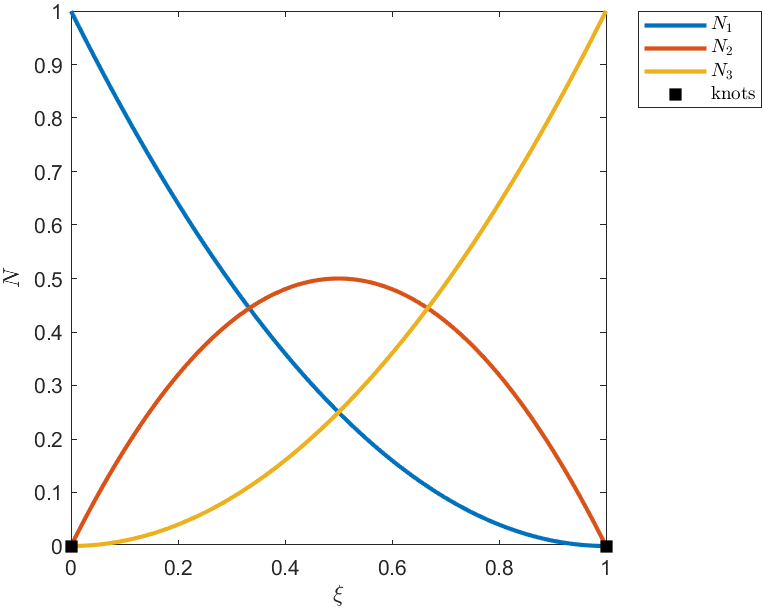
\includegraphics[width=0.6\linewidth]{Images/initial_basis.png}
  \caption{NURBS Basis}
  \label{fig:in_basis}
\end{subfigure}
\caption{Initial curve with knot vector [0,0,0,1,1,1]}
\label{fig:initial_refinement}
\end{figure}

\subsubsection{Knot insertion \cite{nurbs_refinement}} 
As already explained in section \ref{sec: iga_el}, each knot span corresponds to an element. So if we insert additional knots, it will naturally increase the number of elements in the geometry. And as per the equation \ref{eq: mnp}, additional control points have to be installed. The new control points can be found using $Boehm's algorithm$\cite{boehm}. Figure \ref{fig:href}, shows the new setting of the curve and the basis functions after performing h-refinement.
\begin{figure}[H]
\centering
\begin{subfigure}{.5\textwidth}
  \centering
  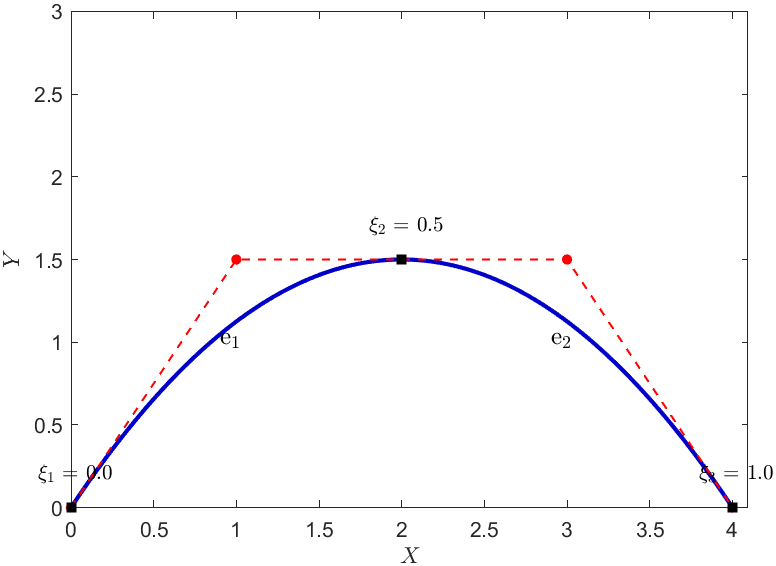
\includegraphics[width=1\linewidth]{Images/href_curve.png}
  \caption{NURBS Curve}
  \label{fig:href_curve}
\end{subfigure}%
\begin{subfigure}{.6\textwidth}
  \centering
  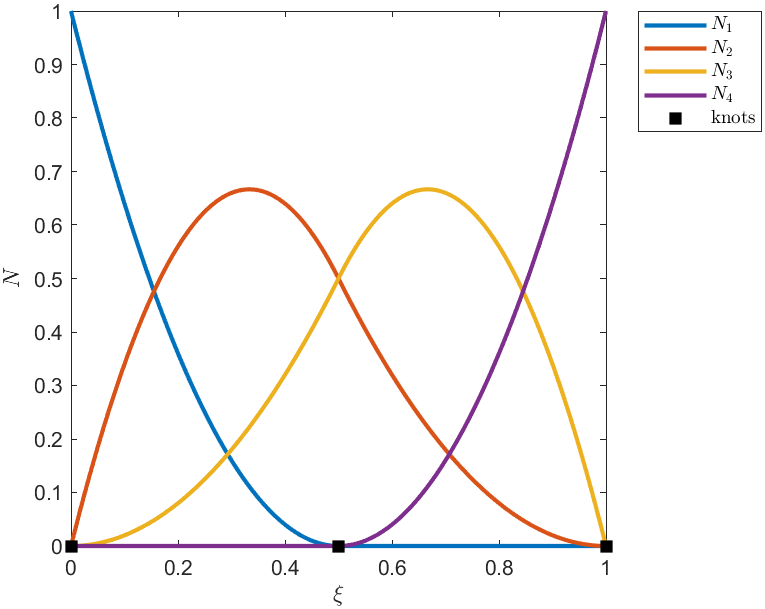
\includegraphics[width=0.6\linewidth]{Images/href_basis.png}
  \caption{NURBS Basis}
  \label{fig:href_basis}
\end{subfigure}
\caption{h-refined curve with knot vector [0,0,0,0.5,1,1,1]}
\label{fig:href}
\end{figure}
\subsubsection{Order elevation  \cite{nurbs_refinement}}
This refinement, as is clear from the name, increases the polynomial order of the basis functions with increasing the number of knots. In order to maintain the continuity at the knots $C^{p-k}$ ( see \ref{sec:continuity}), each existing knot is repeated and new control points computed in order to satisfy the equation \ref{eq: mnp}. F
Figure \ref{fig:pref}, shows the new setting of the curve and the basis functions after performing p-refinement on the original curve in figure \ref{fig:initial_refinement}.
\begin{figure}[H].
\centering
\begin{subfigure}{.5\textwidth}
  \centering
  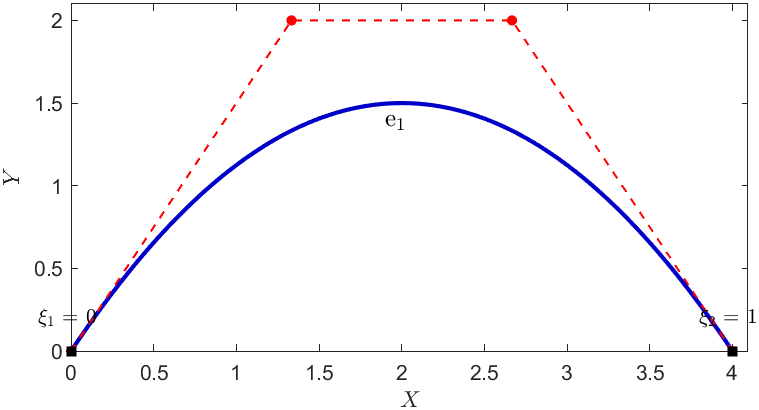
\includegraphics[width=1\linewidth]{Images/pref_curve.png}
  \caption{NURBS Curve}
  \label{fig:pref_curve}
\end{subfigure}%
\begin{subfigure}{.6\textwidth}
  \centering
  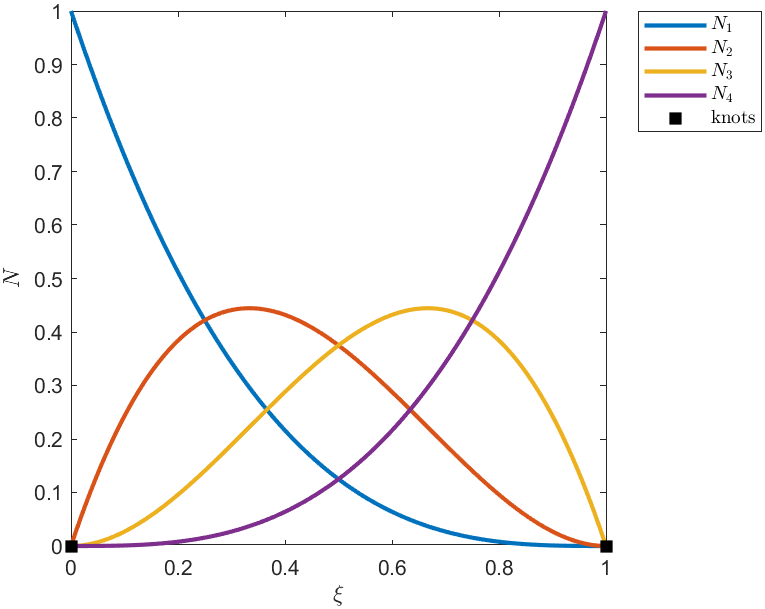
\includegraphics[width=0.6\linewidth]{Images/pref_basis.png}
  \caption{NURBS Basis}
  \label{fig:pref_basis}
\end{subfigure}
\caption{p-refined curve with knot vector [0,0,0,0,1,1,1]}
\label{fig:pref}
\end{figure}
\subsubsection{k refinement }
It must be noted that $h$ and $p$ refinements are not commutative. Usually $p$ refinement is performed first followed by $h$ refinement which yields better continuity across the space which is known as the $k$-refinement
\subsection{Weak Formulation}
Given a domain $\Omega$ with boundaries $\Gamma_D$ (Dirichlet)and $\Gamma_N$ (Neumann), the governing equilibrium is given by  \cite{iga_element}\cite{strong_eq}:
\begin{align}
\sigma_{i j, j}+f_{i} &=0 ~~\text{in}~~ \Omega\\
\mathbf{u}&=\mathbf{u}_{0} ~~\text{on}~~ \Gamma_{D}\\
\sigma_{i j} n_{j}&=\bar{t}_{i} ~~\text{on}~~ \Gamma_{N}
\end{align}
where $\sigma_{i j}$ is the Cauchy stress tensor, $n_j$ is the unit normal to the surface, $f_i$ the body force and $\bar{t_i}$ the traction force.
\par
As per the Hooke's law,
\begin{equation}
    \sigma_{i j}= C_{ijkl}\varepsilon_{kl}
\end{equation}
where $C_{ijkl}$ is the fourth order material constitutive tensor and $\varepsilon_{kl}$ is the strain tensor.
\par
If $S$ and $\partial S$ are the trial and virtual spaces such that $\mathbf{u} \in S$ and $\delta \mathbf{u} \in \partial S$, then the weak form is obtained as:
\begin{equation} \label{eq: weak}
   \Pi_{\mathrm{eq}}=\int_{\Omega} \varepsilon_{i j}(\mathbf{u}) C_{i j k l} \varepsilon_{k l}(\delta \mathbf{u}) \mathrm{d} \Omega-\int_{\Gamma_{t}} \bar{t}_{i} \delta u_{i} \mathrm{~d} \Gamma-\int_{\Omega} f_{i} \delta u_{i} \mathrm{~d} \Omega 
\end{equation}
The virtual displacement $\delta u_{i}$ represents the test function. It if often the case that the solution to the weak form cannot be found analytically and hence the problem is discretized to find the approximate solution.

\subsection{IGA Formulation}
As already mentioned, the distinct feature of IGA is the incorporation of NURBS basis functions. The geometry of the NURBS discretized element is simply given by:
\begin{equation}
    \mathbf{x}^{e}=\sum_{i=1}^{n_{c p}^{e}} R_{i} \mathbf{P}_{i}
\end{equation}
where $n_{c p}^{e}$ denotes the number of control points in an element. Using the isoparametric concept, same basis functions can be used for the solution field:
\begin{equation} \label{eq: iso_par}
    \mathbf{u}^{e}=\sum_{i=1}^{n_{c p}^{e}} R_{i} \mathbf{u}_{i}, \quad \delta \mathbf{u}^{e}=\sum_{i=1}^{n_{c p}^{e}} R_{i} \delta \mathbf{u}_{i}
\end{equation}
The stran displacement matrix for an isogeometric element is given by:
\begin{equation} \label{eq: b_mtx}
    \mathbf{B}=\left[\begin{array}{llllllllll}R_{1, x} & 0 & 0 & R_{2, x} & 0 & 0 & \cdots & R_{n_{c p}^{e}, x} & 0 & 0 \\ 0 & R_{1, y} & 0 & 0 & R_{2, y} & 0 & \cdots & 0 & R_{n_{c p}^{e}, y} & 0 \\ 0 & 0 & R_{1, z} & 0 & 0 & R_{2, z} & \cdots & 0 & 0 & R_{n_{c p}^{e}, z} \\ R_{1, y} & R_{1, x} & 0 & R_{2, y} & R_{2, x} & 0 & \cdots & R_{n_{c p}^{e}, y}^{e} & R_{n_{c p}^{e}, x} & 0 \\ 0 & R_{1, z} & R_{1, y} & 0 & R_{2, z} & R_{2, y} & \cdots & 0 & R_{n_{c p}^{e}, z} & R_{n_{c p}^{e}, y} \\ R_{1, z} & 0 & R_{1, x} & R_{2, z} & 0 & R_{2, x} & \cdots & R_{n_{c p}^{e}, z} & 0 & R_{n_{c p}^{e}, x}\end{array}\right]
\end{equation}

Substituting equations \ref{eq: b_mtx} and \ref{eq: iso_par} into \ref{eq: weak}, we get:
\begin{equation} \label{eq: iga_eqn}
\sum_{e=1}^{n e l}\left[\left(\int_{\Omega^{e}} \mathbf{B}^{\mathrm{T}} \mathbf{C B} \mathrm{d} \Omega\right) \mathbf{u}=\int_{\Gamma_{N}^{e}} \mathbf{R} \cdot \boldsymbol{t} \mathrm{d} \Gamma+\int_{\Omega^{e}} \mathbf{R} \cdot \boldsymbol{f} \mathrm{d} \Omega\right]
\end{equation}
where $\mathbf{R}$ is defined on the boundary as:
\begin{equation}
\mathbf{R}=\left[\begin{array}{ccccccc}R_{1}(\xi, \eta) & 0 & R_{2}(\xi, \eta) & 0 & \ldots & R_{n_{e p}^{e}}(\xi, \eta) & 0 \\ 0 & R_{1}(\xi, \eta) & 0 & R_{2}(\xi, \eta) & \ldots & 0 & R_{n_{e p}^{e}}(\xi, \eta)\end{array}\right]^{\mathrm{T}}   
\end{equation}
The standard form of the equation \ref{eq: iga_eqn} is given as:
\begin{equation}
    \sum_{e=1}^{n e l}\left[\mathbf{K}^{e} \mathbf{U}^{e}=\mathbf{F}^{e}\right]
\end{equation}
The assembly of element stiffness matrices follows the same procedure as for IGA.
\subsection{Integration of IGA elements} \label{sec: iga_ele_integration}
Integration as required in equation \ref{eq: iga_eqn} is computed element-wise using Gauss quadrature [p+1,q+1] points. Thus the stiffness matrix $\mathbf{K^e}$ of the element $\Omega^e$ is approximated as the sum of the product of the integrand computed at distrete Gauss points with corresponding weights and Jacobian mappings i,e.
\begin{align}
    \mathbf{K^e} = \int_{\Omega^{e}} \mathbf{B}^{\mathrm{T}} \mathbf{C B} \mathrm{d} \Omega
     = \sum_{1}^{n_g}\mathbf{B^T}(\xi_G,\eta_G)\mathbf{C}\mathbf{B}(\xi_G,\eta_G) \left |\mathbf{J_1}(\xi_G,\eta_G)\right| \left |\mathbf{J_2}(\xi_G,\eta_G)\right |w_{\xi_G}w_{\eta_G}
\end{align}
where the Jacobian $\mathbf{J_1}(\xi_G,\eta_G)$ is the mapping (see figure \ref{fig:1st_jacob}) from the physical space (x,y) to the parametric space $(\xi,\eta)$ evaluated at the Gauss point $(\xi_G,\eta_G)$ defined by:
\begin{equation}
    \mathbf{J_1}= \begin{bmatrix}
    \frac{\partial x}{\partial \xi} &  \frac{\partial y}{\partial \xi} \\
    \frac{\partial x}{\partial \eta} & \frac{\partial y}{\partial \eta}  \\
\end{bmatrix}
\end{equation}

\begin{figure}[H]
\centering
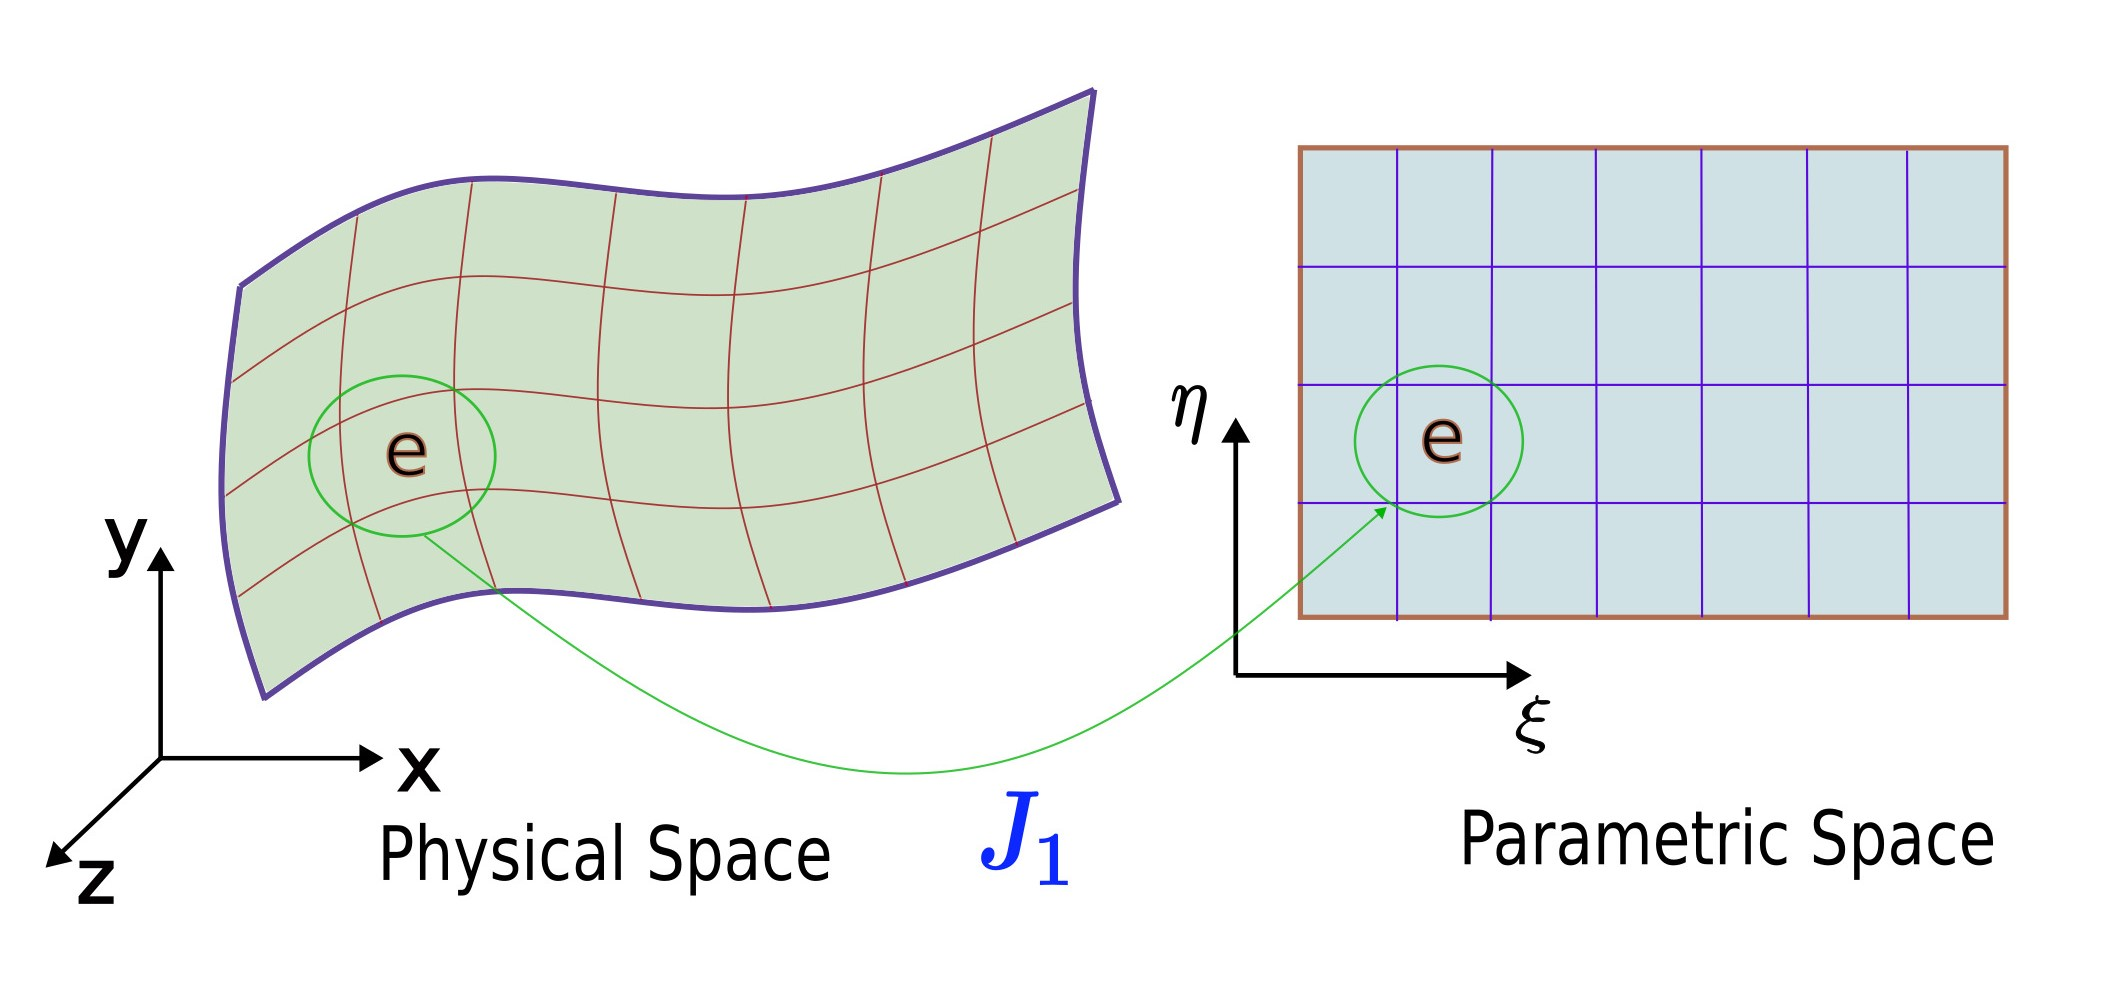
\includegraphics[width=0.8\linewidth]{Images/first_jacobiansvg.jpg}
\caption{Mapping elements from the physical space to the parametric space using the Jacobian $\mathbf{J_1}$ }
\label{fig:1st_jacob}
\end{figure}
And the Jacobian $\mathbf{J_2}(\xi_G,\eta_G)$ is the linear mapping (see figure \ref{fig:2nd_jacob}) from the parametric space (x,y) to the  Gaussian space $(\xi,\eta)$ evaluated at the Gauss point $(\xi_G,\eta_G)$ defined by:
\begin{equation}
    \mathbf{J_2}= \begin{bmatrix}
    \frac{\partial \xi}{\partial \xi_G} &  \frac{\partial \eta}{\partial \xi_G} \\
    \frac{\partial \xi}{\partial \eta_G} & \frac{\partial \eta}{\partial \eta_G}  \\
\end{bmatrix}
\end{equation}

\begin{figure}[H]
\centering
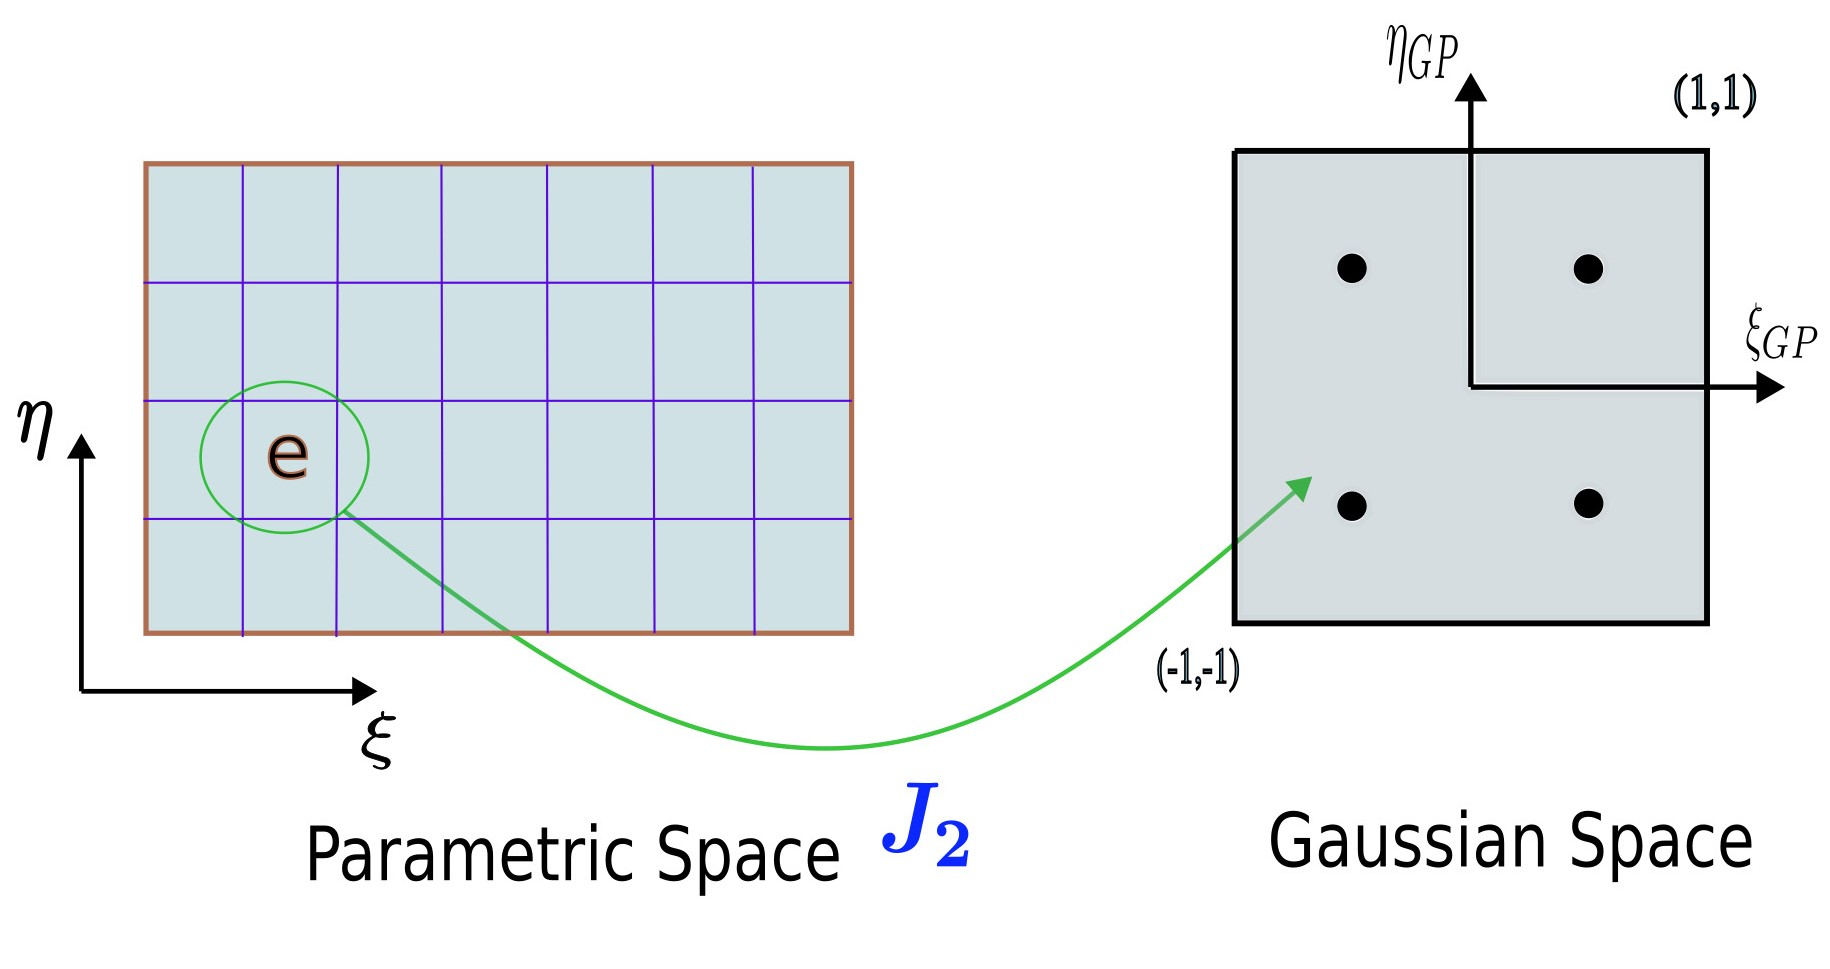
\includegraphics[width=0.8\linewidth]{Images/sec_jacobian.jpg}
\caption{Mapping an element from the parametric space to the  Gaussian space using the Jacobian $\mathbf{J_2}$ }
\label{fig:2nd_jacob}
\end{figure}
\subsection{CAD neutral formats and software used} \label{sec: neutral}
The CAD geometries were created in Rhino software and imported in the MATLAB App as vendor-neutral format IGES files. 


  

\chapter{Data Exchange with PythonOCC} \label{chap:PythonOCC}
PythonOCC is a 3D modeling Python package based on Open Cascade Technology through SWIG(Simple Wrapper Interface Generator) wrapper generator. To do Isogeometric Analysis in MATLAB for CAD geometries, the first task is to extract the necessary NURBS information from IGES files. We use PythonOCC\cite{pythonocc} in Python script to achieve this goal.

\setlength{\parskip}{12pt}
\section{Open Cascade Technology(OCCT)}
Open Cascade Technology(OCCT)\cite{occt} is an open-source 3D geometry library in C++ for CAD, CAM, CAE, CMM, and CAQ. OCCT is composed of C++ classes grouped into packages. The main features OCCT provides are Geometric modeling, surface and solid modeling, data exchange, and visualization. A subproject of PythonOCC, pythonocc-generator\cite{pythonocc-generator}, automatically generates the \href{https://www.swig.org/}{SWIG} interface files for the OpenCascade Python wrapper.

\setlength{\parskip}{12pt}
\section{PythonOCC}
PythonOCC is a free, open-source Python package developed and modified by Thomas Paviot. PythonOCC can be redistributed and modified under the terms of the GNU Lesser General Public License version 3 as published by the Free Software Foundation. PythonOCC provides full access from Python to most of OpenCascade C++ classes. The major features PythonOCC provides are like OpenCascade does, including 3D visualization from Python GUI, 3D modeling, data exchange, and various utility Python classes for Topology operation. 

\setlength{\parskip}{12pt}
\section{Installation for PythonOCC}
Here is an example\cite{pythonocc} of an installation with Anaconda Prompt:
\vspace{12pt}
\begin{lstlisting}{language=console, caption=Anaconda Prompt Commands}
conda install -c conda-forge pythonocc-core=7.7.2
\end{lstlisting}
For a specific version or a newer version, please adjust it accordingly.
If working in a new environment is preferable, an environment for PythonOCC can be created before installation like the following: 
\vspace{12pt}
\begin{lstlisting}{language=console, caption=Anaconda Prompt Commands}
conda create --name=pyoccenv python=3.9
source activate pyoccenv
\end{lstlisting}
Please adjust the name of the environment and the version of Python based on your specific case.
For more details about documentation, installation, and Demos of how PythonOCC works, please refer to the \href{https://github.com/tpaviot/pythonocc-core}{git repository}\cite{pythonocc}. Anaconda users can also refer to information on installation on the \href{https://anaconda.org/conda-forge/pythonocc-core}{Anaconda Website}.
 
\setlength{\parskip}{12pt}
\section{NURBS Information Extraction through PythonOCC}
We aim to extract information such as knot vectors, polynomial degrees, weights, and control points of NURBS curves and surfaces from IGES files. Thus, the main application we focus on for PythonOCC is the data exchange feature. The function
\vspace{0.5pt}
\begin{lstlisting}{language=Python}
read_iges_file(iges_file_path)
\end{lstlisting}
from OCC.Extend.DataExchange is already a PythonOCC function that contains all the necessary data exchange steps in OpenCascade to read an IGES file.
To convert a shape into NURBS geometry,
\vspace{12pt}
\begin{lstlisting}{language=Python}
nurbs_converter = BRepBuilderAPI_NurbsConvert(
                const TopoDS_Shape &S, 
                const Standard_Boolean Copy=Standard_False) 
converted_shape = nurbs_converter.Shape()
\end{lstlisting}
from OCC.Core.BRepBuilderAPI is implemented to get the converted shape. 
\vspace{12pt}
\begin{lstlisting}{language=Python}
explorer = TopologyExplorer(converted_shape)
\end{lstlisting}
from OCC.Extend.TopologyUtils is to explore how topological entities are connected from one to another. To access curves and surfaces, simply call the member function \texttt{edges()} and \texttt{faces()} like this:
\vspace{12pt}
\begin{lstlisting}{language=Python}
explorer.edges()
explorer.faces()
\end{lstlisting}
To get information of NURBS curves and surfaces, simply loop over all edges and faces from the explorer.

\vspace{12pt}
\begin{lstlisting}{language=Python}
curv = BRepAdaptor_Curve (const TopoDS_Edge &E) 
bcurve = curv.BSpline() 
\end{lstlisting}
from OCC.Core.BRepAdaptor creates a curve to access the geometry of edge <E> and make a copy of the BSpline curve. 
\vspace{12pt}
\begin{lstlisting}{language=Python}
surf = BRepAdaptor_Surface (const TopoDS_Face &F, 
     const Standard_Boolean R=Standard_True)
bsrf = surf.BSpline()
\end{lstlisting}
from OCC.Core.BRepAdaptor creates a surface to access the geometry of <F> and make a copy of the BSpline Surface. 

Finally, polynomial degrees, knot vectors, weights, and control points can be obtained by calling the member functions correspondingly.
\subsection{NURBS details of a curve}
The following is an example of extracting curve information during one of the explorer iterations: 
\vspace{12pt}
\begin{lstlisting}{language=Python}
curv = BRepAdaptor_Curve(edge)
bcurve = curv.BSpline()
curveDegree = bcurve.Degree()
knots = bcurve.Knots()
weights = bcurve.Weights()
poles = bcurve.Poles()
\end{lstlisting}
\texttt{curveDegree} is the polynomial order. \texttt{knots} is the knot vector. \texttt{weights} is the weights of all control points. \texttt{poles} is control points.
\subsection{NURBS details of a surface}
The following is an example of extracting surface information during one of the explorer iteration:
\vspace{12pt}
\begin{lstlisting}{language=Python}
surf = BRepAdaptor_Surface(face, True)
bsrf = surf.BSpline()
UCurveDegree = bsrf.UDegree()
VCurveDegree = bsrf.VDegree()
uknots = bsrf.UKnots()
vknots = bsrf.VKnots()
weights = bsrf.Weights()
poles = bsrf.Poles()
\end{lstlisting}
\texttt{UCurveDegree} and \texttt{VCurveDegree} are the polynomial order in \textbf{\textit{u}} and \textbf{\textit{v}}  direction. \texttt{uknots} and \texttt{vknots} are knot vectors in \textbf{\textit{u}} and \textbf{\textit{v}} direction. \texttt{weights} is the weights of all control points of the surface. \texttt{poles} is all control points of the surface.

\subsection{Trimming Curve-Surface parameter correlation}\label{sec: trim_corr}




To get more insight into how the OCCT classes and functions work, please refer to the \href{https://dev.opencascade.org/doc/occt-7.6.0/refman/html/files.html}{File List} of OpenCascade. The complete Python codes for extracting NURBS information of CAD geometries can be found in Appendix A. 

 

\chapter{MATLAB App - TUMIGA}\label{chap: App}


The App has been developed using \href{https://de.mathworks.com/products/matlab/app-designer.html}{MATLAB App Designer} which is an interactive object-oriented development environment for designing app layout and coding its behaviour. It provides a large set of interactive UI components which can be easily programmed using integrated version of MATLAB Editor. Additional user defined methods and properties can be created within proper classes.
\begin{figure}[H]
\centering
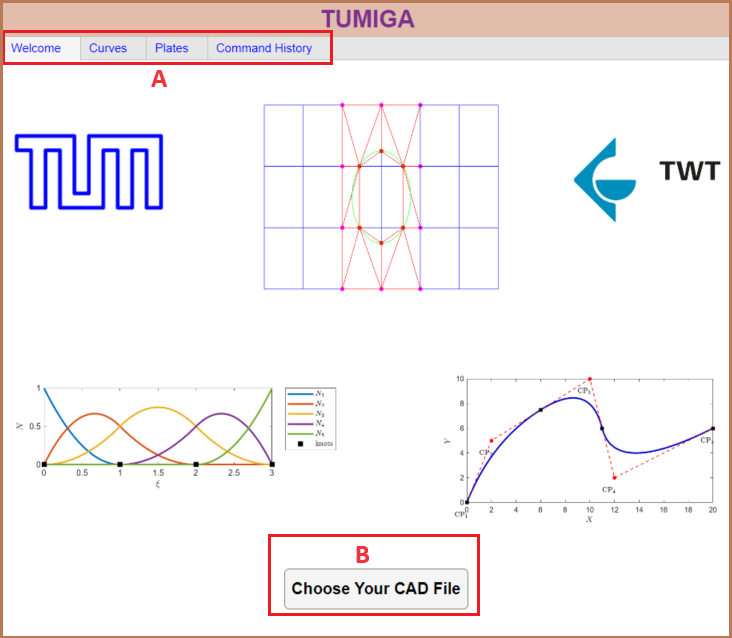
\includegraphics[width=0.6\textwidth]{Images/welcome.png}
\caption{Welcome page of TUMIGA}
\label{fig:welcome}
\end{figure}
\section{GUI}
\subsection{Welcome Page}
A highly interactive and visually appealing GUI was created keeping in mind that the knowledge of IGA possessed by the user may be limited. Hence anyone with basic knowledge of FEM, should also find it easy to use. When started, the welcome page appears (see A highlighted) and TUMIGA asks user to select a CAD geometry (see B highlighted) as shown in figure \ref{fig:welcome}. Once the user selects a geometry, TUMIGA takes the user to curves or plates page (see A highlighted in figure \ref{fig:welcome})  depending upon the dimension of the geometry. 

\subsection{Curves Page}
As mentioned in the abstract that for the sake of completion, analysis of Timoshenko beam is also possible. Three tabs are available on this page. One for design, one for analysis and one for post-processing. 
\begin{figure}[H]
\centering
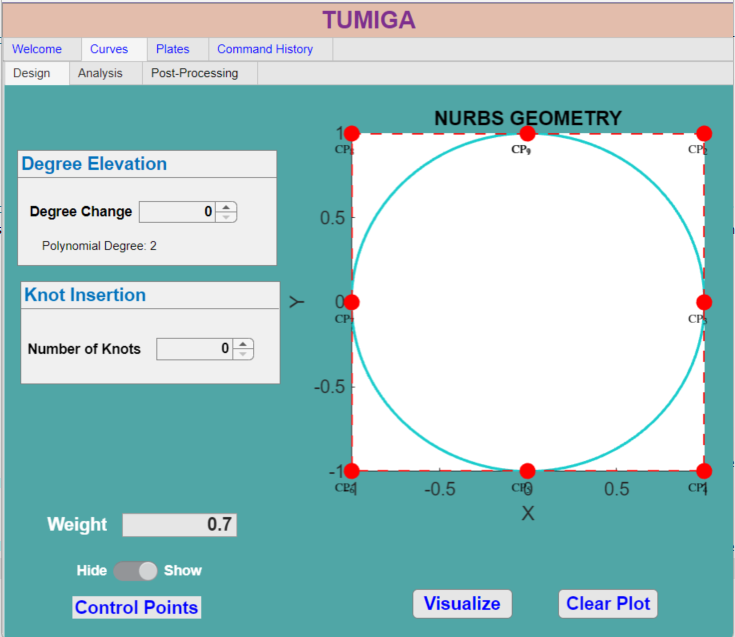
\includegraphics[width=0.6\textwidth]{Images/curves.png}
\caption{curves page-Design}
\label{fig:tumiga_curves_design}
\end{figure}
Degree elevation and knot refinement are offered as shown in figure \ref{fig:tumiga_curves_design}. Also control points can be seen, weights of odd points of circle can be modified.
\begin{figure}[H]
\centering
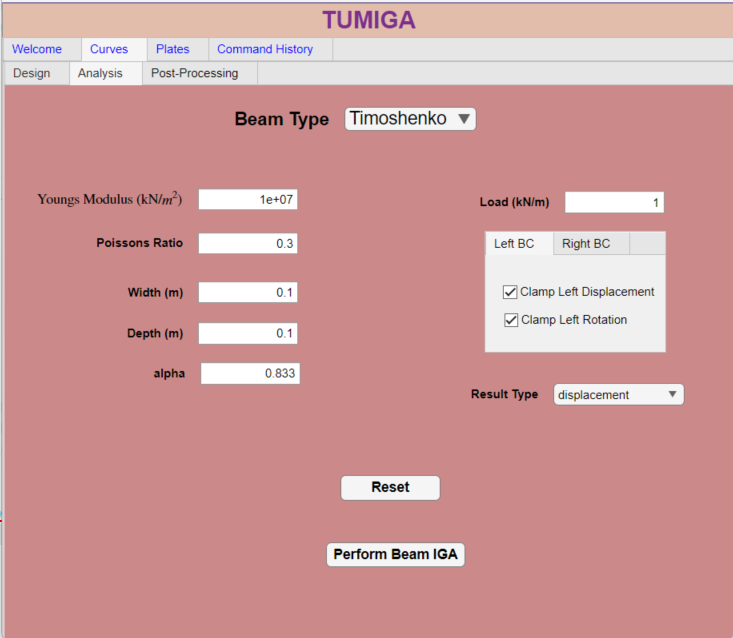
\includegraphics[width=0.6\textwidth]{Images/curves_analysis.png}
\caption{curves page-Analysis}
\label{fig:curves_analysis}
\end{figure}
In the analysis tab, material properties, loads (udl) and boundary conditions can be set (displacements and rotations on either of the two edges can be restricted) as shown figure \ref{fig:curves_analysis}. 
\begin{figure}[H]
\centering
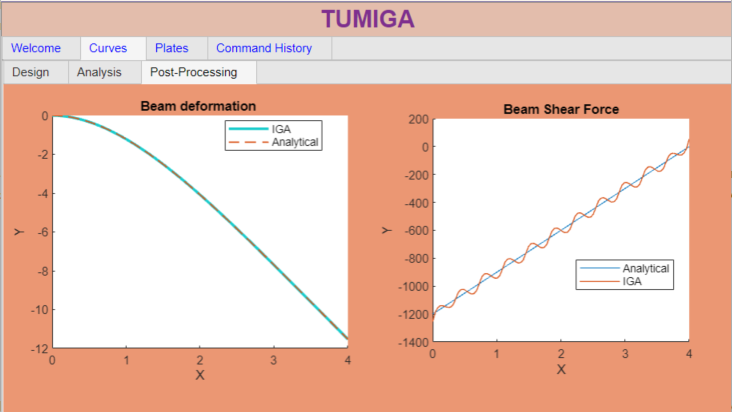
\includegraphics[width=0.6\textwidth]{Images/curves_postProcess.png}
\caption{curves page-Post-processing}
\label{fig:curves_process}
\end{figure}
Finally in the Post-Processing tab, results such as displacement and shear force can be viewed as shown figure \ref{fig:curves_process}. 

\subsection{Plates Page}
Comprehensive features are offered for plates as that forms the core of this thesis. Degree Elevation and Knot Refinement is offered in both parametric directions of all the patches of a multi-patch plate or shell. Surface plot properties are also provided including visibility of control polygons, elements and patch labels as shown in figure \ref{fig:plate_design}. 
\begin{figure}[H]
\centering
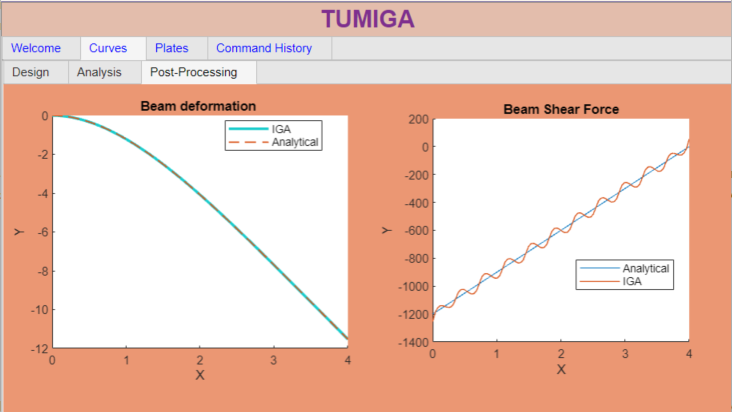
\includegraphics[width=0.6\textwidth]{Images/curves_postProcess.png}
\caption{Plates page-Post-Design}
\label{fig:plate_design}
\end{figure}

Advanced features are provided in the analysis tab, from material properties to setting Dirichlet boundary conditions and edge load directly on the edges (or trimming curves) of any patch of the geometry. Surface load for patches is also provided. Moreover, forces and boundary can be immediately visualized on UIAxes plot. Figure \ref{fig:plate_analysis} shows the analysis tab. As the button "\textbf{Set DBC on geometry}" is pushed, another user interface pops up (see figure \ref{fig:plate_pythonocc_popup} ) which was set up using PythonOCC. The "\textbf{File} and "\textbf{Selection}" buttons offer user to select faces (surfaces), edges, vertices from the geometry. Once done properly, the indicator turns green (see figure \ref{fig:plate_analysis}). "\textbf{Couple Patches} button automatically couples any number of patches using penalty method. 
\begin{figure}[H]
\centering
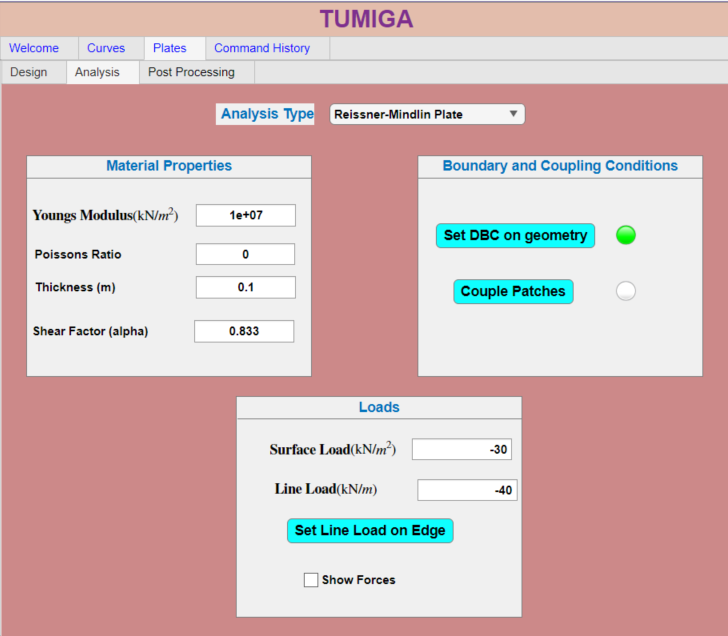
\includegraphics[width=0.6\textwidth]{Images/plate_analysis.png}
\caption{Plates page-Post-Analysis}
\label{fig:plate_analysis}
\end{figure}

\begin{figure}[H]
\centering
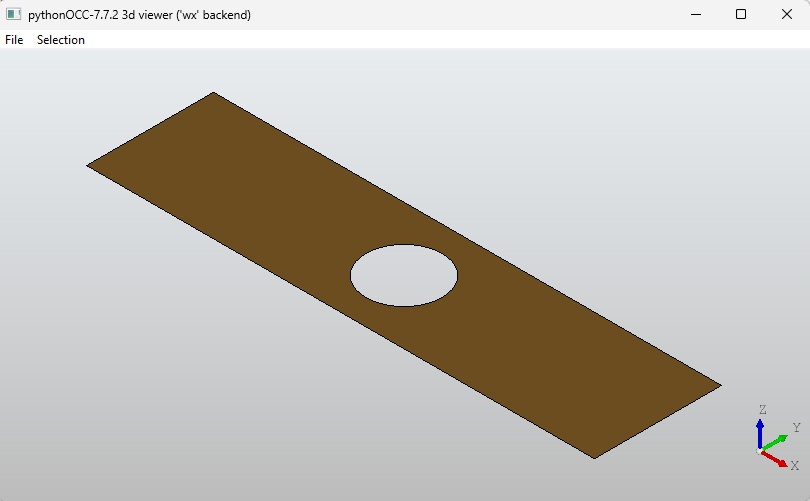
\includegraphics[width=0.7\textwidth]{Images/plate_pythonocc_popup.png}
\caption{User interface for setting DBCs and edge loads}
\label{fig:plate_pythonocc_popup}
\end{figure}
Like for the curves, a separate Post-Processing tab  for visualizing deflections and shear forces is provided.

\subsection{Command History}
This tab is provided if the user wants to see the history of his/her commands in the App. 

\section{Code View of TUMIGA}
A small discussion on the coding part would come very handy for interesting users. Each UI component that is visible on the user interface of the App, is programmed using the so called "\textbf{Callbacks}". What it means is that, how does a user wants it to behave and that is logically programmed. Each callback can be related to any other class or method or even another callback. Any number of user defined methods and properties can be defined in the classes. The first argument of any method when defined has to be "app" e.g, method\_a(app, arg\_1,arg\_2,...). Any property let us say propery\_x that is being called has to be written as "app.property\_x".
\section{Data Exchange with PythonOCC}
\subsection{Data as a Python Dictionary }

All the NURBS data in TUMIGA is obtained from PythonOCC library (see chapter \ref{chap:PythonOCC}). In python, these details are stored as dictionaries as shown below:
% Define custom colors
\definecolor{vscode-purple}{rgb}{0.502, 0, 0.502}
\definecolor{vscode-green}{rgb}{0, 0.502, 0}
\definecolor{vscode-blue}{rgb}{0, 0, 0.502}
\definecolor{vscode-yellow}{rgb}{0.502, 0.502, 0}
\definecolor{backcolour}{rgb}{0.95,0.95,0.92}% Light gray background

% Define custom Python style
\lstdefinestyle{python}{
    language=Python,
    backgroundcolor=\color{backcolour},
    commentstyle=\color{vscode-green},
    keywordstyle=\color{vscode-blue},
    numberstyle=\tiny\color{vscode-yellow},
    stringstyle=\color{vscode-purple},
    basicstyle=\ttfamily\small,
    breakatwhitespace=false,
    breaklines=true,
    captionpos=b,
    keepspaces=true,
    showspaces=false,
    showstringspaces=false,
    showtabs=false,
    tabsize=4,
    extendedchars=true,
    inputencoding=utf8,
    frame=tb,
    framerule=1pt,
    numbersep=5pt,
    numbers=left,
    stepnumber=1,  % Display every line number
    firstnumber=1   % Specify the starting line number
}

\lstset{style=python}
\begin{adjustwidth}{-0.5cm}{-0.5cm}
\begin{lstlisting}{language=Python}
from OCC.Core.BRepBuilderAPI import BRepBuilderAPI_NurbsConvert
from scipy.io import savemat
#..Importing classes
#...
#...

output_file = 'output.mat' # initiating a .mat file that is sent to TUMIGA

# Rest of the code
#...
#...

# Creating the dictionay...
    if isInner:
            
        my_dict = {'isTrim':1, 'uDeg': UCurveDegree,'vDeg': VCurveDegree,'uknotVector':UknotArr,
            'vknotVector':VknotArr,'weights':weightArray,'controlPoints':conPointMtx.T,
            'outer_wire':outer_wire_dict,'inner_wires':inner_wire_dict}
        
    else:
        my_dict = {'isTrim':0, 'uDeg': UCurveDegree,'vDeg': VCurveDegree,'uknotVector':UknotArr,
            'vknotVector':VknotArr,'weights':weightArray,'controlPoints':conPointMtx.T,'outer_wire':outer_wire_dict}
        
    fc_idx += 1
    dict_list.append(my_dict)  
    
data_to_save = {'dict_list': dict_list, 'dimension': geo_dim}
savemat(output_file, data_to_save)

\end{lstlisting}
\end{adjustwidth}

\subsection{Data as a .mat file }

The dictionary "data\_to\_save" has two entries, first "dict\_list" which contains the list of dictionaries of each patch of the geometry comprehensively including outer and inner trimming loops and the second entry "dimension" contains the dimension of the geometry (1 for curves and 2 for plates and shells). This dictionary is saved in a "output.mat" file. The code below shows the function in TUMIGA that reads this file and accesses/stores the NURBS details.
\definecolor{matlab-comment}{RGB}{34,139,34} % Dark green
\definecolor{matlab-keyword}{RGB}{0,0,255}   % Blue
\definecolor{matlab-string}{RGB}{160,32,240} % Purple
\definecolor{matlab-background}{RGB}{245,245,245} % Whitish background

% Define custom MATLAB style
\lstdefinestyle{matlab}{
    language=Matlab,
    backgroundcolor=\color{matlab-background},
    commentstyle=\color{matlab-comment},
    keywordstyle=\color{matlab-keyword},
    numberstyle=\tiny\color{vscode-yellow},
    stringstyle=\color{matlab-string},
    basicstyle=\ttfamily\small,
    breakatwhitespace=false,
    breaklines=true,
    captionpos=b,
    keepspaces=true,
    showspaces=false,
    showstringspaces=false,
    showtabs=false,
    tabsize=4,
    extendedchars=true,
    inputencoding=utf8,
    frame=tb,
    framerule=1pt,
    numbersep=5pt,
    numbers=left,
    stepnumber=1,  % Display every line number
    firstnumber=1   % Specify the starting line number
}

\lstset{style=matlab}

\begin{adjustwidth}{-0.5cm}{-0.5cm}
\begin{lstlisting}{language=Python}
function CallPythonScript(app, filePath)
    %Specify the full path to Anaconda Python executable
    anacondaPythonExecutable = 'C:\Users\......\python.exe';
    pythonScript = 'C:\Users\.......\outer_inner_wires.py';
    outputFile = 'output.mat';
    %Check if Anaconda Python executable exists
    if exist(anacondaPythonExecutable, 'file') == 2
        %Build the command
        command = sprintf('%s "%s" "%s"', anacondaPythonExecutable, pythonScript, filePath);
        %Call Python script
        [status, ~] = system(command, '-echo');
        if status == 0
            data = load(outputFile);
            dict_=data.dict_list;
            app.dict_list=dict_;        % to store original geometry
            app.change_dict_list=dict_;     % to store changed geometry
            app.deg_dict_list=dict_;        % to store degree refined geometry
            num_patches=numel(dict_);
            app.dim=data.dimension;
            app.num_patch=num_patches;
            app.updateLabelDropDown();  % Dropdown should have as many labels as the number of patches
            if app.dim==2
                num_points_poly=size(app.change_dict_list{1}.outer_wire.outer_Trim_Polygon,1);
                app.outer_poly=zeros(num_points_poly,2,num_patches);
                for i=1:num_patches
                    app.outer_poly(:,:,i)=app.change_dict_list{i}.outer_wire.outer_Trim_Polygon;
                end
            end
        else
            disp('File Not Found');
        end
    else
        disp('Anaconda Python executable not found. Please check the path.');
    end
    outCom=evalc('disp("Python called Successfully")');
    app.updateCommandHistory(outCom);
    app.begin=0;
    app.updatePlot;
end

\end{lstlisting}
\end{adjustwidth}



\chapter{Plate Analysis} \label{chap: Plate}
A plate is a structural element with two of its dimensions considerably larger than the third one (thickness). One of the  distinguishing feature of a plate is that in its undeformed shape it has no curvature i.e., it is plane. Based on the slenderness (thickness to length ratio) of the plate, different theories govern its behaviour. If the slenderness ratio is between 0.1 to 0.2, the plate is moderately thick and the Reisner-Mindlin theory governs its behaviour taking into considerations the transverse shear deformations and allowing the cross-sections to change the angle relative to the mid-plane.
\par For thin plates with slenderness ratio between 0.02 to 0.2, Kirchhoff-Love theory is applied with the assumption that shear deformations are negligible. Very thin plates with slenderness ratio less than 0.02 depict geometrically non-linear behaviour and are governed by von Karman theory which takes into consideration the membrane action. However, the finite element code in standard software for the analysis of shells is typically based on Reissner-Mindlin theory because of only $C^0$ continuity requirement which is easily fulfilled with lower order basis functions. This also introduces some unwanted effects like locking phenomenon giving rise to spurious shear stresses. 
During analysis, the plate is represented by the mid-surface with a bi-axial state of stresses and strains.
\section{Element Formulation}
The local displacements and strains on the plate's surface can be expressed as:\cite{plate1}
\begin{gather}
\boldsymbol{w(x,y,z)} = w_0(x,y)\\
\boldsymbol{u(x,y,z)}=z\varphi_x(x,y)\\
\boldsymbol{v(x,y,z)}=z\varphi_y(x,y);\\
\boldsymbol{\varepsilon_x}= \frac{\partial \boldsymbol{u}}{\partial x}=z.\frac{\partial \varphi_x}{\partial x}\\
\boldsymbol{\varepsilon_y}= \frac{\partial \boldsymbol{v}}{\partial y}=z.\frac{\partial \varphi_y}{\partial y}\\
\boldsymbol{\varepsilon_z}= \frac{\partial \boldsymbol{w}}{\partial z}=0\\
\boldsymbol{\gamma_{xz}} = \frac{\partial u}{\partial z} + \frac{\partial w}{\partial x}\\
\boldsymbol{\gamma_{yz}} = \frac{\partial v}{\partial z} + \frac{\partial w}{\partial y}\\
\boldsymbol{\gamma_{xy}} = \frac{\partial u}{\partial y} + \frac{\partial v}{\partial x}
\end{gather}

$\boldsymbol{w}$, $\boldsymbol{u}$ and $\boldsymbol{v}$ denote respectively the displacements in \textbf{\textit{z}}, \textbf{\textit{x}} and \textbf{\textit{y}} directions. $\boldsymbol{\varepsilon_x}$, $\varepsilon_y$  and $\varepsilon_z$ denote respectively the normal strains while $\gamma_{xz}$, $\gamma_{yz}$ and $\gamma_{xy}$ denote respectively the shear strains.
The combined normal and shear strains in a vector can be written as:
\begin{equation}
    \boldsymbol{\varepsilon}=z\boldsymbol{\kappa}
\end{equation}
where $\boldsymbol{\kappa}$ is the curvature vector:
\vspace{-50pt}
\begin{center}
\begin{equation}
\boldsymbol{\kappa} = 
\left\{
\begin{array}{c}
\frac{\partial \varphi_x}{\partial x} \\
\frac{\partial \varphi_y}{\partial y} \\
\begin{aligned}
\frac{\partial \varphi_x}{\partial y}+ \frac{\partial \varphi_y}{\partial x}
\end{aligned}
\end{array}
\right\}
\end{equation}
\end{center}

The kinematic equation is given as: 
\begin{equation}
\boldsymbol{L}\boldsymbol{\varphi}=\boldsymbol{\kappa}~~where~ \boldsymbol{L} =\begin{bmatrix}
    \frac{\partial}{\partial x} &  0 \\
    0 & \frac{\partial}{\partial y}  \\
    \frac{\partial}{\partial y} & \frac{\partial}{\partial x}
\end{bmatrix}
\end{equation}
The constitutive and equilibrium equations are given as:
\begin{align}
    \boldsymbol{m}&=\boldsymbol{D_b}\boldsymbol{\kappa}~~~~~~\boldsymbol{q}=\boldsymbol{D_s}\boldsymbol{\gamma}\\
    \boldsymbol{L^T}&\boldsymbol{m}-\boldsymbol{q}= 0~~~~ \boldsymbol{\nabla^T}\boldsymbol{q}+p=0
\end{align}
$\boldsymbol{m}$, $\boldsymbol{q}$ refer to vectors of moments and shear stresses. $\boldsymbol{D_b}$, $\boldsymbol{D_s}$ refers to material matrices for bending and shear respectively, $\boldsymbol{L}$ refers to the differential matrix and $p$ refers to the uniform surface forces.


\chapter{Shell Analysis} \label{chap: Shell}

\section{Element Formulation}


\chapter{Trimmed CAD geometries and IGA} \label{chap: Trimmed IGA}
Trimming is an essential procedure in the design of CAD geometries. Since a NURBS patch is essentially a quadrangular topological surface, to design real-life mechanical parts, one has to define the geometry within the patch by the curves which are known as trimming curves. It is achieved by making only the useful part of the geometry visible and hiding the rest. 
\section{Trimmed NURBS Curves}
\begin{figure}[H]
\centering
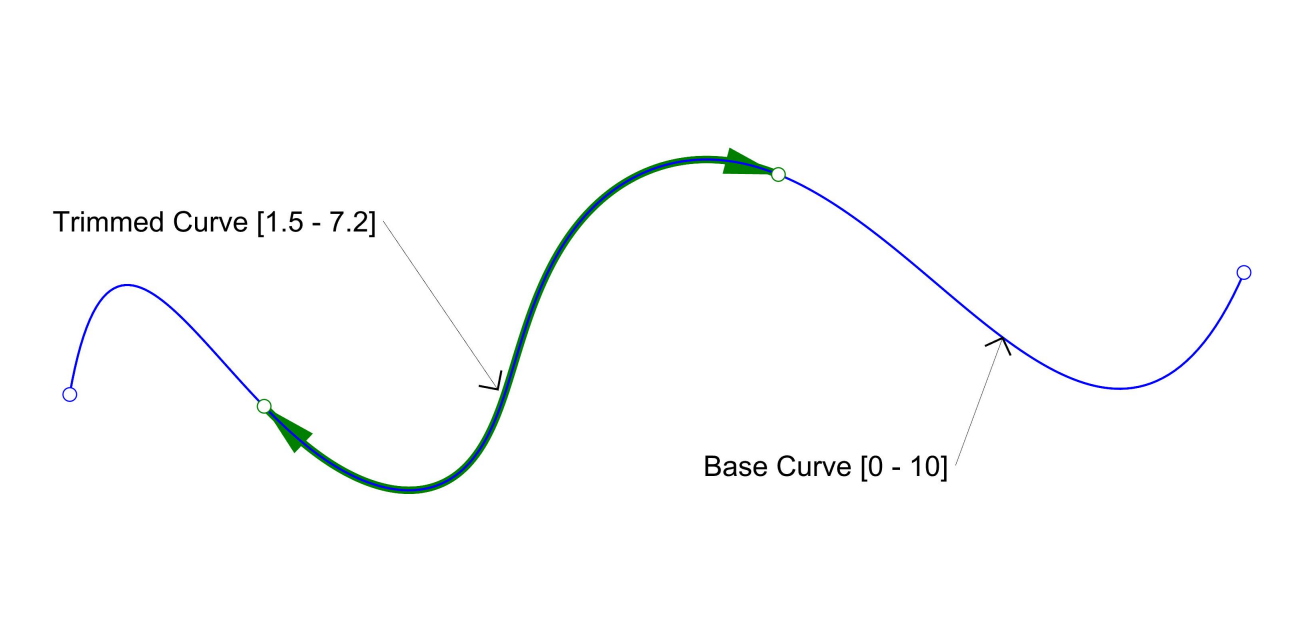
\includegraphics[width=0.8\textwidth]{Images/trimCurveDemo.png}
\caption{Trimmed Curve}
\label{fig:trCurv}
\end{figure}
A trimmed NURBS curve $\mathbf{C_{visible}}$ with a parametric domain $\mathcal{D}$ is the visible part of the original NURBS curve $\mathbf{C}$ with the parametric domain $\mathcal{H}$ such that:
\begin{align}
\mathcal{D} &= \{\xi \in \mathcal{H} \mid \xi_{\text{start}} \leq \xi \leq \xi_{\text{end}}\} \\
\mathbf{C_{vis}} &= \mathbf{C(\xi)} \mid \xi \in \mathcal{D}
\end{align}

Figure \ref{fig:trCurv} shows a trimmed curve defined within the domain [1.5 7.2] of the original domain [0 10].


\section{Trimmed NURBS Surfaces}
Like the trimming curves, trimmed surfaces are also created from the original patches by the omission of the surface within a certain domain. It does not anyhow change the NURBS details of the underlying complete surface. Figure \ref{fig:tSurf} shows a rectangular surface with a trimmed circular hole. As is clear, the control points still exist within the trimmed region.
Thus the domain of the trimmed surface is given by:
\begin{equation} 
\mathcal{D} = \{ (\xi, \eta) \in \mathcal{H} \mid \partial \mathcal{D} = \bigcup_{k=1}^{M} \mathbf{C}_k^{\sim} \}
\end{equation}
where $ \partial \mathcal{D}$ describes the closed boundary of the trimmed domain $\mathcal{D}$.
\newline
While dealing with NURBS surfaces, it is convenient to have the trimming curves too as NURBS curves such that there is a clear mapping between the parameters of the surface ($\xi, \eta$) and the parameter of the curve 
\begin{equation}
\mathbf{\tilde{C}}_{k}(\tilde{\xi}) = \begin{bmatrix} \xi_k(\tilde{\xi}) \\ \eta_k(\tilde{\xi}) \end{bmatrix} = \sum_{i=1}^{n_k} R_{i,l}^{(k)}(\tilde{\xi}) \mathbf{\tilde{P}}_{i}^{(k)}, \quad k = 1, 2, \ldots, M. \label{eq: trim_curve}
\end{equation}
where $l$ is the polynomial degree, $\tilde{\xi}$ is the curve parameter, $\xi_k$ and $\eta_k$ are
parameters of the surface representing the trimming curve $\mathbf{\tilde{C}}_{k}$ and $\mathbf{\tilde{P}}_{i}^{(k)}$ are
the control points of the trimming curve in the parameter space of the
surface. The curves $\mathbf{\tilde{C}}_{k}$ are joined properly to form outer and inner loops. The outer loops (with material inside) are oriented counter-clockwise, whereas the inner loops (with no material inside) are oriented clockwise (see figure \ref{fig:trim_el_type}).

\section{Methods of trimmed IGA}\label{subsection: methods_trim_iga}
As has been said already, a trimmed surface consists of a trimming curve (usually a NURBS curve) which has its own independent parametrization. The first step for the analysis then is to develop a correlation as expressed by \eqref{eq: trim_curve} between the parameter of the curve $\tilde{\xi}$ and the parameters of the surface $(\xi, \eta)$. This correlation is not available directly from a CAD software (see section \ref{sec: neutral}) and was achieved by PythonOCC (see section \ref{sec: trim_corr}). After required refinement of the surface, the intersection of the curve with the surface elements(see section \ref{sec: iga_el}) is sought. Depending on the intersection (i.e, the location of element vertices relative to the trimming curve) of the curve with the surface, an element may be inactive or active. Hence classifying an element by finding intersection points forms the basis of the analysis.
\begin{figure}[H]
\centering
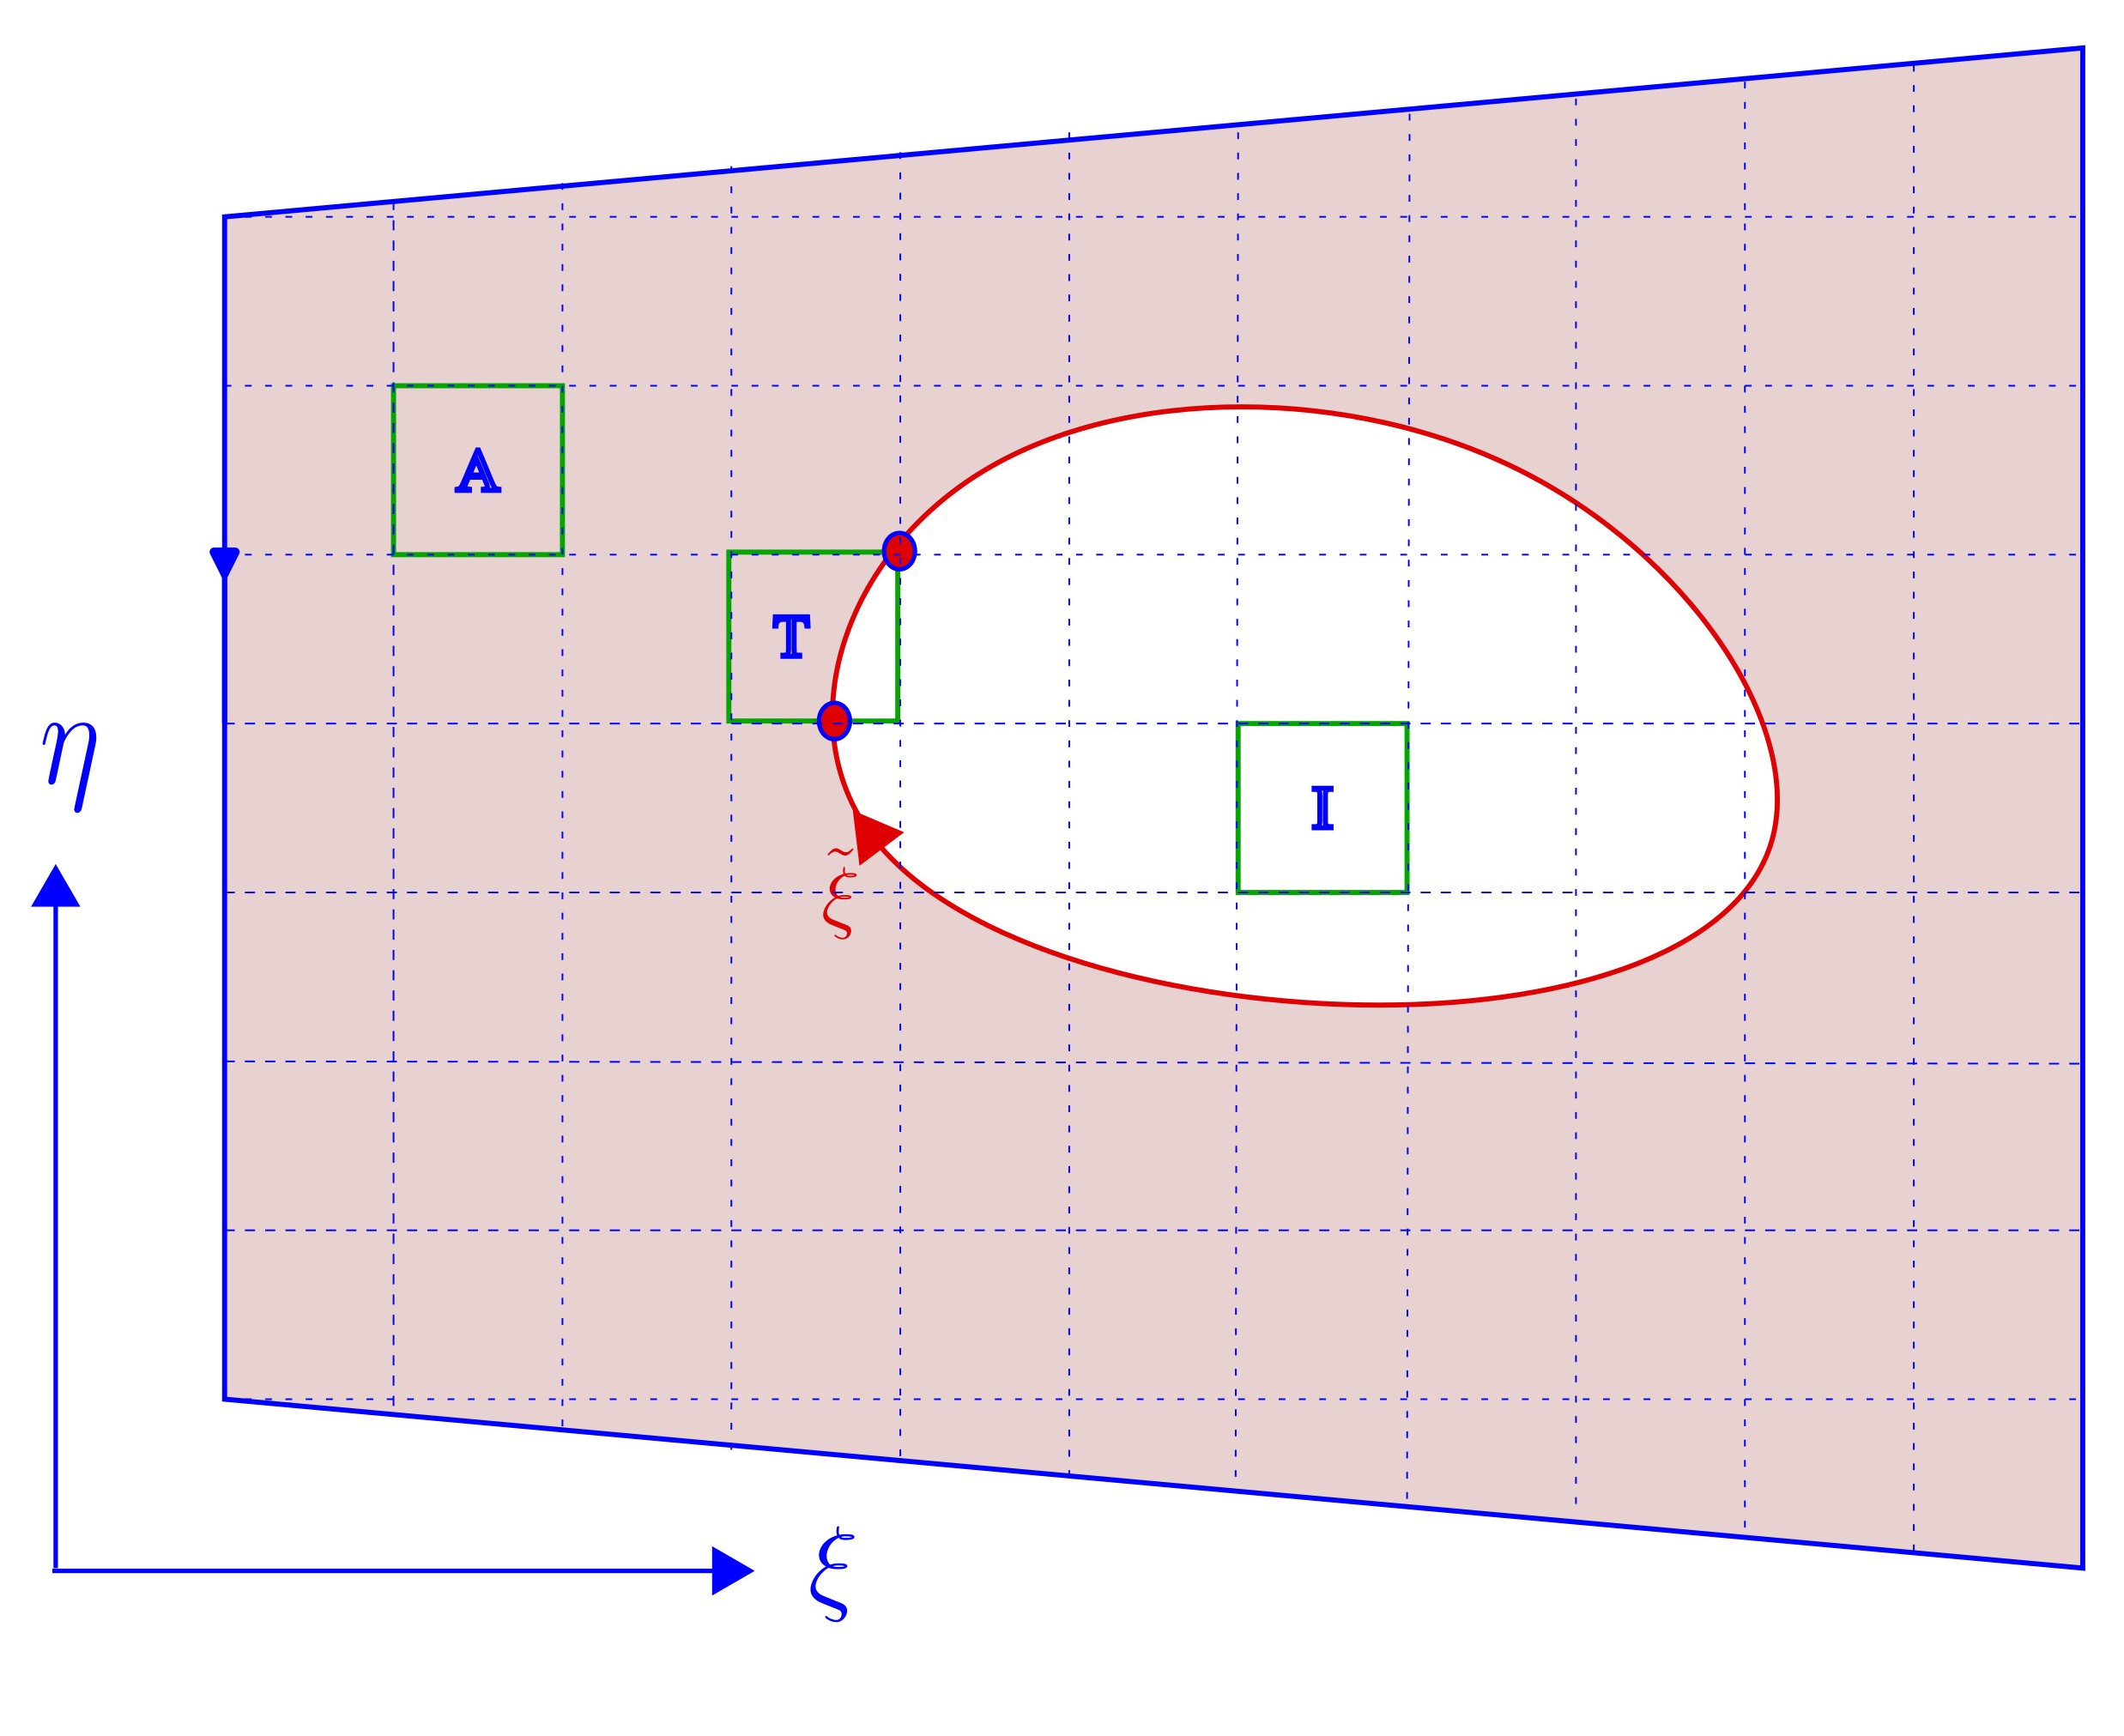
\includegraphics[width=0.6\textwidth]{Images/trim_active.jpg}
\caption{Active, trimmed and Inactive elements}
\label{fig:trim_el_type}
\end{figure}
\par Inactive elements are those which are completely within the domain of the trimming curve loop (element $\mathbf{I}$ in figure \ref{fig:trim_el_type}). There will be no contribution to the global stiffness matrix from this element. While the active elements of type $\mathbf{A}$ and trimmed elements 
 of type $\mathbf{T}$ will have a contribution to global stiffness, the Gauss points of trimmed elements will be modified and shifted so that only the untrimmed part of that element is considered. In the following subsections, two main methods for the analysis of trimmed elements is discussed.
 
\subsection{NURBS Enhanced Triangles}
This method \cite{trim_element_iga} proceeds by dividing the trimmed elements into normal triangles $R_{\triangle}$ and NURBS curved triangles $N_{\triangle}$ (meaning that one side of the triangle is part of the trimming curve) as shown in figure \ref{fig:NURBS_ENHANCED_TRIANGLE}
\begin{figure}[H]
\centering
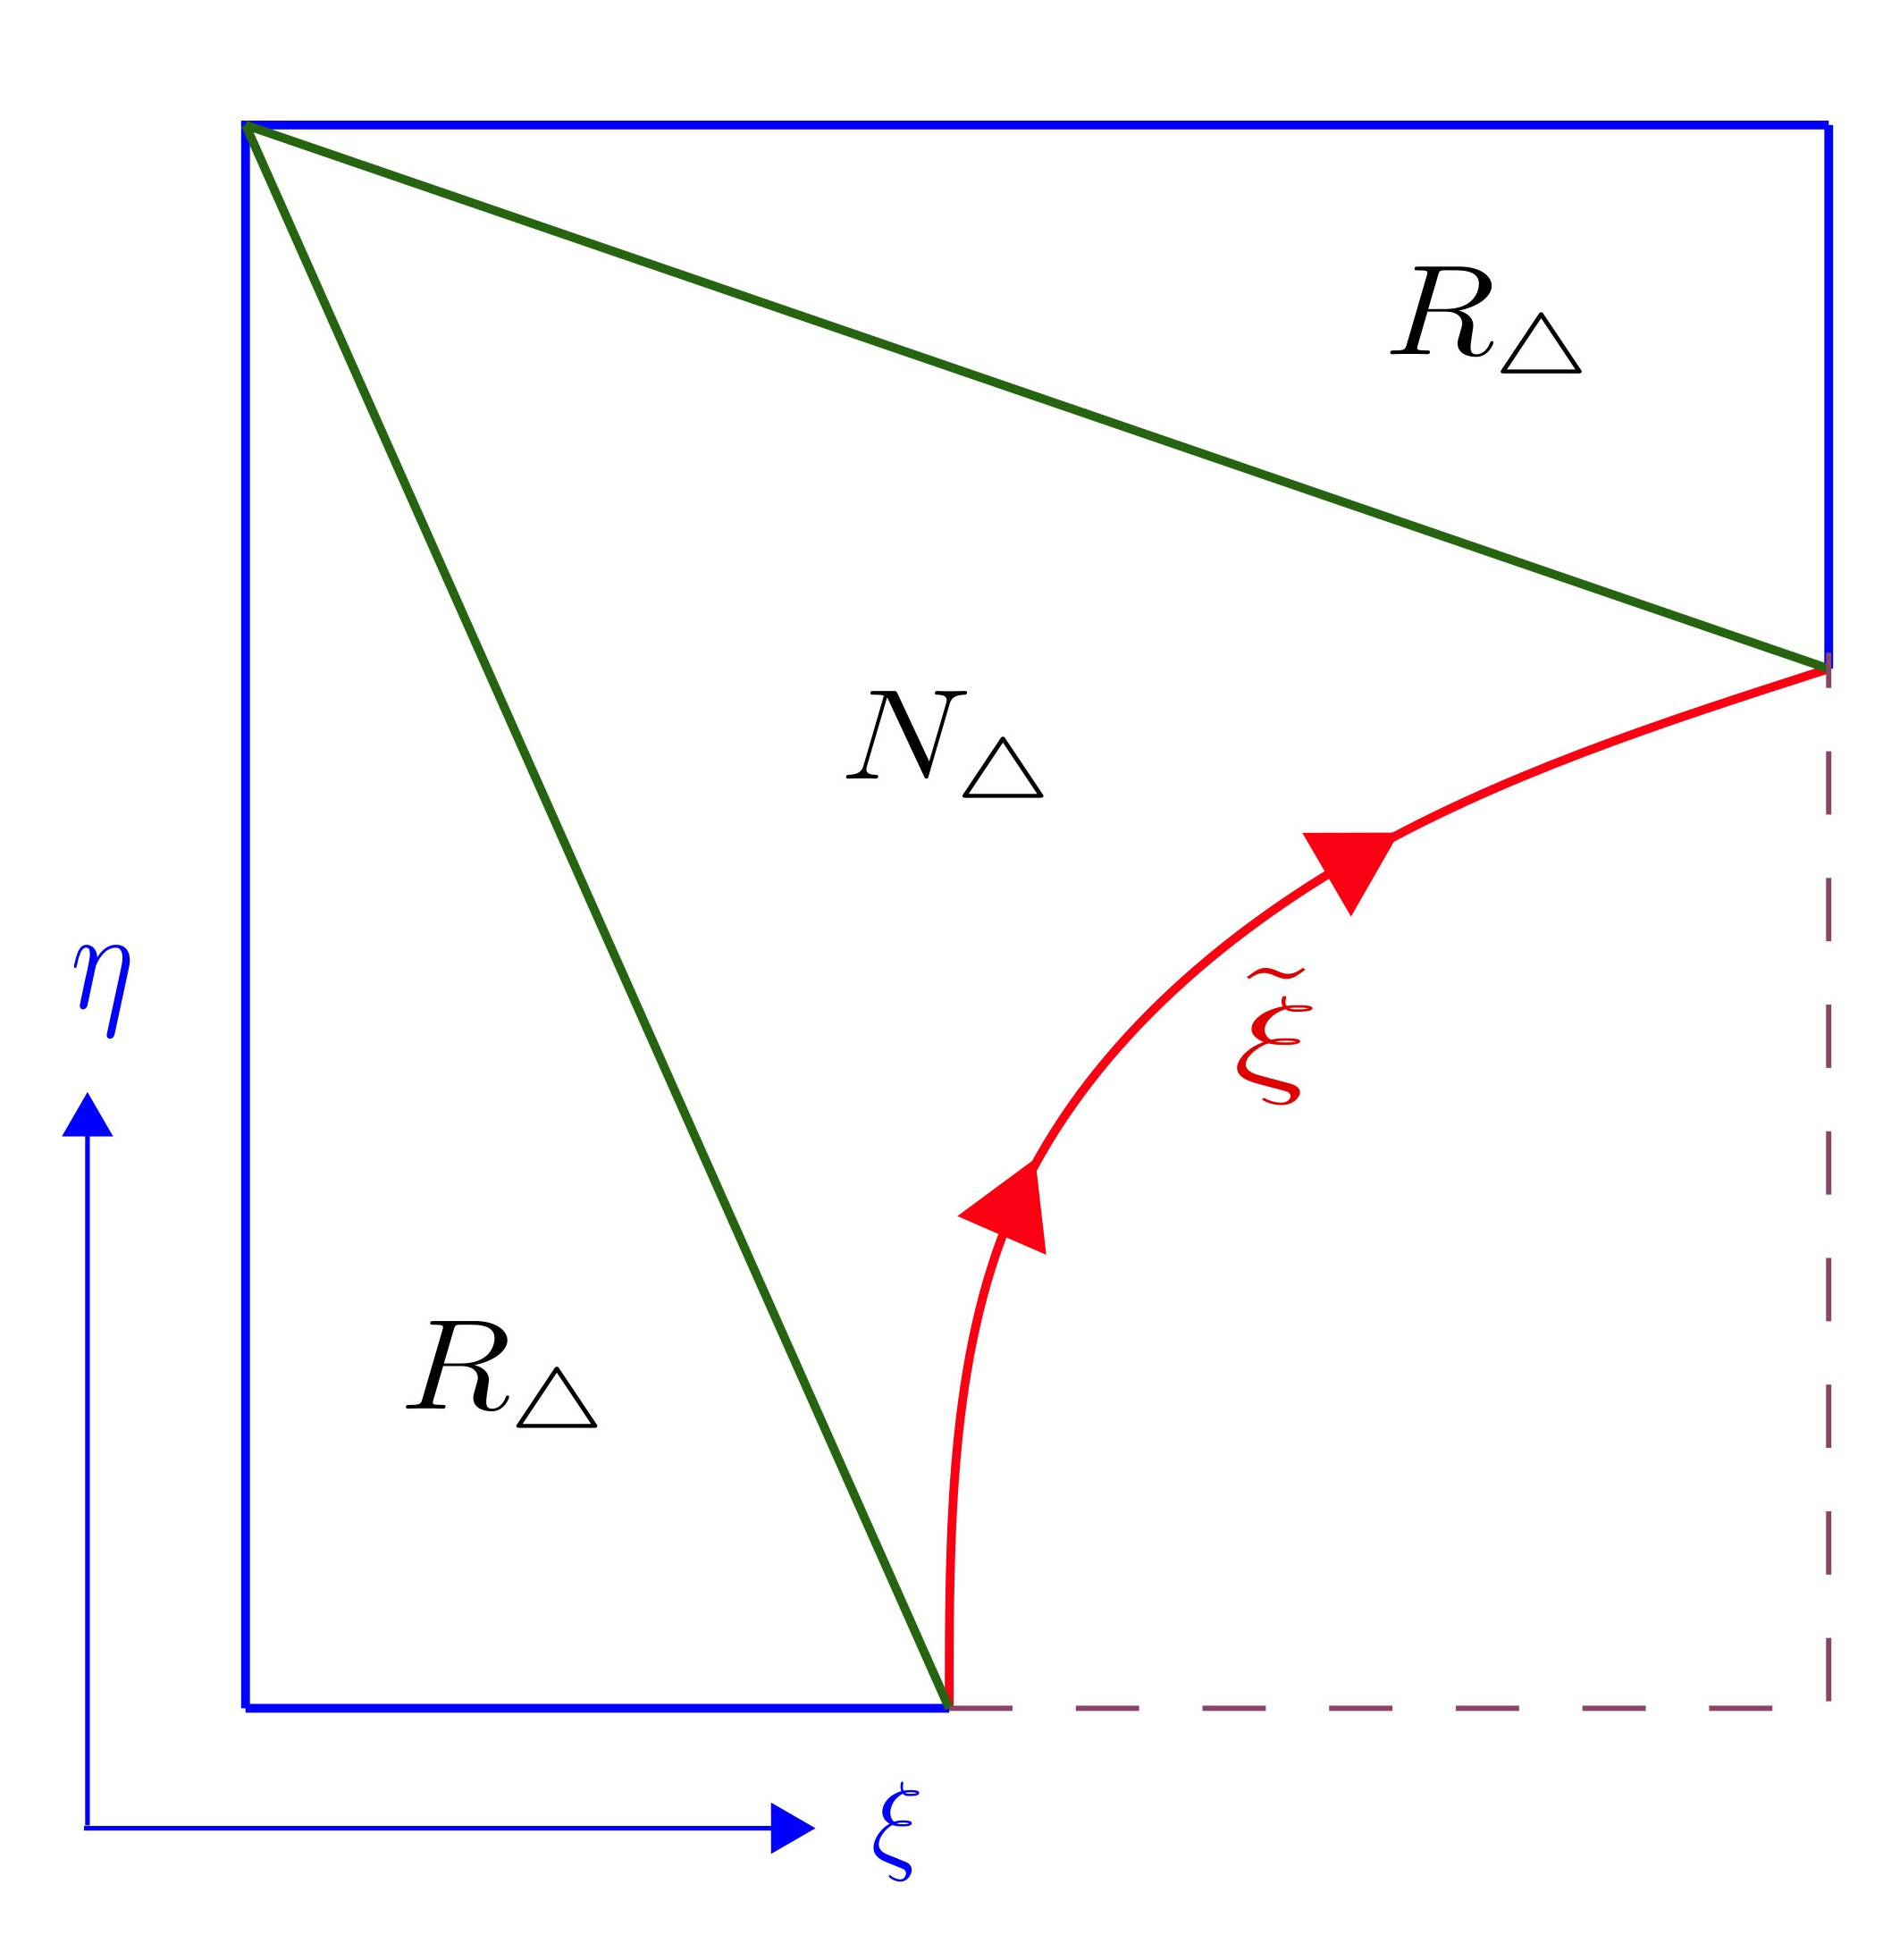
\includegraphics[width=0.4\textwidth]{Images/nurbs_en_tri.jpg}
\caption{Trimmed element divided into Triangles }
\label{fig:NURBS_ENHANCED_TRIANGLE}
\end{figure}
\subsubsection{Normal Triangular Elements $\boldsymbol{R_{\triangle}}$}
Normal triangular elements \cite{trim_element_iga_normal} are integrated using Gauss quadrature points for triangles followed by a mapping from the triangular Gaussian space to a triangle $R_{\triangle}$ in parametric space.
\begin{figure}[H]
\centering
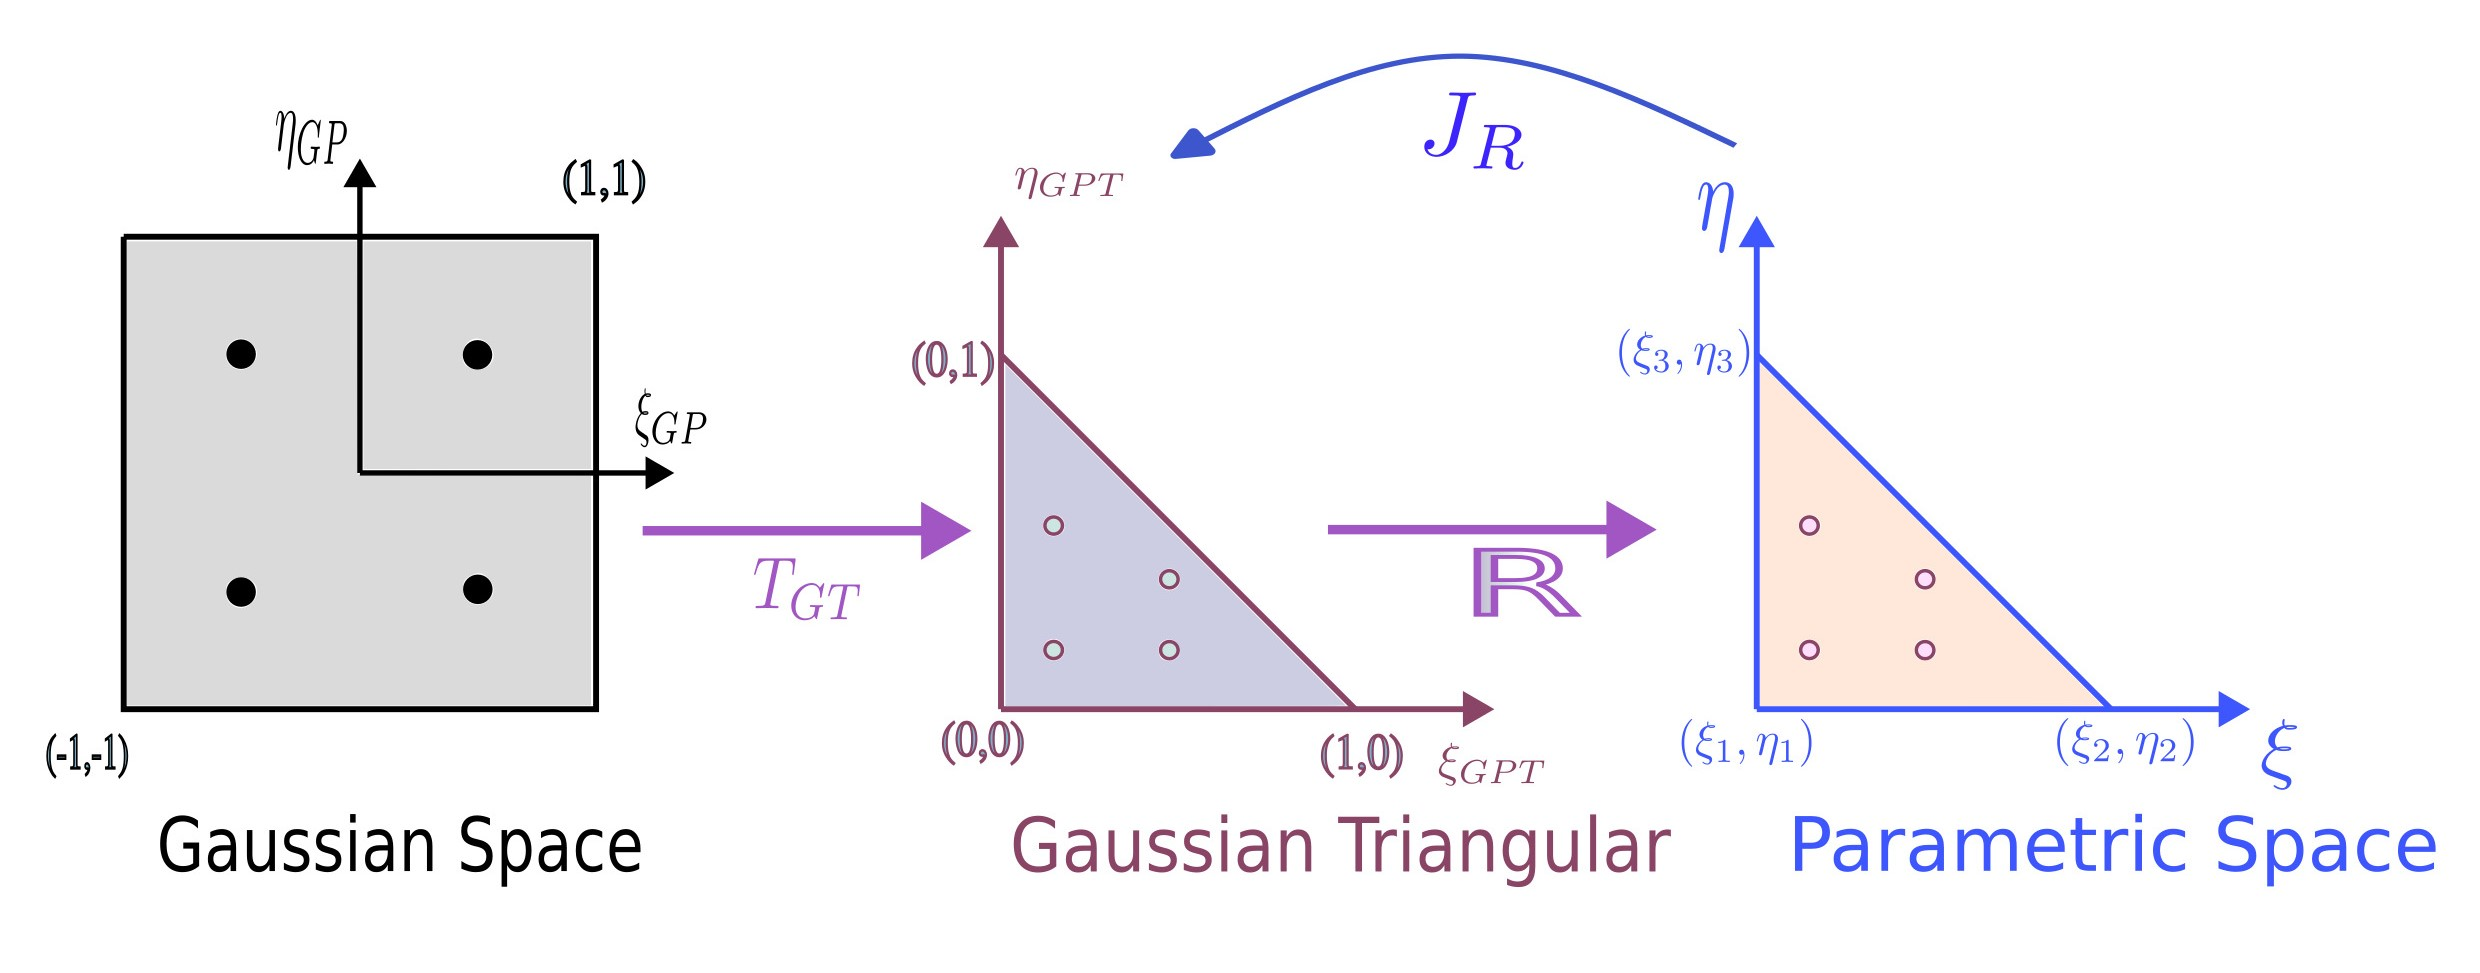
\includegraphics[width=0.8\textwidth]{Images/gauss_triangle_trans.jpg}
\caption{Transformation of spaces for normal triangular elements}
\label{fig:Gauss_TRIANGLES}
\end{figure}
The transformation $T_{GT}$ shown in figure \ref{fig:Gauss_TRIANGLES} expresses Gauss triangular points in terms of normal Gauss points as:
\begin{align}
    \xi_{GP,l} &= \frac{(1+\xi_i)}{2} \\
    \eta_{GP,l} &= \frac{(1-\xi_i)(1+\eta_j)}{4} \\
    W_{GP,l} &= \frac{(1-\xi_i)}{8}w_iw_j~~~i,j= 1,2.....,n_g 
\end{align}
The mapping $\boldsymbol{R}$ from Gaussian triangular space to  triangular parametric space is given by:
\begin{align}
    \begin{bmatrix}
    \xi \\
    \eta \\
  \end{bmatrix}
  &=
  \begin{bmatrix}
    (1-\xi_{GPT}-\eta_{GPT})*\xi_1 + \xi_{GPT}*\xi_2 + \eta_{GPT}*\xi_3 \\
    (1-\xi_{GPT}-\eta_{GPT})*\eta_1 + \xi_{GPT}*\eta_2 + \eta_{GPT}*\eta_3 \\
  \end{bmatrix}
\end{align}
And hence the Jacobian $J_R$ is given by:
\begin{equation}
  \boldsymbol{J_R}= \begin{bmatrix}    \frac{\partial \xi}{\partial \xi_{GPT}}& \frac{\partial \eta}{\partial \xi_{GPT}} \\
\frac{\partial \xi}{\partial \eta_{GPT}} &\frac{\partial \eta}{\partial \eta_{GPT}} \\\end{bmatrix}=\begin{bmatrix}    -\xi_1 + \xi_2& - \eta_1 + \eta_2 \\
 -\xi_1 + \xi_3 &- \eta_1 + \eta_3 \\\end{bmatrix}
\end{equation}
Based on the above discussion, the area of of a trimmed element for normal triangular elements can be calculated as:
\begin{equation}
  \left| \boldsymbol{\Omega} \right| \approx \sum_{l=1}^{n_g} \left| \boldsymbol{J_1}(\xi, \eta) \right| \left| \boldsymbol{J_{R}}(\xi_{GPT}, \eta_{GPT}) \right| W_{GPT}
\end{equation}
where the Jacobian $J_1$ from physical to parametric space as defined in section \ref{sec: iga_ele_integration}



\subsubsection{NURBS Enhanced Triangular Elements $\boldsymbol{N_{\triangle}}$}
Following mappings are needed (see figure \ref{fig:Gauss_TRIANGLES_2}):
\begin{itemize}[label=$\ast$]
  \item Mapping $\boldsymbol{P}$: From Gaussian space to a quadrilateral space $\boldsymbol{\Psi_e}$ where the axis $\boldsymbol{u}$ and $\boldsymbol{z}$ vary from [$u_1$,$u_2$] and [0,1] respectively and [$u_1$,$u_2$] being the intersection points between the trimming curve and the element.
  \item Mapping $\boldsymbol{Q}$:From $\boldsymbol{\Psi_e}$ to a triangular space $\boldsymbol{T_e}$ with axis ranging from 0 to 1.
  \item Mapping $\boldsymbol{R}$: From $\boldsymbol{T_e}$ to triangular sub-element in parametric domain.
\end{itemize}
\begin{figure}[H]
\centering
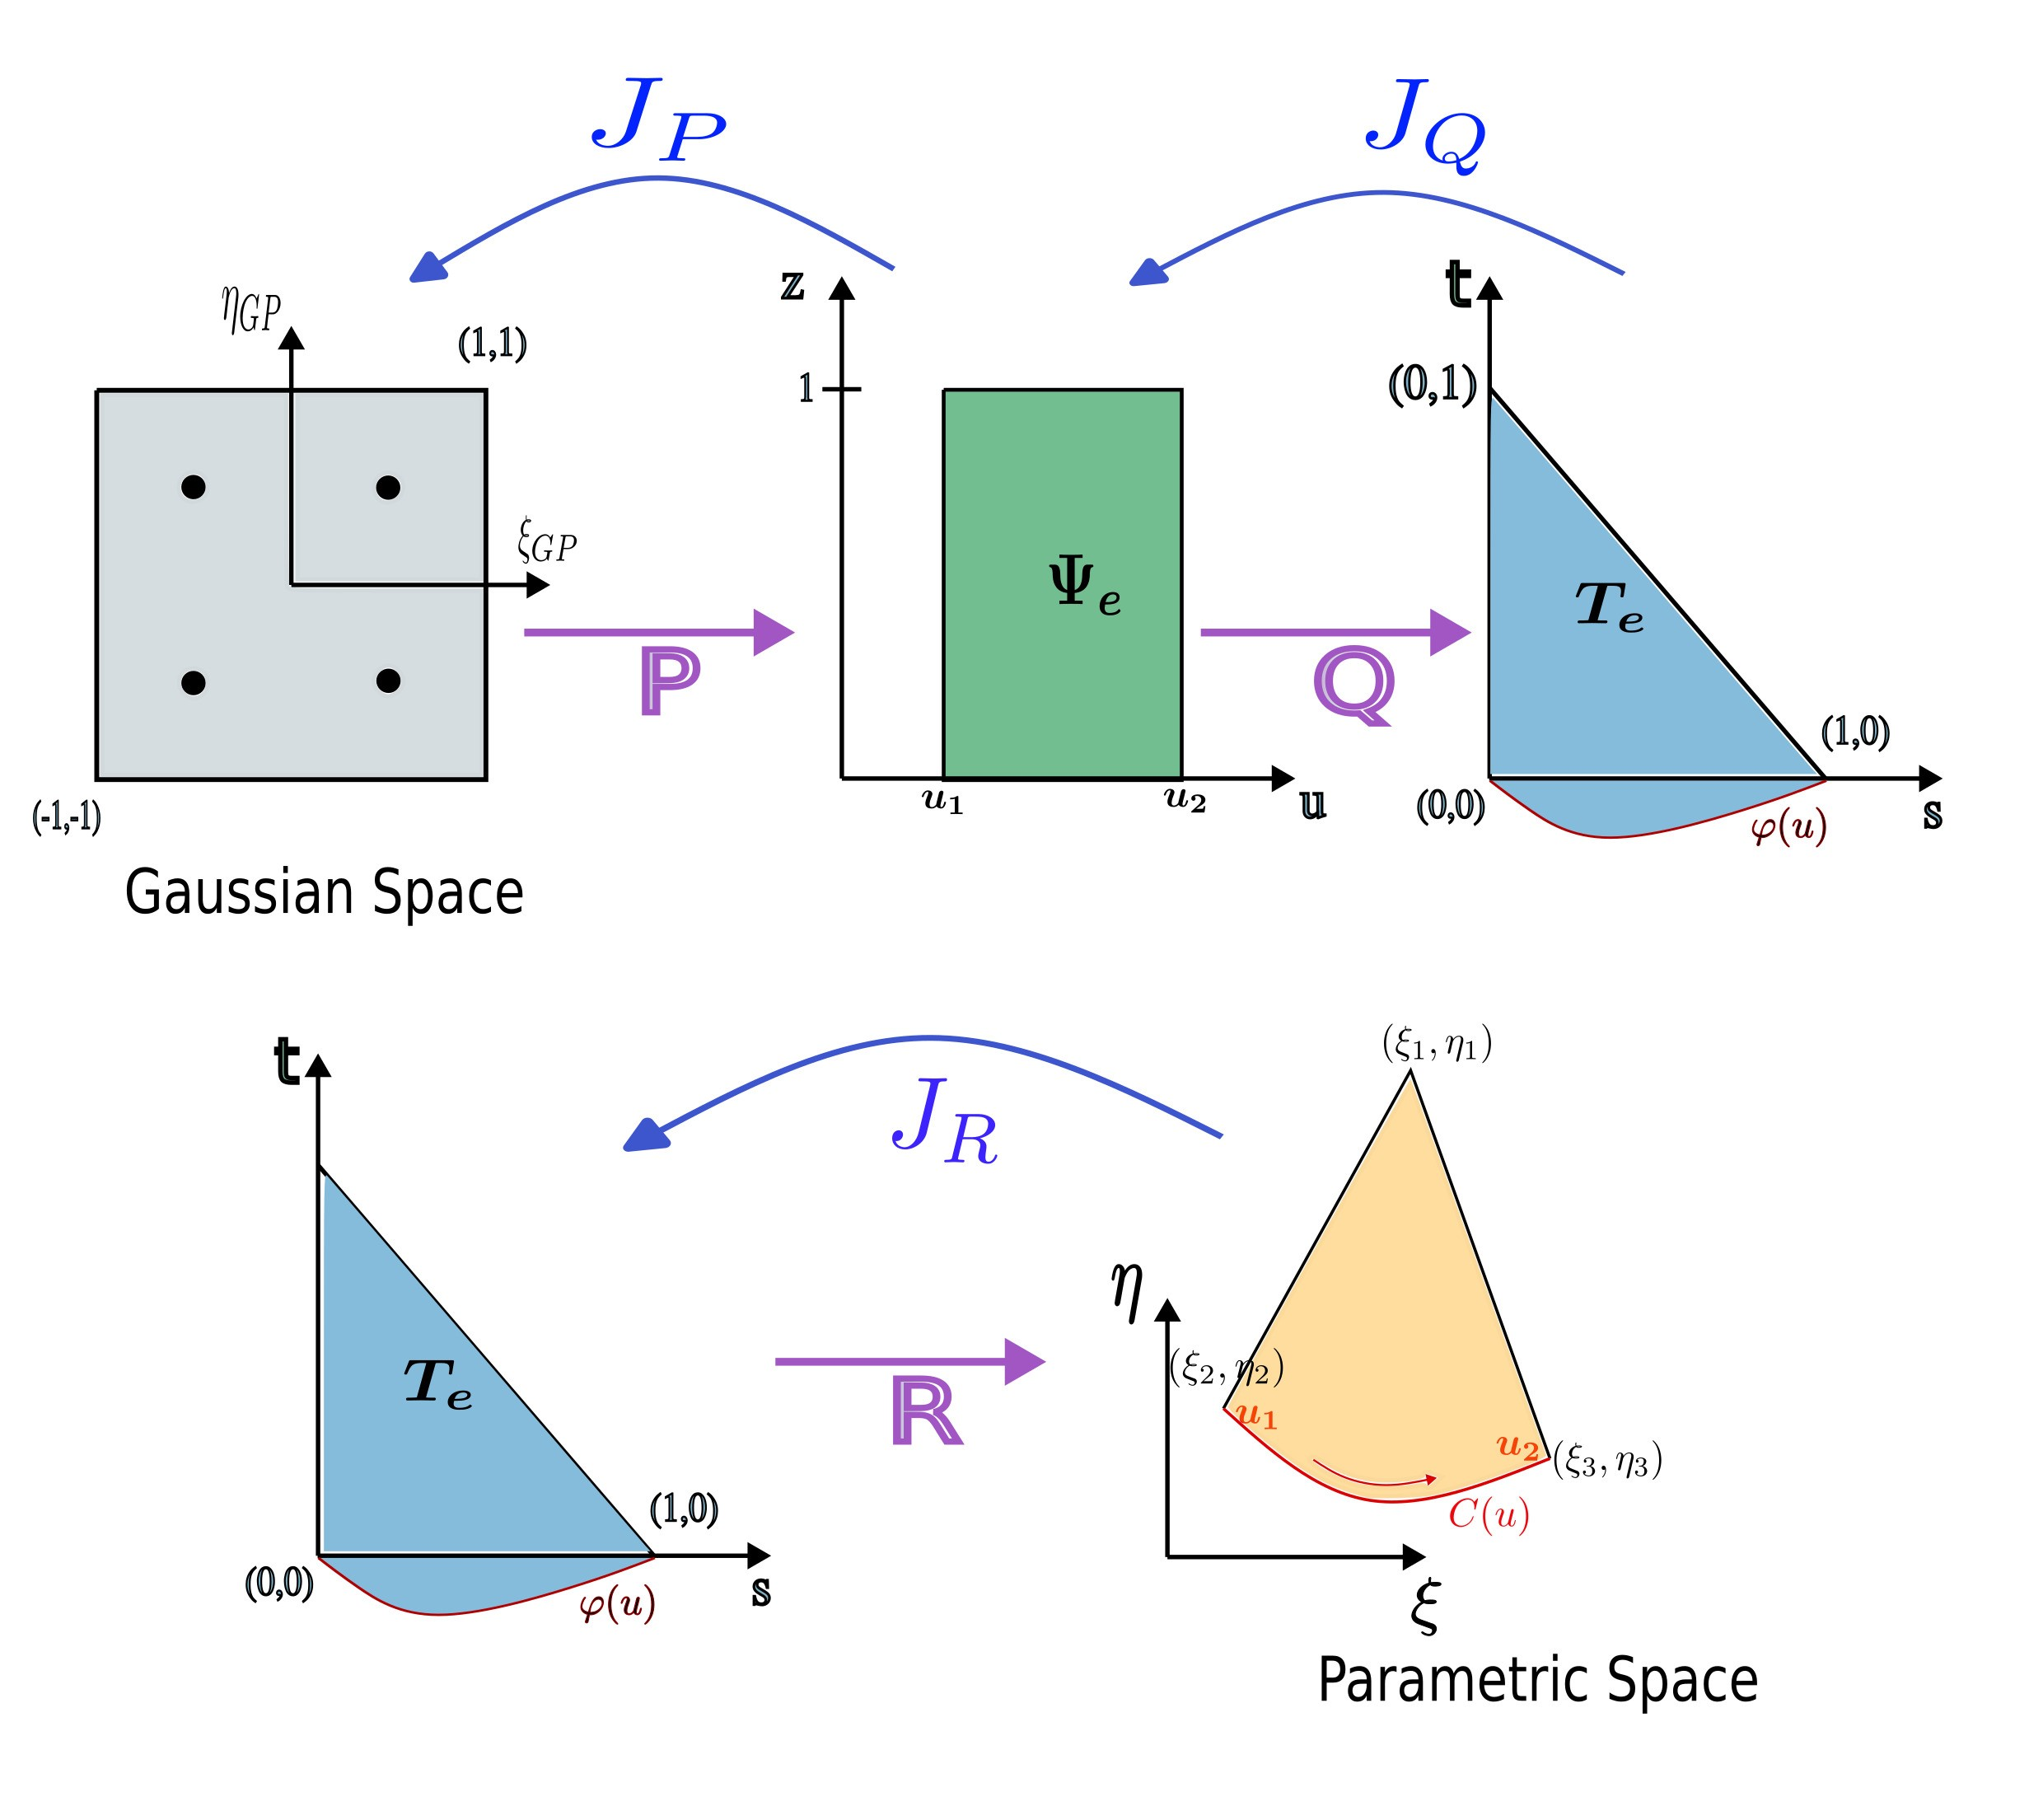
\includegraphics[width=0.8\textwidth]{Images/gauss_triangle_trans_2.jpg}
\caption{Transformation of spaces for NURBS enhanced triangular elements}
\label{fig:Gauss_TRIANGLES_2}
\end{figure}
The mapping P can be mathematically defined as:
\begin{align}
    \begin{bmatrix}
    u \\
    z \\
  \end{bmatrix}
  &=
  \begin{bmatrix}
    \frac{\xi_{GP}}{2}(u_2-u_1) + \frac{1}{2}(u_2+u_1) \\
    \frac{\eta_{GP}}{2} + \frac{1}{2} \\
  \end{bmatrix}
\end{align}

And its Jacobian as:
\begin{equation}
  \boldsymbol{J_P}= \begin{bmatrix}    \frac{\partial u}{\partial \xi_{GP}}& \frac{\partial z}{\partial \xi_{GP}} \\
\frac{\partial u}{\partial \eta_{GP}} &\frac{\partial z}{\partial \eta_{GP}} \\\end{bmatrix}=\begin{bmatrix}    \frac{u_2-u_1}{2}& 0 \\
 0 & \frac{1}{2} \\\end{bmatrix}
\end{equation}

Likewise for mapping $\boldsymbol{Q}$:
\begin{align}
  \begin{bmatrix}
    s \\
    t \\
  \end{bmatrix}
  &=
  \begin{bmatrix}
    \varphi_s(u)(1-z) \\
    \varphi_t(u)(1-z) + z \\
  \end{bmatrix} \\
  \boldsymbol{J_Q} &=
  \begin{bmatrix}
    \frac{\partial s}{\partial u} & \frac{\partial t}{\partial u} \\
    \frac{\partial s}{\partial z} & \frac{\partial t}{z} \\
  \end{bmatrix} =
  \begin{bmatrix}
    \frac{u_2 - u_1}{2} & 0 \\
    0 & \frac{1}{2} \\
  \end{bmatrix}
\end{align}

Where:
\begin{equation}
   \varphi(u) = 
\begin{bmatrix}
  \varphi_s(u) \\
    \varphi_t(u) \\    
\end{bmatrix} = [\boldsymbol{A_1}^{-1}] \left( \begin{bmatrix}
  C_{\xi}(u) \\
  C_{\eta}(u) \\    
\end{bmatrix} - [\boldsymbol{A_2}] \right)
\end{equation}

\begin{align}
\boldsymbol{A_1} &= \begin{bmatrix}
    \xi_3-\xi_2 & \xi_1-\xi_2 \\
    \eta_3-\eta_2 & \eta_1-\eta_2\\
\end{bmatrix}\\
 \boldsymbol{A_2} &= \begin{bmatrix}
    \xi_2 \\
    \eta_2 \\
\end{bmatrix}
\end{align}


And mapping $\boldsymbol{R}$:
\begin{align}
  \begin{bmatrix}
    \xi \\
    \eta \\
  \end{bmatrix}
  &=
  \begin{bmatrix}
    (t)\xi_1 + (1-s-t)\xi_2 + (s)\xi_3 \\
    (t)\eta_1 + (1-s-t)\eta_2 + (s)\eta_3 \\ \\
  \end{bmatrix} \\
  \boldsymbol{J_R} &=
  \begin{bmatrix}
    \frac{\partial \xi}{\partial s} & \frac{\partial \eta}{\partial s} \\
    \frac{\partial \xi}{\partial t} & \frac{\partial \eta}{t} \\
  \end{bmatrix} =
  \begin{bmatrix}
    -\xi_2+\xi_3\ & -\eta_2+\eta_3 \\
    \xi_1-\xi_2\ & \eta_1-\eta_2 \\
  \end{bmatrix}
\end{align}
The determinant of the overall combined Jacobian of the mappings can be defined as:
\begin{equation}
    |\boldsymbol{J_C}|= |\boldsymbol{J_P}|.|\boldsymbol{J_Q}|.|\boldsymbol{J_R}|
\end{equation}
The area of the triangle can be evaluated as:
\begin{equation}
  \left| \boldsymbol{\Omega} \right| \approx \sum_{l=1}^{n_g} \left| \boldsymbol{J_1}(\xi, \eta) \right| \left| \boldsymbol{J_{C}} \right|W~~~,W=w_iw_j
\end{equation}
where the Jacobian $J_1$ from physical to parametric space as defined in section \ref{sec: iga_ele_integration}



\subsection{Adaptive Gaussian integration}
The idea of this approach is to construct an untrimmed surface $\boldsymbol{\tilde{S}}$ inside the Gaussian space. This surface is then used to distribute the Gauss quadrature points (see figure \ref{fig:AGIP}). To create this surface, the trimming curve is scaled, shifted and rotated so that it fits the Gaussian space and that only the height of the element varies. In-depth details of the method can be found in \cite{AGIP}. Further discussion about this method is out of the scope of the current thesis.
\textbf{\begin{figure}[H]
\centering
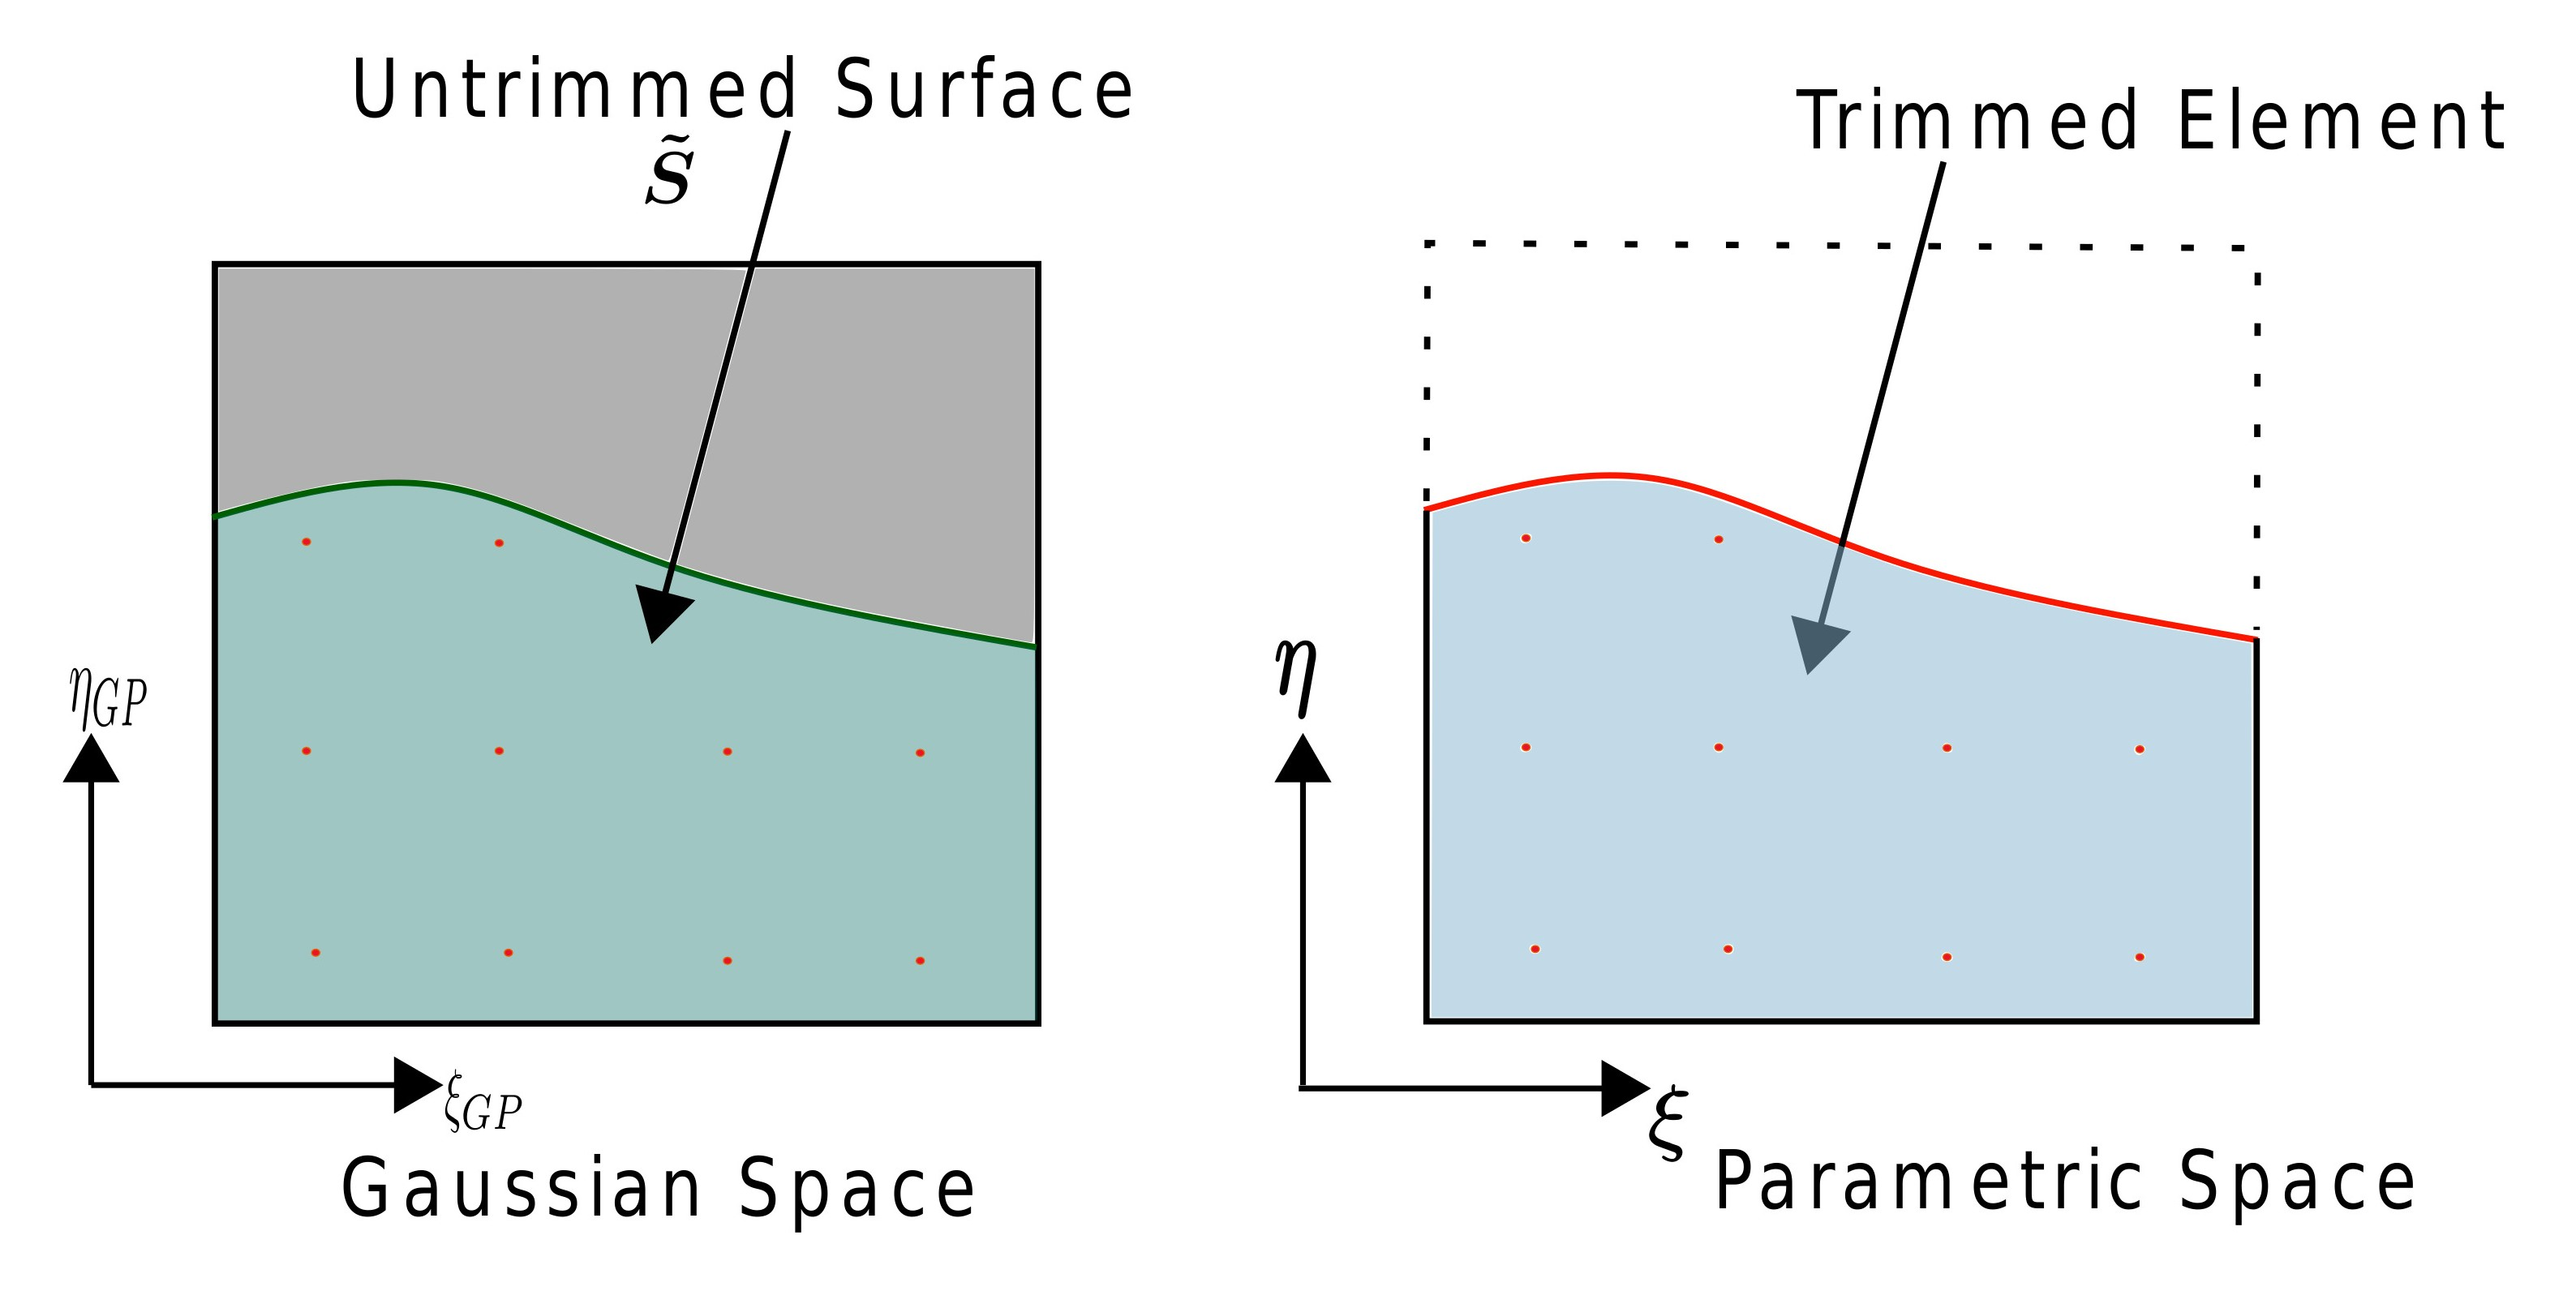
\includegraphics[width=0.8\textwidth]{Images/AGIP.jpg}
\caption{Distribution of Gauss points in Gaussian and Parametric spaces}
\label{fig:AGIP}
\end{figure}}

\section{IGA of Rectangular plate with a circular hole in the App}
\subsection{Visualization and Trimmed Data}
For the visualization of trimmed geometries in MATLAB with the application of PythonOCC, the representation of the trimming curve ($\tilde{\xi}$) in the parametric space of the rectangular NURBS surface is obtained and an array of points on the curve ($\xi,\eta$) are obtained and parsed from the python script to MATLAB along with the usual details of a NURBS surface (refer to  Appendix A3 [\ref{app Appendix_A3_trimPlate}] for details). \newline

\begin{figure}[H]
\centering
\begin{subfigure}{.5\textwidth}
  \centering
  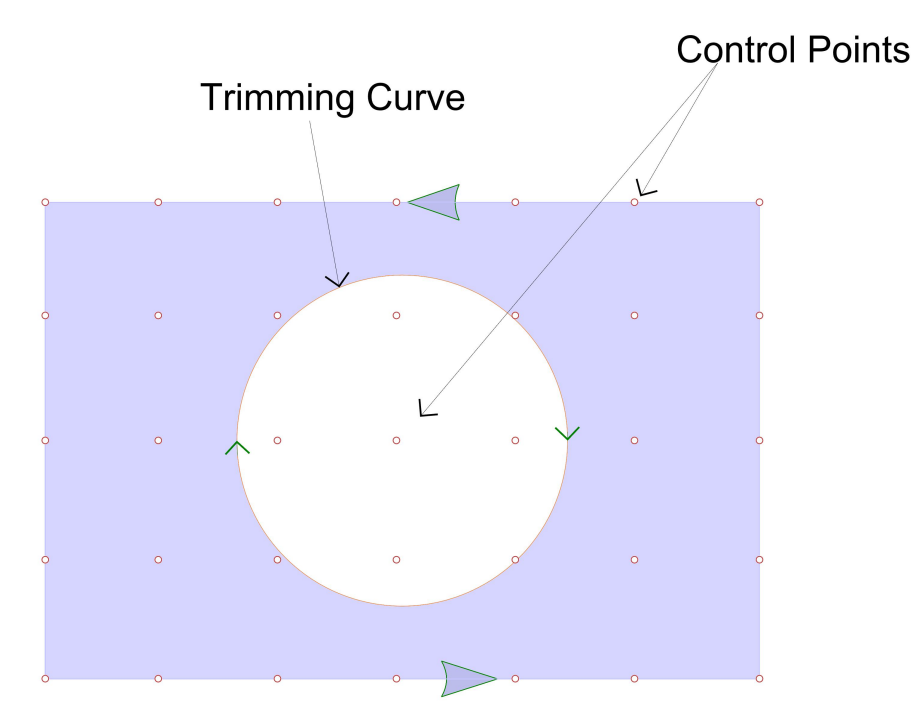
\includegraphics[width=0.9\linewidth]{Images/trimDemo.png}
  \caption{Trimming curve orientation}
  \label{fig:tSurf}
\end{subfigure}%
\begin{subfigure}{.5\textwidth}
  \centering
  \includegraphics[width=0.9\linewidth]{Images/delaunay_mesh_element.jpg}
  \caption{Delaunay Meshing of trimmed element}
  \label{fig:Delaunay}
\end{subfigure}
\caption{Trimmed Plate }
\label{fig:trimmed plate}
\end{figure}
\subsection{Element creation and Delaunay Triangulation} Once the data is available in MATLAB, a polygon ($\textbf{\textit{polyshape}}$ in MATLAB) is created using the parsed points of the curve to approximate it.  For the analysis, each element is represented by a rectangle (($\textbf{\textit{polyshape}}$) with four vertices as the knot bounds in two directions. The set-up is explained in Figure \ref{fig:Delaunay}. When the element intersects with the curve, the intersecting points are captured using MATLAB $\textbf{\textit{intersect}}$ command. Then the portion of the element outside the curve is triangulated using $\textbf{\textit{Delaunay}}$ triangulation. As can be seen in the figure, the trimmed element is approximated by three triangles. Gauss points are obtained on each triangle after proper transformations (see section \ref{subsection: methods_trim_iga})\par
\textbf{Note on Intersection:} For practical analysis, since the plate is very well refined in both the directions, the approximation error because of the triangulation is not significant. For better results, the enhanced-NURBS triangle method can also be fully implemented with one side as a NURBS curve to increase accuracy. Also, linearization of the trimming curve can also be avoided and a high level algorithm implemented to to find intersection of the isoparametric curves of the surface with the trimming curve, as is already done in this thesis for implemented weak Dirichlet boundary conditions as well as coupling conditions.
\vspace{-10pt}


\begin{figure}[H]
\centering
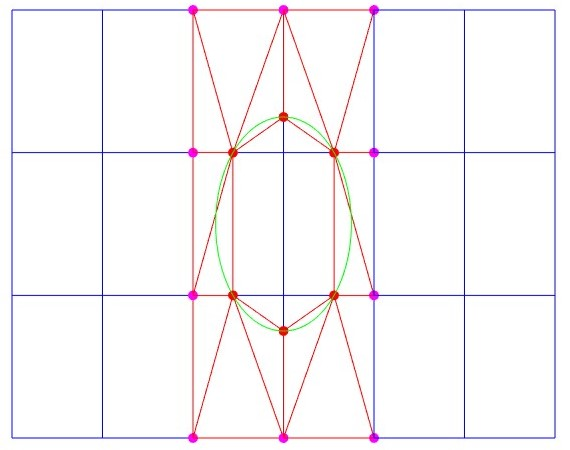
\includegraphics[width=0.6\textwidth]{Images/trim_rect_mesh_triangles.jpg}
\caption{Delaunay meshing (very coarse for demonstration only) of all trimmed elements}
\label{fig:trim_rect_delaunay}
\end{figure}
The rest of the analysis procedure is the same except that the element stiffness matrix of those elements which are completely within the trimming curve is not computed and hence not assembled in the global stiffness matrix.Thus the entries of the global stiffness matrix corresponding to the inactive degrees of freedom are all zeroes.

\chapter{IGA of multi-patch geometries} \label{chap: Multipatch IGA}
Just like CAD geometries of complex real life physical objects are almost always trimmed, in the same manner they are also composed of many individual NURBS patches, hence the name multi-patch. These patches may or may not have the same parametrizations depending not only on the way how the individual patches are created but also on how they are refined. //figure shows a two path geometry. In the following sections, some popular methods for the imposition of Dirichlet boundary conditions are introduced. Without the loss of generality, theses have also been used for the coupling of adjacent patches.
\section{Coupling of multi-patches and weak imposition of Dirichlet Boundary conditions}
When the CAD geometry is modeled by multiple NURBS patches (which is usually the case), continuity constraints have to be imposed on their interfaces and boundaries in order to perform meaningful simulations.
This might include displacement and/or rotational continuity along the interfaces and imposition of Dirichlet conditions along the boundaries depending upon the analysis formulation applied.
\begin{align}
    u^{(1)}- u^{(2)} &= 0 ~~\forall ~x \in \Gamma_c \\
    \phi^{(1)}- \phi^{(2)} &= 0 ~~\forall ~x \in \Gamma_c 
 \end{align}

The essential boundary conditions for a plate or a shell are expressed in terms of mid-surface displacements $u$ and rotations $\phi$ as:
\begin{align}
    u- \bar{u} &= 0 ~~\forall ~x \in \Gamma_d \\
    \phi- \bar{\phi} &= 0 ~~\forall ~x \in \Gamma_d 
 \end{align}
 where $\bar{u}$ and $\bar{\phi}$ are respectively the prescribed displacements and rotations along the Dirichlet boundary $\Gamma_d$
\subsection{Direct Method}
Because of the non-interpolating nature of the NURBS basis functions, due to which Kronecker Delta like behaviour cannot be produced, a different way of imposing the essential boundary conditions has to be implemented. This need was first identified by \cite{HUGHES20054135} where they imposed the essential boundary conditions directly on the control points at their spatial locations. This method also known as the Direct Method (DM) doesn't give reliable results in case of non-homogenous boundary conditions. Also if the control points are not located on the exact boundary (for which there is no guarantee), enforcing boundary values on the control points is not physically meaningful. There have been several efforts aimed at the proper imposition of essential boundary conditions.
\subsection{Transformation Method}
\par One method called the Transformation Method (TM) proposed by \cite{WANG20102425} is also based on separation of control points into interior and boundary control points by repeating the knots at the end of knot vectors to vanish the corresponding NURBS basis functions associated with the interior control points vanish at the boundary. The transformation method links control variables to their corresponding values on the physical boundary to accurately impose the boundary conditions. Although it produces better results than the DM, it can result in singular transformation matrix.

\subsection{Lagrange Multiplier Method} Shortly after that, the usage of the Lagrange Multiplier method for the imposition of Dirichlet boundary conditions was proposed by \cite{lagDBC}. As demonstrated, this method is capable of modeling incomplete Dirichlet boundaries. the variational problem (ignoring the rotations and moments, without the loss of generality) of minimizing the total potential energy functional results in:
\begin{equation}
   \textbf{minimize}: \frac{1}{2} t \int_{\Omega} \varepsilon^T \sigma d \Omega -\int_{\Gamma_N} u^T f_t d \Gamma-\sum_{i=1}^m \int_{\Gamma_{D_i}} \lambda_i\left(u-\bar{u}_i\right) d \Gamma
\end{equation}
where the first term corresponds to the strain energy of the system, the second to the work done by the traction forces (assuming no body forces), $u$ is the degrees of freedom (vector), $\bar{u_i}$ is the known value of displacement on the Dirichlet boundary $\Gamma_{D_i}$, $t$ is the thickness of the plate/shell, $m$ is the number of Dirichlet boundaries, $\lambda_i$ is the Lagrange multiplier vector corresponding to $\Gamma_{D_i}$
\begin{equation}
{\left[\begin{array}{cc}
K & G \\
G^T & 0
\end{array}\right]\left\{\begin{array}{l}
d \\
\lambda
\end{array}\right\}=\left\{\begin{array}{l}
f \\
q
\end{array}\right\}} \\
\end{equation}

\begin{equation}
K=\int_{\Omega} B^T D B d \Omega \\
\end{equation}

where $q_i = \int_{\Gamma_{D_i}} N_i^T \bar{u_i}d \Gamma$ , $G_i=\int_{\Gamma_{D_i}} R^T N_i d \Gamma$ and $f= \int_{\Gamma_{D_N}} R^T f_t d \Gamma$
\subsection{Penalty Method}
If we derive the variational form using the virtual work principle, the following penalty virtual work is introduced:
\begin{equation}\label{eq: pen_DBC}
    \delta W^{p} = \int_{\Gamma_{d}} \alpha (u-\bar{u})\delta u \,d\Gamma
\end{equation}
\par
Penalty method has been implemented in the current thesis both for the imposition of Dirichlet boundary (see equation \ref{eq: pen_DBC}) conditions as well as coupling of multi-patches (see equations \ref{eq: pen_coupling_1} and \ref{eq: pen_coupling_2} ) along a common interface (edge or a trimming curve). The continuity constraints on the interfaces can be obtained by augmenting the virtual work expression by two penalty terms. These include virtual work terms for the force and moment equilibrium along the boundary of two patches, expressed as\cite{BREITENBERGER2015401}:
\begin{align}\label{eq: pen_coupling_1}
    \delta W^{u} &= -\alpha_{\text {u}} \int_{\Gamma_{\mathrm{c}}^{(1)}}\left(\mathbf{u}^{(1)}-\mathbf{u}^{(2)}\right)\left(\delta \mathbf{u}^{(1)}-\delta \mathbf{u}^{(2)}\right) \mathrm{d} \Gamma_{\mathrm{}}^{(1)}
    \\\label{eq: pen_coupling_2}
    \delta W^{\phi} &= -\alpha_{\phi} \int_{\Gamma_{\mathrm{c}}^{(1)}}\left(\boldsymbol{\phi}^{(1)}\pm \boldsymbol{\phi}^{(2)}\right)\left(\delta \boldsymbol{\phi}^{(1)}\pm \delta \boldsymbol{\phi}^{(2)}\right) \mathrm{d} \Gamma_{\mathrm{}}^{(1)}
\end{align}
where $\alpha_{\text {u}}$ and $\alpha_{\phi}$ are the penalty factors for the displacements and rotations. These are controlled by a single dimensionless parameter $\alpha$ given as \cite{jos_kind_shell_penalty}:
\begin{align}
    \alpha_u&=\alpha \frac{Et}{h(1-\nu^2)}\\
    \alpha_{\phi}&=\alpha \frac{Et^3}{12h(1-\nu^2)}\\
\end{align}
where $E$ is the Young's modulus, $\nu$ the Poisson's ratio, $t$ the thickness of the plate/shell and $h$ the average element length in $\Gamma_c$
The tangential coupling stiffness matrices are therefore given as:
\begin{align}\label{eq:coupling_stiff_1}
    K_{r s}^{u} &= \alpha_{\mathrm{u}} \int_{\Gamma_{\mathrm{c}}^{(1)}}\left(\mathbf{u}_{, s}^{(1)}-\mathbf{u}_{, s}^{(2)}\right) \cdot\left(\mathbf{u}_{, r}^{(1)}-\mathbf{u}_{, r}^{(2)}\right) \mathrm{d} \Gamma_{\mathrm{}}^{(1)} \\
    \begin{split}\label{eq:coupling_stiff_2}
    K_{r s}^{\phi} &= \alpha_{\mathrm{u}} \int_{\Gamma_{\mathrm{c}}^{(1)}}\left[\left(\phi_{\mathbf{T}_2, s}^{(1)} \pm \phi_{\mathbf{T}_2, s}^{(2)}\right)\left(\phi_{\mathbf{T}_2, r}^{(1)} \pm \phi_{\mathbf{T}_2, r}^{(2)}\right) \right. \\
    &\quad + \left. \left(\phi_{\mathbf{T}_2}^{(1)} \pm \phi_{\mathbf{T}_2}^{(2)}\right)\left(\phi_{\mathbf{T}_2, r s}^{(1)} \pm \phi_{\mathbf{T}_2, r s}^{(2)}\right)\right] \mathrm{d} \Gamma_{\mathrm{}}^{(1)}
    \end{split}
\end{align}
where $\mathbf{T_2}$ is the tangent vector along the boundary and r,s are the discretization parameters.\par
For the sake of completion, one might be interested in knowing that many more methods have been studied and implemented like the reduced Lagrange Multiplier method \cite{Reduced_LM}, Nitsche's method \cite {Nitsch_DBC} etc for the weak imposition of boundary conditions.

\section{Implementation of Penalty Method for the coupling of RM plate patches}
Figure \ref{fig:patch_couple_1} shows two plane patches with different parametrizations modeled as Reissner-Mindlin plates to be coupled along a trimming curve. The following subsections are based on \cite{jos_kind_shell_penalty}


\subsection{Coupling curve in the physical space}
If $\mathbf{c(\tilde{\xi})}$ is the spatial description of the interface curve $\Gamma_c$, then the tangent vector is obtained as:
\begin{equation}
    \mathbf{T_2}=\frac{\partial \mathbf{c}}{\partial \tilde{\xi}}
\end{equation}
and the length of the elements along the curve can be computed as:
\begin{equation}\label{eq: pen_coup_curve_len_1}
    |L|=\int_{\Gamma_{c}} d\Gamma = \int_{\tilde{\xi_1}} \|\mathbf{T_2}\|d\tilde{\xi}
\end{equation}
As required in equations \ref{eq:coupling_stiff_1} and \ref{eq:coupling_stiff_2}, the tangent vector needs to be projected onto the surfaces in order to find variations with respect to the degrees of freedom (r,s) of the surfaces. So equation \ref{eq: pen_coup_curve_len_1} is evaluated as:
\begin{equation}
|L|=\int_{\Gamma_{\mathrm{c}}} d \Gamma_{\mathrm{}}=\int_{\tilde{\xi}}\left\|\frac{d \mathbf{X}_{\text {surf }}}{d \tilde{\xi}}\right\|_2 \mathrm{~d} \tilde{\xi}=\int_{\tilde{\xi_1}}\left\|\left(\frac{\partial \mathbf{X}_{\text {surf }}}{\partial \xi} \frac{d \xi}{d \tilde{\xi}}+\frac{\partial \mathbf{X}_{\text {surf }}}{\partial \eta} \frac{d \eta}{d \tilde{\xi}}\right)\right\|_2 \mathrm{~d} \tilde{\xi},
\end{equation}
\subsection{Point inversion and point projection: Element creation}
For evaluating integrals in equations \ref{eq:coupling_stiff_1} and \ref{eq:coupling_stiff_2}, the integration points defined in the parametric space of the coupling curve, are also needed in the parametric spaces of the patches. This process is called point inversion. In this thesis, it is accomplished using the available classes and algorithms provided in the \href{https://dev.opencascade.org/doc/refman/html/files.html}{OCCT library}. {for details  Refer to APPENDIX} As shown in figure \ref{fig:patch_couple_1}, the intersection points of the coupling curve with the secondary patch need to be transferred to the primary patch (on which the integration is performed) which is achieved by point projections. 


\textbf{\begin{figure}[H]
\centering
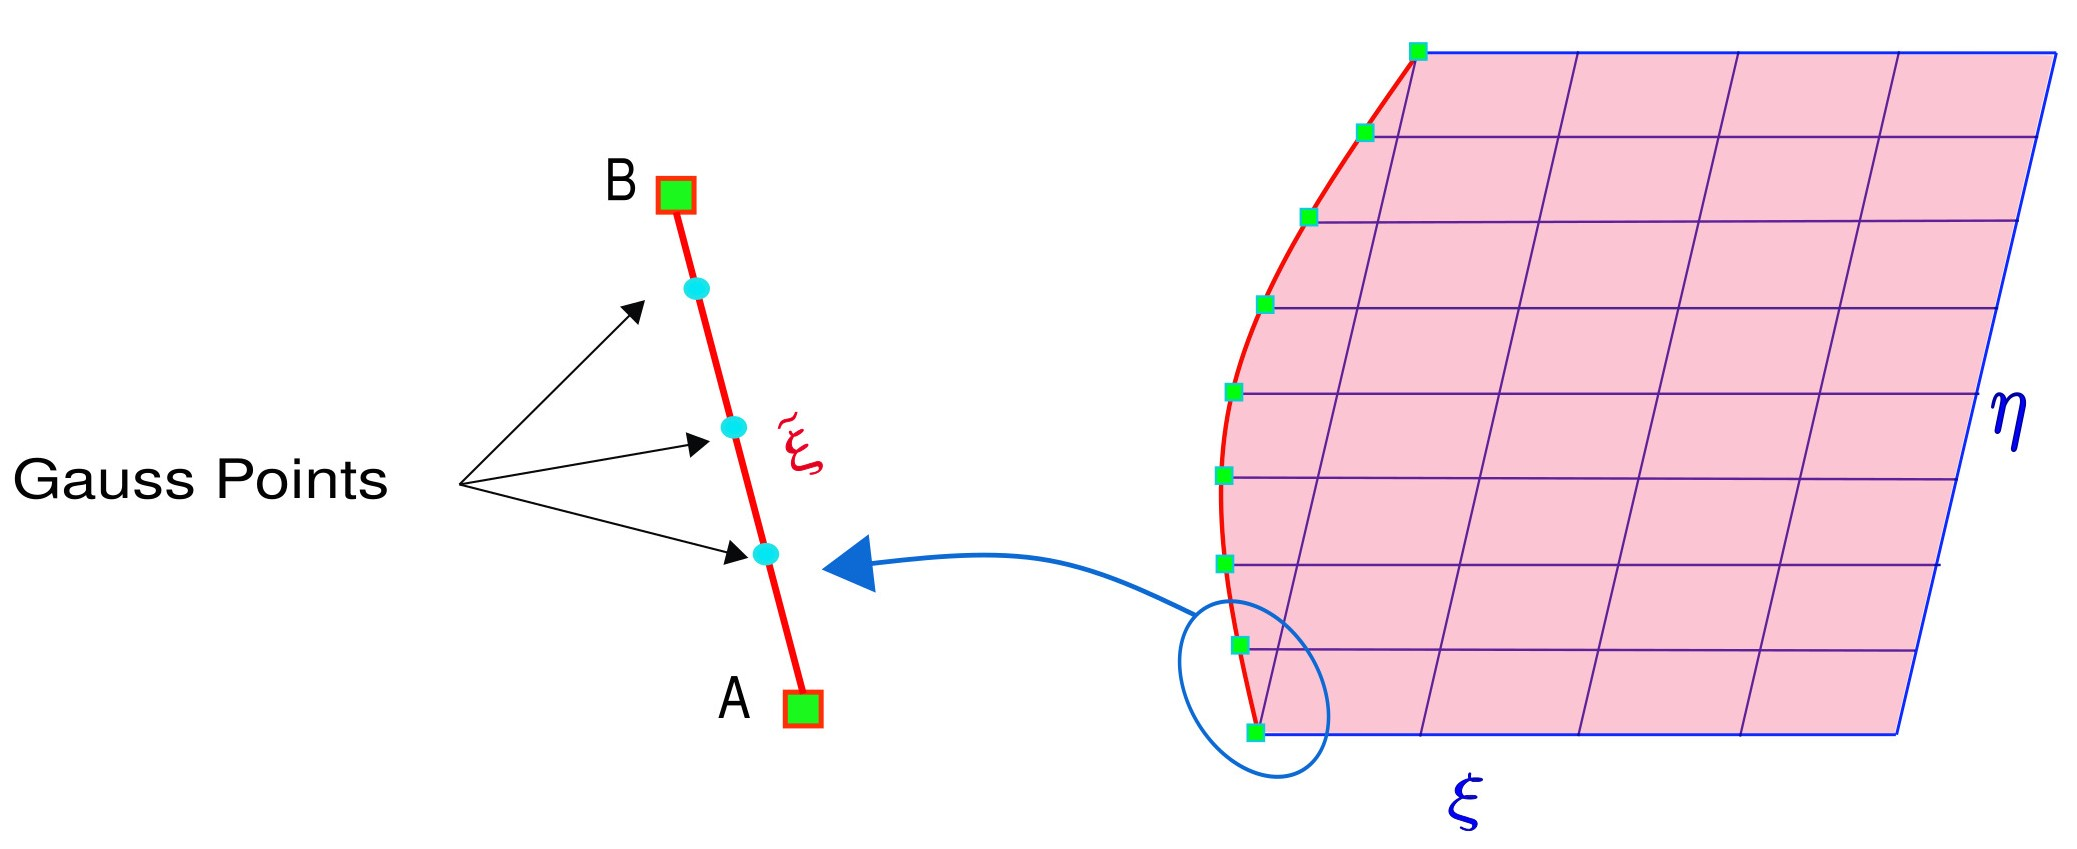
\includegraphics[width=0.8\textwidth]{Images/weak-dirichlet_demo.jpg}
\caption{Weak Dirichlet along the boundary curve $\Gamma_c$}
\label{fig:weak_dir_demo}
\end{figure}}

\subsection{Element creation and integration procedure for Weak Dirichlet boundary condition}
A step by step procedure is explained below to obtain the integration elements on the boundary curve (see figure \ref{fig:weak_dir_demo} ):
\begin{enumerate}
    \item Intersection of the boundary curve with the isoparametric curves (knot lines) of the patch is found. See the green ($\tilde{\xi_{i}}$) rectangular points in the parametric space of edge curve of the patches.
    \item Each section of the edge curve of patch 1 within the intersection points form the edge elements.
    \item Gauss points are found on each such element (see blue points) like AB with representation on the edge curve ($\tilde{\xi_{g_i}}$) as well as on the patch $(\xi_{g_i},\eta_{g_i})$.

\end{enumerate}

\begin{table}[htbp]
    \centering
    \renewcommand{\arraystretch}{1.2}
    \begin{tabular}{|c|c|c|c|c|}
        \hline
      \multirow{2}{*}{\textbf{Edge ($\tilde{\xi_{g1_i}}$)}} & \multirow{2}{*}{\textbf{Gauss Wt}} & \multirow{2}{*}{$\mathbf{J_3}$} & \multicolumn{2}{c|}{\textbf{Patch }}  \\ \cline{4-5}
      &  \textbf{$\xi_{g1_i}$} & \textbf{$\eta_{g1_i}$} & \textbf{$\xi_{g2_i}$} & \textbf{$\eta_{g2_i}$} \\ \hline
         0.37 & 8/9 & 0.7 & 15 & 4   \\ 
        .. & .. & .. & .. & ..  \\ 
        .. & .. & .. & .. & .. \\ \hline
    \end{tabular}
    \caption{Data Structure for Weak Dirichlet boundary curve}
\end{table}
\subsection{Element creation and integration procedure for coupling patches}

A step by step procedure is explained below to obtain the integration elements on the coupling curve (see figure \ref{fig:patch_couple_1} ):

\begin{enumerate}
    \item Intersection of the coupling curve with the isoparametric curves (knot lines) of both the patches are found. See the red ($\tilde{\xi_{1_i}}$) and green ($\tilde{\xi_{2_i}}$) rectangular points in the parametric space of edge curves of the patches 1 and 2 respectively.
    \item Since the integration is to be performed on the primary patch (here 1), the green points are to be projected on to the edge curve of patch 1. The follwing method is adopted:
    \begin{enumerate}
        \item The patch coordinates (here patch 2) $(\xi_{2_i},\eta_{2_i})$ of each green point ($\tilde{\xi_{2_i}}$) of its edge curve are found.
        \item Then physical point coordinates $(x_{2_i},y_{2_i},z_{2_i})$ corresponding to $(\xi_{2_i},\eta_{2_i})$ are found.
        \item Each physical point $(x_{2_i},y_{2_i},z_{2_i})$ is projected on the primary patch 1 and the patch coordinates $(\xi_{1_i},\eta_{1_i})$ are found.
        \item Finally these points are projected on to the edge curve of the first patch (see green points on patch 1)
    \end{enumerate}
    \item Each section of the edge curve of patch 1 within the intersection and projected points (red and green respectively) form the edge elements.
    \item Gauss points are found on each such element (see blue points) like AB with representation on the edge curve ($\tilde{\xi_{g1_i}}$) as well as on the patch $(\xi_{g1_i},\eta_{g1_i})$.
    \item These Gauss points are projected on the patch 2 as well using the methods explained in steps 2(b) and 2(c) to get the points $(\xi_{g2_i},\eta_{g2_i})$
\end{enumerate}
\textbf{\begin{figure}[H]
\centering
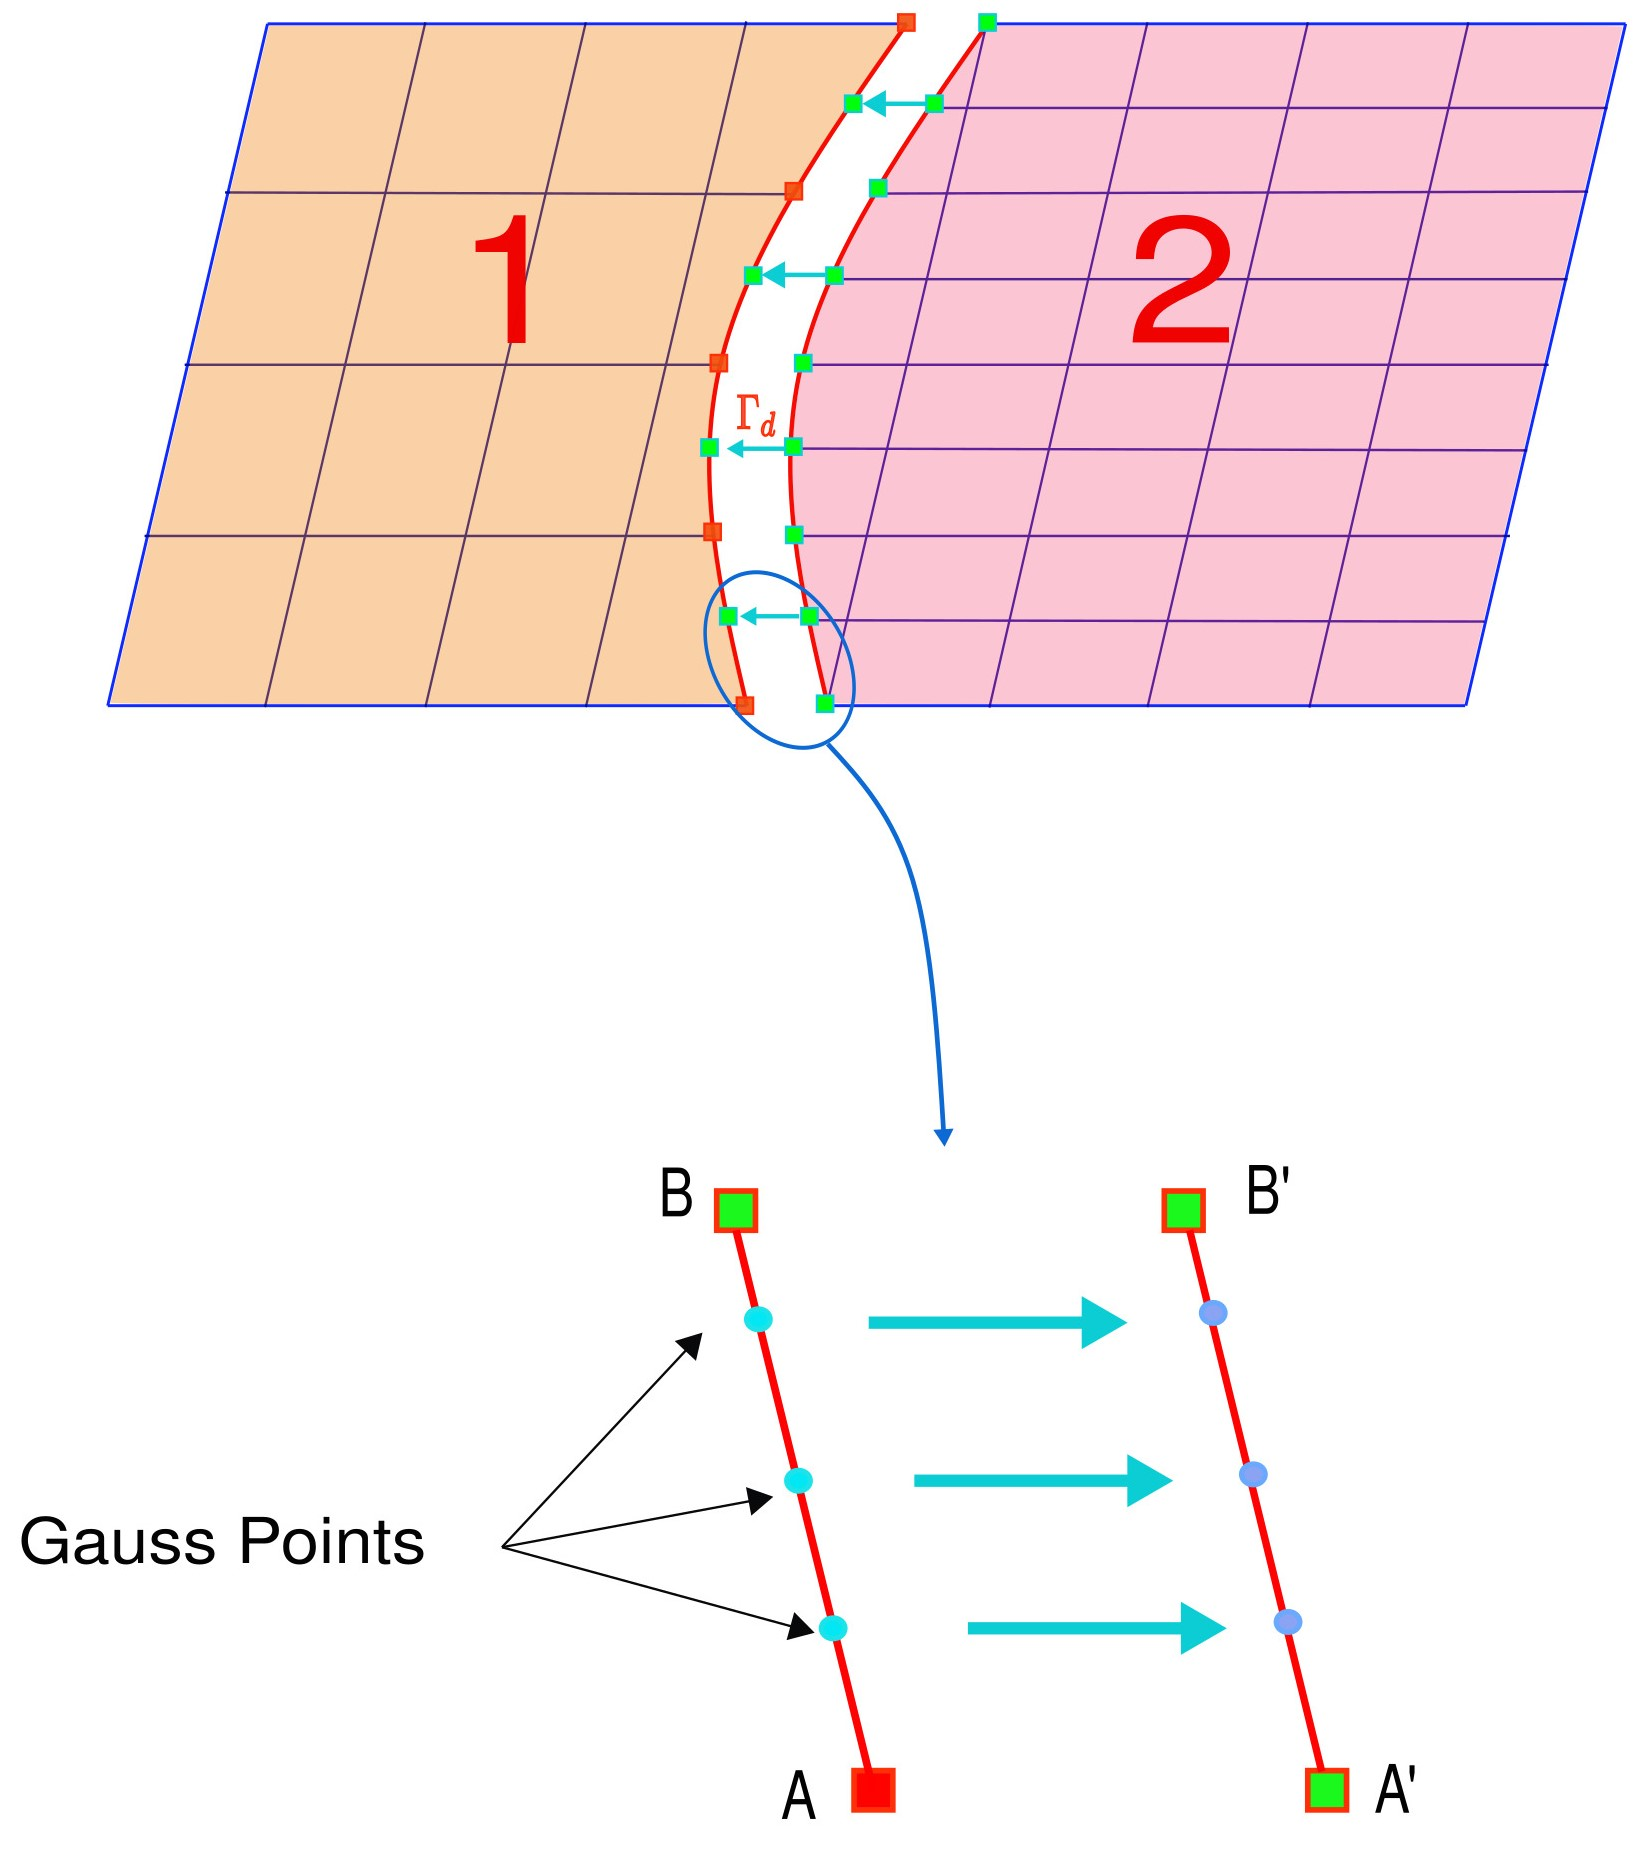
\includegraphics[width=0.8\textwidth]{Images/patch_coupling_1.jpg}
\caption{Two plane patches to be coupled along $\Gamma_c$}
\label{fig:patch_couple_1}
\end{figure}}

\begin{table}[htbp]
    \centering
    \renewcommand{\arraystretch}{1.2}
    \begin{tabular}{|c|c|c|c|c|c|c|}
        \hline
      \multirow{2}{*}{\textbf{Edge ($\tilde{\xi_{g1_i}}$)}} & \multirow{2}{*}{\textbf{Gauss Wt}} & \multirow{2}{*}{$\mathbf{J_3}$} & \multicolumn{2}{c|}{\textbf{Patch 1}} & \multicolumn{2}{c|}{\textbf{Patch 2}} \\ \cline{4-7}
      & & & \textbf{$\xi_{g1_i}$} & \textbf{$\eta_{g1_i}$} & \textbf{$\xi_{g2_i}$} & \textbf{$\eta_{g2_i}$} \\ \hline
         0.37 & 8/9 & 0.7 & 15 & 4 & 0 & 3  \\ 
        .. & .. & .. & .. & .. & .. & .. \\ 
        .. & .. & .. & .. & .. & .. & .. \\ \hline
    \end{tabular}
    \caption{Data Structure for coupling curve}
\end{table}


\chapter{Results} \label{chap: Results}
\section{Isogeometric Analysis of Timoshenko Beam}
The deformation results from the Isogeometric Analysis of Timoshenko cantilever Beam is converged to the analytical solution (Figure 5).
\begin{figure}[htbp]
\centering
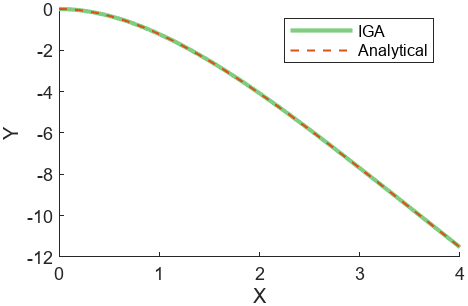
\includegraphics[width=0.6\textwidth]{Images/beam_deform.png}
\caption{Timoshenko Beam Deformation from Isogeometric Analysis and Analytical Solution}
\label{fig:timobeam}
\end{figure}


\begin{figure}[H]
\centering
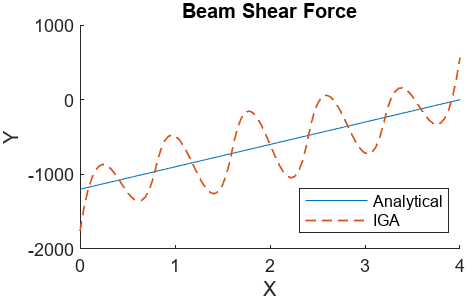
\includegraphics[width=0.6\textwidth]{Images/beam shear force.png}
\caption{Shear Force distribution of Timoshenko beam from Isogeometric Analysis and Analytical Solution}
\label{fig:RMplateV}
\end{figure}
Figure 6 illustrates there is the oscillation around the analytical solution for Shear Force distribution of Timoshenko cantilever beam using Isogeometric Analysis. This is caused by shear locking due to numerical integration.

\section{Isogeometric Analysis of Reissner-Mindlin plate}
The deformation results from the Isogeometric Analysis of Reissner-Mindlin cantilever plate is converged to the analytical solution (Figure 7).
\begin{figure}[htbp]
\centering
\includegraphics[width=0.8\textwidth]{Images/plate_deform.jpg}
\caption{Deformation of Reissner-Mindlin plate from Isogeometric Analysis and Analytical Solution}
\label{fig:RMplate}
\end{figure}


\begin{figure}[H]
\centering
\includegraphics[width=0.7\textwidth]{Images/plate_shear.jpg}
\caption{Shear Force distribution of Reissner-Mindlin plate from Isogeometric Analysis and Analytical Solution}
\label{fig:RM}
\end{figure}

Figure 8 illustrates there is the oscillation around the analytical solution for Shear Force distribution of Reissner-Mindlin cantilever plate using Isogeometric Analysis which is caused by shear locking.
\section{Isogeometric Analysis of a Trimmed surface}

\begin{figure}[htbp]
\centering
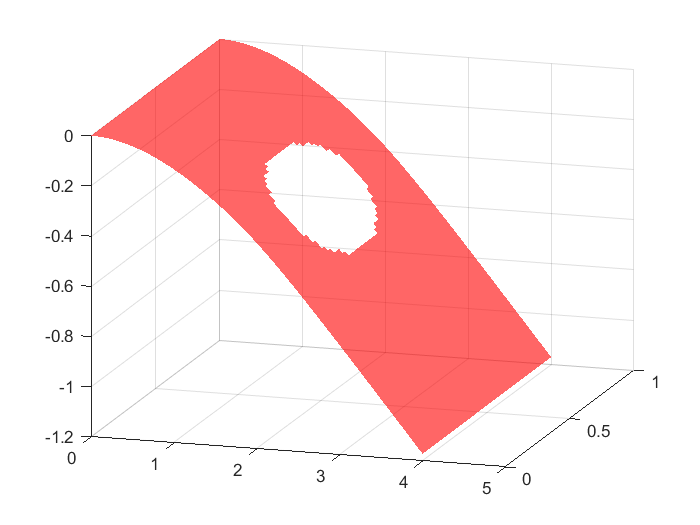
\includegraphics[width=0.7\textwidth]{Images/trim_plate_deform.png}
\caption{Deformation of a rectangle surface trimmed by a circle using Isogeometric Analysis}
\label{fig:Tridef}
\end{figure}

\begin{figure}[H]
\centering
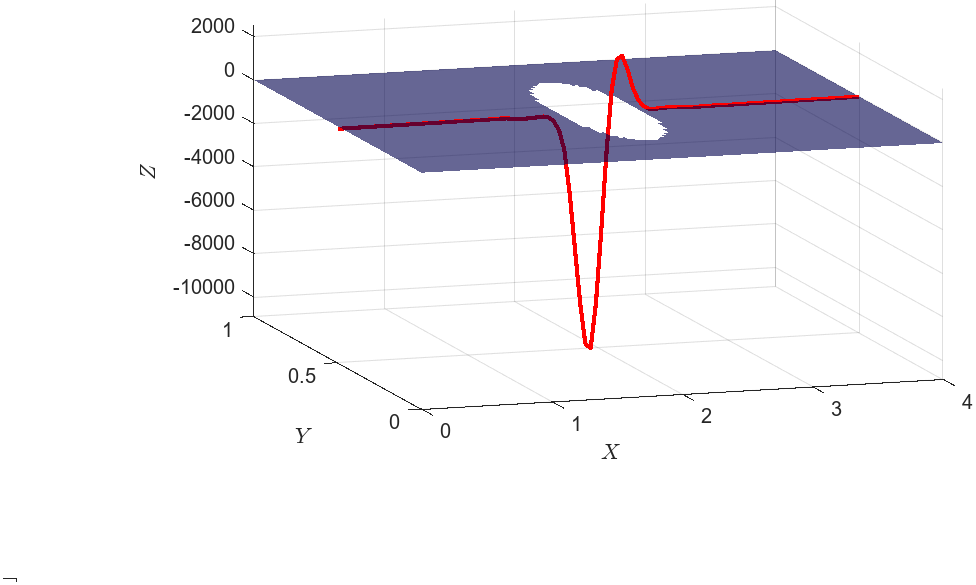
\includegraphics[width=0.8\textwidth]{Images/trim_shear.png}
\caption{Shear force distribution of a rectangle surface trimmed by a circle using Isogeometric Analysis}
\label{fig:TriShear}
\end{figure}
\clearpage

\appendix

\chapter*{Appendix} \label{chap: Appendix}
\section*{A  Python Scripts}
\label{app:A}
The code for getting NURBS information is shown here. Both of the Python scripts are extended versions of  \href{https://github.com/tpaviot/pythonocc-demos}{Demo examples from git repository of PythonOCC}. The flowchart of how the extraction of NURBS information works through PythonOCC is shown in Figure \ref{fig:pythonoccFlowchart}.
\begin{figure}[H]
\centering
\includegraphics[width=0.8\textwidth]{Images/flowcaht.png}
\caption{Flowchart of Extracting NURBS information through PythonOCC}
\label{fig:pythonoccFlowchart}
\end{figure}

\subsection*{A1  curveNURBS}\label{Appendix_A1_curveNURBS}
% Define custom colors
\definecolor{vscode-purple}{rgb}{0.502, 0, 0.502}
\definecolor{vscode-green}{rgb}{0, 0.502, 0}
\definecolor{vscode-blue}{rgb}{0, 0, 0.502}
\definecolor{vscode-yellow}{rgb}{0.502, 0.502, 0}
\definecolor{backcolour}{rgb}{0.95,0.95,0.92}% Light gray background

% Define custom Python style
\lstdefinestyle{python}{
    language=Python,
    backgroundcolor=\color{backcolour},
    commentstyle=\color{vscode-green},
    keywordstyle=\color{vscode-blue},
    numberstyle=\tiny\color{vscode-yellow},
    stringstyle=\color{vscode-purple},
    basicstyle=\ttfamily\small,
    breakatwhitespace=false,
    breaklines=true,
    captionpos=b,
    keepspaces=true,
    showspaces=false,
    showstringspaces=false,
    showtabs=false,
    tabsize=4,
    extendedchars=true,
    inputencoding=utf8,
    frame=tb,
    framerule=1pt,
    numbersep=5pt,
    numbers=left,
    stepnumber=1,  % Display every line number
    firstnumber=1   % Specify the starting line number
}

\lstset{style=python}
\begin{adjustwidth}{-0.5cm}{-0.5cm}
\begin{lstlisting}{language=Python}
from OCC.Core.BRepBuilderAPI import BRepBuilderAPI_NurbsConvert
from OCC.Core.BRepAdaptor import BRepAdaptor_Curve
from OCC.Extend.DataExchange import read_iges_file
from OCC.Extend.TopologyUtils import TopologyExplorer
from OCC.Core.GeomAbs import GeomAbs_BSplineCurve
import numpy as np

def getNURBS_Curve(iges_file_path):
    
    #read iges file
    base_shape = read_iges_file(iges_file_path)
    
    # conversion to a nurbs representation
    nurbs_converter = BRepBuilderAPI_NurbsConvert(base_shape, True)
    
    # nurbs_converter.Perform()
    converted_shape = nurbs_converter.Shape()
    expl = TopologyExplorer(converted_shape)
    
    # loop over edges
    cur_idx = 1

    for edge in expl.edges():
        print("=== Edge %i ===" % cur_idx)
        curv = BRepAdaptor_Curve(edge)
        
        # check each of the edge if it is a BSpline curve
        curv_type = curv.GetType()
        if not curv_type == GeomAbs_BSplineCurve:
            raise AssertionError("the face was not converted to a 
            GeomAbs_BSplineCurve")
        
        # Polynomial Order
        bcurve = curv.BSpline()
        curveDegree = bcurve.Degree()
        print("Degree:", curveDegree)
    
        #knots array
        knots = bcurve.Knots()
        print("\nknots:")
        knotArr=[]
        for i in range(bcurve.NbKnots()):
            knotArr.append(knots.Value(i + 1))
        knotArray = [knotArr[0]] * (curveDegree+1) + knotArr[1:-1] 
        + [knotArr[-1]] * (curveDegree+1)
        print(','.join(map(str, knotArray)))
        
        # weights
        weights = bcurve.Weights()
        # PythonOCC does not return weights if all weights are equal to one.
        if weights is not None:
            weightArray = np.zeros((1,bcurve.NbPoles()))
            for i in range(bcurve.NbPoles()):
                weightArray[0,i] = weights.Value(i + 1)     
        else:
            # If weights are not returned, we set all equal to one
            weightArray=np.ones((1,bcurve.NbPoles()))
        print("\nweight: ")
        print(weightArray)
            
        # control points (aka poles)
        poles = bcurve.Poles()
 
        if poles is not None:
            poleArray = []
            print("\nPoles (control points):")
            for i in range(bcurve.NbPoles()):
                    p = poles.Value(i + 1)
                    poleArray.append(p.X())
                    poleArray.append(p.Y())
                    poleArray.append(p.Z())
        print(poleArray)
        
        print()
        cur_idx += 1
\end{lstlisting}
\end{adjustwidth}

\subsection*{A2  surfaceNURBS}\label{Appendix_A2_surfaceNURBS}
% Define custom colors
\definecolor{vscode-purple}{rgb}{0.502, 0, 0.502}
\definecolor{vscode-green}{rgb}{0, 0.502, 0}
\definecolor{vscode-blue}{rgb}{0, 0, 0.502}
\definecolor{vscode-yellow}{rgb}{0.502, 0.502, 0}
\definecolor{backcolour}{rgb}{0.95,0.95,0.92}% Light gray background

% Define custom Python style
\lstdefinestyle{python2}{
    language=Python,
    backgroundcolor=\color{backcolour},
    commentstyle=\color{vscode-green},
    keywordstyle=\color{vscode-blue},
    numberstyle=\tiny\color{vscode-yellow},
    stringstyle=\color{vscode-purple},
    basicstyle=\ttfamily\small,
    breakatwhitespace=false,
    breaklines=true,
    captionpos=b,
    keepspaces=true,
    showspaces=false,
    showstringspaces=false,
    showtabs=false,
    tabsize=4,
    extendedchars=true,
    inputencoding=utf8,
    frame=tb,
    framerule=1pt,
    numbers=left,
    numbersep=5pt,
}

% Apply the style
\lstset{style=python2}
\begin{adjustwidth}{-0.5cm}{-0.5cm}

\begin{lstlisting}{language=Python}
import numpy as np
from OCC.Core.BRepBuilderAPI import BRepBuilderAPI_NurbsConvert
from OCC.Core.BRepAdaptor import BRepAdaptor_Surface
from OCC.Extend.DataExchange import read_iges_file
from OCC.Extend.TopologyUtils import TopologyExplorer
from OCC.Core.GeomAbs import GeomAbs_BSplineSurface

def getNURBS_Surface(iges_file_path):
    
    #read iges file
    base_shape = read_iges_file(iges_file_path)
    
    # conversion to a nurbs representation
    nurbs_converter = BRepBuilderAPI_NurbsConvert(base_shape, True)
    converted_shape = nurbs_converter.Shape()
    
    expl = TopologyExplorer(converted_shape)
    
    # loop over faces
    fc_idx = 1
    for face in expl.faces():
        print("=== Face %i ===" % fc_idx)
        surf = BRepAdaptor_Surface(face, True)
        
        # check each of the face is a BSpline surface
        surf_type = surf.GetType()
        if not surf_type == GeomAbs_BSplineSurface:
            raise AssertionError("the face was not converted to a 
            GeomAbs_BSplineSurface")
        
        # Polynomial Order
        bsrf = surf.BSpline()
        UCurveDegree = bsrf.UDegree()
        VCurveDegree = bsrf.VDegree()
        print("UDegree:", UCurveDegree )
        print("VDegree:", VCurveDegree )
        
        # uknots array
        uknots = bsrf.UKnots()
        print("\nUknots:")
        UknotArr=[]
        for i in range(bsrf.NbUKnots()):
            UknotArr.append(uknots.Value(i+1))
        UknotArr = [UknotArr[0]] * (UCurveDegree+1) + UknotArr[1:-1] 
        + [UknotArr[-1]] * (UCurveDegree+1)
        print(','.join(map(str, UknotArr)))
        
        # vknots array
        vknots = bsrf.VKnots()
        print("Vknots:")
        VknotArr=[]
        for i in range(bsrf.NbVKnots()):
            VknotArr.append(vknots.Value(i+1))
        VknotArr = [VknotArr[0]] * (VCurveDegree+1) + VknotArr[1:-1] 
        + [VknotArr[-1]] * (VCurveDegree+1)
        print(','.join(map(str, VknotArr)))

        # Weights 
        weights = bsrf.Weights()
        if weights is not None:
            weightMatrix=np.zeros((bsrf.NbUPoles(),bsrf.NbVPoles()))
            for i in range(bsrf.NbUPoles()):
                for j in range(bsrf.NbVPoles()):
                    weightMatrix[i,j] = weights.Value(i + 1, j + 1)       
        # weights can be None
        else:
            weightMatrix=np.ones((bsrf.NbUPoles(),bsrf.NbVPoles()))    
        print("\nweight: \n", weightMatrix)

        # control Points
        poles = bsrf.Poles()
        if poles is not None:
            polesArr = []
            print("\nPoles (control points):")
            for i in range(bsrf.NbUPoles()):
                for j in range(bsrf.NbVPoles()):
                    p = poles.Value(i + 1, j + 1)
                    polesArr.append(p.X())
                    polesArr.append(p.Y())
                    polesArr.append(p.Z())
        print(polesArr)

        print()
        fc_idx += 1
\end{lstlisting}
\end{adjustwidth}
\subsection*{A3  trimmedPlate}\appendix\label{app Appendix_A3_trimPlate}
% Define custom colors
\definecolor{vscode-purple}{rgb}{0.502, 0, 0.502}
\definecolor{vscode-green}{rgb}{0, 0.502, 0}
\definecolor{vscode-blue}{rgb}{0, 0, 0.502}
\definecolor{vscode-yellow}{rgb}{0.502, 0.502, 0}
\definecolor{backcolour}{rgb}{0.95,0.95,0.92}% Light gray background

% Define custom Python style
\lstdefinestyle{python2}{
    language=Python,
    backgroundcolor=\color{backcolour},
    commentstyle=\color{vscode-green},
    keywordstyle=\color{vscode-blue},
    numberstyle=\tiny\color{vscode-yellow},
    stringstyle=\color{vscode-purple},
    basicstyle=\ttfamily\small,
    breakatwhitespace=false,
    breaklines=true,
    captionpos=b,
    keepspaces=true,
    showspaces=false,
    showstringspaces=false,
    showtabs=false,
    tabsize=4,
    extendedchars=true,
    inputencoding=utf8,
    frame=tb,
    framerule=1pt,
    numbers=left,
    numbersep=5pt,
}

% Apply the style
\lstset{style=python2}
\begin{adjustwidth}{-0.5cm}{-0.5cm}

\begin{lstlisting}{language=Python}
from OCC.Core.BRep import BRep_Tool
from OCC.Core.BRepAdaptor import BRepAdaptor_CompCurve
from OCC.Core.Geom import Geom_BSplineCurve,Geom_BSplineSurface
from OCC.Core.BRepBuilderAPI import BRepBuilderAPI_MakeEdge, BRepBuilderAPI_MakeWire
from OCC.Core.Geom2dConvert import geom2dconvert  
from OCC.Core.TColgp import TColgp_Array1OfPnt2d
from OCC.Core.TColStd import TColStd_Array1OfInteger, TColStd_Array1OfReal
from OCC.Core.TopExp import TopExp_Explorer  
from OCC.Core.TopAbs import TopAbs_EDGE,TopAbs_WIRE,TopAbs_FACE
from OCC.Core.TopoDS import topods
from OCC.Core.ShapeAnalysis import shapeanalysis
from OCC.Extend.DataExchange import read_iges_file
from OCC.Display.SimpleGui import init_display
import numpy as np
def getWireData(_OCC_outerWire, _OCC_wire):
  """
  Receives a TopoDS_SHAPE class with a Wire type and converts its data to python type
  \param[in] _OCC_wire	class: TopoDS_SHAPE	type: Wire
  \return inner
  \return noTrCurves
  """
  # Determine inner or outer boundary loop
  if _OCC_wire.IsEqual(_OCC_outerWire):
    inner = False
  else:
    inner = True

  # Count number of trimming curves in the loop
  noTrCurves = 0  
  edgeExplorer = TopExp_Explorer(_OCC_wire, TopAbs_EDGE)
  while edgeExplorer.More():
    noTrCurves += 1
    edgeExplorer.Next()
  
  return inner, noTrCurves


def getOuterWire(_OCC_face):
  """
  \param[in] _OCC_face	class: TopoDS_SHAPE	type: Face
  \return OCC_outerWire
  """
  
  OCC_outerWire = shapeanalysis.OuterWire(topods.Face(_OCC_face))

  return OCC_outerWire

def getEdgeDataWithOrientation(_OCC_edge, _OCC_wire, _OCC_face):
  """
  \param[in] _OCC_edge	class: TopoDS_SHAPE	type: Edge
  \param[in] _OCC_wire	class: TopoDS_SHAPE	type: Wire
  \param[in] _OCC_face	class: TopoDS_SHAPE	type: Face
  \return direction
  \return pDegree
  \return uKnotVector
  \return uNoCPs
  \return CPNet
  """
  # Convert a topological TopoDS_EDGE into Geom2d_BSplineCurve
  OCC_handle_curve2d, activeRangeBegin, activeRangeEnd = BRep_Tool.CurveOnSurface(topods.Edge(_OCC_edge), topods.Face(_OCC_face))
  OCC_bsplineCurve2d = geom2dconvert.CurveToBSplineCurve(OCC_handle_curve2d)#.GetObject()
  
  if OCC_bsplineCurve2d.IsPeriodic(): 
    print("Found periodic curve!")
    OCC_bsplineCurve2d.SetNotPeriodic()
  # Curve direction 
  direction = (_OCC_wire.Orientation() + _OCC_edge.Orientation() + 1)%2
  # pDegree
  pDegree = OCC_bsplineCurve2d.Degree()
  # No of Knots
  OCC_uNoKnots = OCC_bsplineCurve2d.NbKnots()
  # Knot vector
  OCC_uKnotMulti = TColStd_Array1OfInteger(1,OCC_uNoKnots)
  OCC_bsplineCurve2d.Multiplicities(OCC_uKnotMulti)
  uNoKnots = 0
  for ctr in range(1,OCC_uNoKnots+1): uNoKnots += OCC_uKnotMulti.Value(ctr)
  OCC_uKnotSequence = TColStd_Array1OfReal(1,uNoKnots)
  OCC_bsplineCurve2d.KnotSequence(OCC_uKnotSequence)
  uKnotVector = []
  for iKnot in range(1,uNoKnots+1): uKnotVector.append(OCC_uKnotSequence.Value(iKnot))
  # No of CPs
  uNoCPs = OCC_bsplineCurve2d.NbPoles()
  # CPs
  OCC_CPnet = TColgp_Array1OfPnt2d(1,uNoCPs)
  OCC_bsplineCurve2d.Poles(OCC_CPnet)
  # CP weights
  OCC_CPweightNet = TColStd_Array1OfReal(1,uNoCPs)
  OCC_bsplineCurve2d.Weights(OCC_CPweightNet)
  CPNet = []
  for iCP in range(1,uNoCPs+1):
    OCC_CP = OCC_CPnet.Value(iCP)
    OCC_CPweight = OCC_CPweightNet.Value(iCP)
    CPNet.extend([OCC_CP.X(), OCC_CP.Y(), 0.0, OCC_CPweight])
    
  # Create a linear space with 25 points
  start_value = uKnotVector[0]
  end_value = uKnotVector[-1] 
  num_points = 25
  linear_space = np.linspace(start_value, end_value, num_points)
  num_points = 25
  points_on_curve = [OCC_bsplineCurve2d.Value(i) for i in linear_space ]
  x_coordinates=[]
  y_coordinates=[]
  for point in points_on_curve:
    x_coordinates.append(point.X())
    y_coordinates.append(point.Y()) 
  return x_coordinates,y_coordinates

## MAIN CODE STARTS HERE
iges_file_path = "C:\\Users\\oslon\\Desktop\\MSc\\Thesis\\Code Scripts\\trimmedRect.igs" 
_OCC_nurbsShape = read_iges_file(iges_file_path)
print(_OCC_nurbsShape.ShapeType())

# Face explorer to gather the geometrical information

faceExplorer = TopExp_Explorer(_OCC_nurbsShape, TopAbs_FACE)
while faceExplorer.More():
  currentFace = faceExplorer.Current()
  faceExplorer.Next()

  ## Gather patch trimming loop info
  # Get outer wire
  OCC_outerWire = getOuterWire(currentFace)
  
  
  faceWireExplorer = TopExp_Explorer(currentFace, TopAbs_WIRE) # This will explore outer and inner wires
  
  while faceWireExplorer.More():        # Loop through all wires (outer and inner)
    
    currentFaceWire = faceWireExplorer.Current()
    faceWireExplorer.Next()

    # Collect wire data
    inner, noTrCurves = getWireData(OCC_outerWire, currentFaceWire)   # check if the wire is exterior or interior
    #note: get wire data takes a wire and checks if it is exterior or interior. noTrCurves returns number...  
    # of edges in that wire (external or internal) 
 
    faceWireEdgeExplorer = TopExp_Explorer(currentFaceWire, TopAbs_EDGE)
    
    par_range=[]
    X_trim_vec=[]
    Y_trim_vec=[]
    if inner:           # For only interior trimming wire which is one in my case of circular trimming curve
      
      while faceWireEdgeExplorer.More():        # Checking the edges in the wire, 4 in my case
        currentFaceWireEdge = faceWireEdgeExplorer.Current()
        faceWireEdgeExplorer.Next()
        x,y = getEdgeDataWithOrientation(currentFaceWireEdge, currentFaceWire, currentFace)
        X_trim_vec.extend(x)
        Y_trim_vec.extend(y)
        
        
    #print(X_trim_vec)
        
      
 
    
  





\end{lstlisting}
\end{adjustwidth}
\newpage
\bibliographystyle{plain}
\bibliography{citations}

\end{document}
